% Options for packages loaded elsewhere
\PassOptionsToPackage{unicode}{hyperref}
\PassOptionsToPackage{hyphens}{url}
%
\documentclass[
]{book}
\usepackage{amsmath,amssymb}
\usepackage{setspace}
\usepackage{iftex}
\ifPDFTeX
  \usepackage[T1]{fontenc}
  \usepackage[utf8]{inputenc}
  \usepackage{textcomp} % provide euro and other symbols
\else % if luatex or xetex
  \usepackage{unicode-math} % this also loads fontspec
  \defaultfontfeatures{Scale=MatchLowercase}
  \defaultfontfeatures[\rmfamily]{Ligatures=TeX,Scale=1}
\fi
\usepackage{lmodern}
\ifPDFTeX\else
  % xetex/luatex font selection
\fi
% Use upquote if available, for straight quotes in verbatim environments
\IfFileExists{upquote.sty}{\usepackage{upquote}}{}
\IfFileExists{microtype.sty}{% use microtype if available
  \usepackage[]{microtype}
  \UseMicrotypeSet[protrusion]{basicmath} % disable protrusion for tt fonts
}{}
\makeatletter
\@ifundefined{KOMAClassName}{% if non-KOMA class
  \IfFileExists{parskip.sty}{%
    \usepackage{parskip}
  }{% else
    \setlength{\parindent}{0pt}
    \setlength{\parskip}{6pt plus 2pt minus 1pt}}
}{% if KOMA class
  \KOMAoptions{parskip=half}}
\makeatother
\usepackage{xcolor}
\usepackage[footnotesep=20pt]{geometry}
\usepackage{color}
\usepackage{fancyvrb}
\newcommand{\VerbBar}{|}
\newcommand{\VERB}{\Verb[commandchars=\\\{\}]}
\DefineVerbatimEnvironment{Highlighting}{Verbatim}{commandchars=\\\{\}}
% Add ',fontsize=\small' for more characters per line
\usepackage{framed}
\definecolor{shadecolor}{RGB}{248,248,248}
\newenvironment{Shaded}{\begin{snugshade}}{\end{snugshade}}
\newcommand{\AlertTok}[1]{\textcolor[rgb]{0.94,0.16,0.16}{#1}}
\newcommand{\AnnotationTok}[1]{\textcolor[rgb]{0.56,0.35,0.01}{\textbf{\textit{#1}}}}
\newcommand{\AttributeTok}[1]{\textcolor[rgb]{0.13,0.29,0.53}{#1}}
\newcommand{\BaseNTok}[1]{\textcolor[rgb]{0.00,0.00,0.81}{#1}}
\newcommand{\BuiltInTok}[1]{#1}
\newcommand{\CharTok}[1]{\textcolor[rgb]{0.31,0.60,0.02}{#1}}
\newcommand{\CommentTok}[1]{\textcolor[rgb]{0.56,0.35,0.01}{\textit{#1}}}
\newcommand{\CommentVarTok}[1]{\textcolor[rgb]{0.56,0.35,0.01}{\textbf{\textit{#1}}}}
\newcommand{\ConstantTok}[1]{\textcolor[rgb]{0.56,0.35,0.01}{#1}}
\newcommand{\ControlFlowTok}[1]{\textcolor[rgb]{0.13,0.29,0.53}{\textbf{#1}}}
\newcommand{\DataTypeTok}[1]{\textcolor[rgb]{0.13,0.29,0.53}{#1}}
\newcommand{\DecValTok}[1]{\textcolor[rgb]{0.00,0.00,0.81}{#1}}
\newcommand{\DocumentationTok}[1]{\textcolor[rgb]{0.56,0.35,0.01}{\textbf{\textit{#1}}}}
\newcommand{\ErrorTok}[1]{\textcolor[rgb]{0.64,0.00,0.00}{\textbf{#1}}}
\newcommand{\ExtensionTok}[1]{#1}
\newcommand{\FloatTok}[1]{\textcolor[rgb]{0.00,0.00,0.81}{#1}}
\newcommand{\FunctionTok}[1]{\textcolor[rgb]{0.13,0.29,0.53}{\textbf{#1}}}
\newcommand{\ImportTok}[1]{#1}
\newcommand{\InformationTok}[1]{\textcolor[rgb]{0.56,0.35,0.01}{\textbf{\textit{#1}}}}
\newcommand{\KeywordTok}[1]{\textcolor[rgb]{0.13,0.29,0.53}{\textbf{#1}}}
\newcommand{\NormalTok}[1]{#1}
\newcommand{\OperatorTok}[1]{\textcolor[rgb]{0.81,0.36,0.00}{\textbf{#1}}}
\newcommand{\OtherTok}[1]{\textcolor[rgb]{0.56,0.35,0.01}{#1}}
\newcommand{\PreprocessorTok}[1]{\textcolor[rgb]{0.56,0.35,0.01}{\textit{#1}}}
\newcommand{\RegionMarkerTok}[1]{#1}
\newcommand{\SpecialCharTok}[1]{\textcolor[rgb]{0.81,0.36,0.00}{\textbf{#1}}}
\newcommand{\SpecialStringTok}[1]{\textcolor[rgb]{0.31,0.60,0.02}{#1}}
\newcommand{\StringTok}[1]{\textcolor[rgb]{0.31,0.60,0.02}{#1}}
\newcommand{\VariableTok}[1]{\textcolor[rgb]{0.00,0.00,0.00}{#1}}
\newcommand{\VerbatimStringTok}[1]{\textcolor[rgb]{0.31,0.60,0.02}{#1}}
\newcommand{\WarningTok}[1]{\textcolor[rgb]{0.56,0.35,0.01}{\textbf{\textit{#1}}}}
\usepackage{longtable,booktabs,array}
\usepackage{calc} % for calculating minipage widths
% Correct order of tables after \paragraph or \subparagraph
\usepackage{etoolbox}
\makeatletter
\patchcmd\longtable{\par}{\if@noskipsec\mbox{}\fi\par}{}{}
\makeatother
% Allow footnotes in longtable head/foot
\IfFileExists{footnotehyper.sty}{\usepackage{footnotehyper}}{\usepackage{footnote}}
\makesavenoteenv{longtable}
\usepackage{graphicx}
\makeatletter
\def\maxwidth{\ifdim\Gin@nat@width>\linewidth\linewidth\else\Gin@nat@width\fi}
\def\maxheight{\ifdim\Gin@nat@height>\textheight\textheight\else\Gin@nat@height\fi}
\makeatother
% Scale images if necessary, so that they will not overflow the page
% margins by default, and it is still possible to overwrite the defaults
% using explicit options in \includegraphics[width, height, ...]{}
\setkeys{Gin}{width=\maxwidth,height=\maxheight,keepaspectratio}
% Set default figure placement to htbp
\makeatletter
\def\fps@figure{htbp}
\makeatother
\ifLuaTeX
  \usepackage{luacolor}
  \usepackage[soul]{lua-ul}
\else
  \usepackage{soul}
\fi
\setlength{\emergencystretch}{3em} % prevent overfull lines
\providecommand{\tightlist}{%
  \setlength{\itemsep}{0pt}\setlength{\parskip}{0pt}}
\setcounter{secnumdepth}{5}
\ifLuaTeX
  \usepackage{selnolig}  % disable illegal ligatures
\fi
\usepackage[]{natbib}
\bibliographystyle{plainnat}
\nocite{R-base, R-bookdown, R-rmarkdown, R-dplyr, R-webexercises, R-ggplot2}
\usepackage{bookmark}
\IfFileExists{xurl.sty}{\usepackage{xurl}}{} % add URL line breaks if available
\urlstyle{same}
\hypersetup{
  pdftitle={Psychological Research in R},
  pdfauthor={Anni Tave Overlander},
  hidelinks,
  pdfcreator={LaTeX via pandoc}}

\title{Psychological Research in R}
\usepackage{etoolbox}
\makeatletter
\providecommand{\subtitle}[1]{% add subtitle to \maketitle
  \apptocmd{\@title}{\par {\large #1 \par}}{}{}
}
\makeatother
\subtitle{An R Intro for psychologists whose dog regularly ate their statistics homework.}
\author{Anni Tave Overlander}
\date{Last update: 2024-09-19}

\begin{document}
\maketitle

{
\setcounter{tocdepth}{1}
\tableofcontents
}
\setstretch{1.5}
\chapter*{Welcome!}\label{welcome}
\addcontentsline{toc}{chapter}{Welcome!}

\textbf{This book is a work in progress! Many chapters still contain placeholders/ bullet points and will be filled over the next couple of weeks!}

Chances are, you are a psychology student and either starting to learn R or looking to refresh your memory.
Or perhaps you need to look up a specific step that you \emph{can never quite remember} (or is that just me?).
Maybe you also came across this resource by pure chance - lucky you!

In any case I am glad you are here and hope you find both what you were and weren't looking for.
This book is based on an in-person introductory R course from the \href{https://www.uni-konstanz.de/}{University of Konstanz}.
I tried my very best to cover all the basics on working with R from the ground up.
Following the whole course should enable you to write your very own R Markdown report, taking full advantage of some of the most important and common features of R.

\subsection*{About\ldots{}}\label{about}
\addcontentsline{toc}{subsection}{About\ldots{}}

\subsubsection*{\ldots this book}\label{this-book}
\addcontentsline{toc}{subsubsection}{\ldots this book}

\begin{quote}
It's completely based on a course, so you can either look up specific facts or go through each chapter as you would a lesson.
\end{quote}

This book is quite \emph{opinionated}, meaning I included all the lovely things that \emph{I} like to work with.
You might prefer other packages and that is completely okay - I still appreciate you reading my suggestions.
As with anything in life, a lot can be learned from other peoples approaches to things.

Each chapter will end with a ``Wrap-up and Further Resources ''-section, i.e.~a little collection of facts you should now know and some links for further reading.
Also, in most chapters you will find some exercises or hidden code snippets, so you can test your skills as you go along.

\textbf{Important}: I will present you with a lot of different packages that I believe will make your life easier in this book.
Please make sure that you have them installed if you want to try out the code.
You can typically install any package by typing \texttt{install.packages("packagename")} - substituting packagename for the name of the package, e.g.~dplyr - into your R console and hitting Enter.
Some packages may not be installable this way, in which case I will explicitly mention how to install them where they are first used!

\subsubsection*{\ldots the author}\label{the-author}
\addcontentsline{toc}{subsubsection}{\ldots the author}

I am Tave and I am currently working on my Ph.D.~in Research Methods, Assessment and iscience.
This online book is a little side project that is quite near and dear to my heart.

In my experience, statistics and more so statistics programs can easily induce panic-like states in psychology students.
And also in my experience, that can change over the course of one semester tops.
Programming in R is a lot less scary than many may think and most of all, it can and \emph{should be fun}!
It is a weird, powerful language and can assist you with many everyday tasks.

I hope to alleviate some of the aveRsion over the course of this course and help you see R's advantages.

Please feel free to contact me if you have any questions or comments! You can reach out via e-mail: \url{annika-tave.overlander@uni.kn} or you can submit a GitHub issue over at the repository for this book: \url{https://github.com/the-tave/psych_research_in_r}.

\part{First Steps}\label{part-first-steps}

\chapter{Intro and Installation}\label{intro-and-installation}

If you have no prior experience with R, the different names can get a little bit confusing.
There is R, but there is also R Studio and the two serve different purposes in your workflow.
So in the following I will try to make a clear distinction and guide you through the installation of both R and R Studio.

\section{What is R? What is R Studio?}\label{what-is-r-what-is-r-studio}

First of all, R is a programming language for statistical and data analysis.

It is open source, which means anyone can contribute - an many many many people do.
Like a lot of other programming languages, R can be used with the functions that it understands without any further instructions - we call this base R - or you can use \emph{packages} - think of them as new tricks that you can teach your R.

That might all sound intimidating at first but more than anything else it means that means that R follows instructions.
The slightly tricky part is learning how to give those instructions.

\begin{figure}
\centering
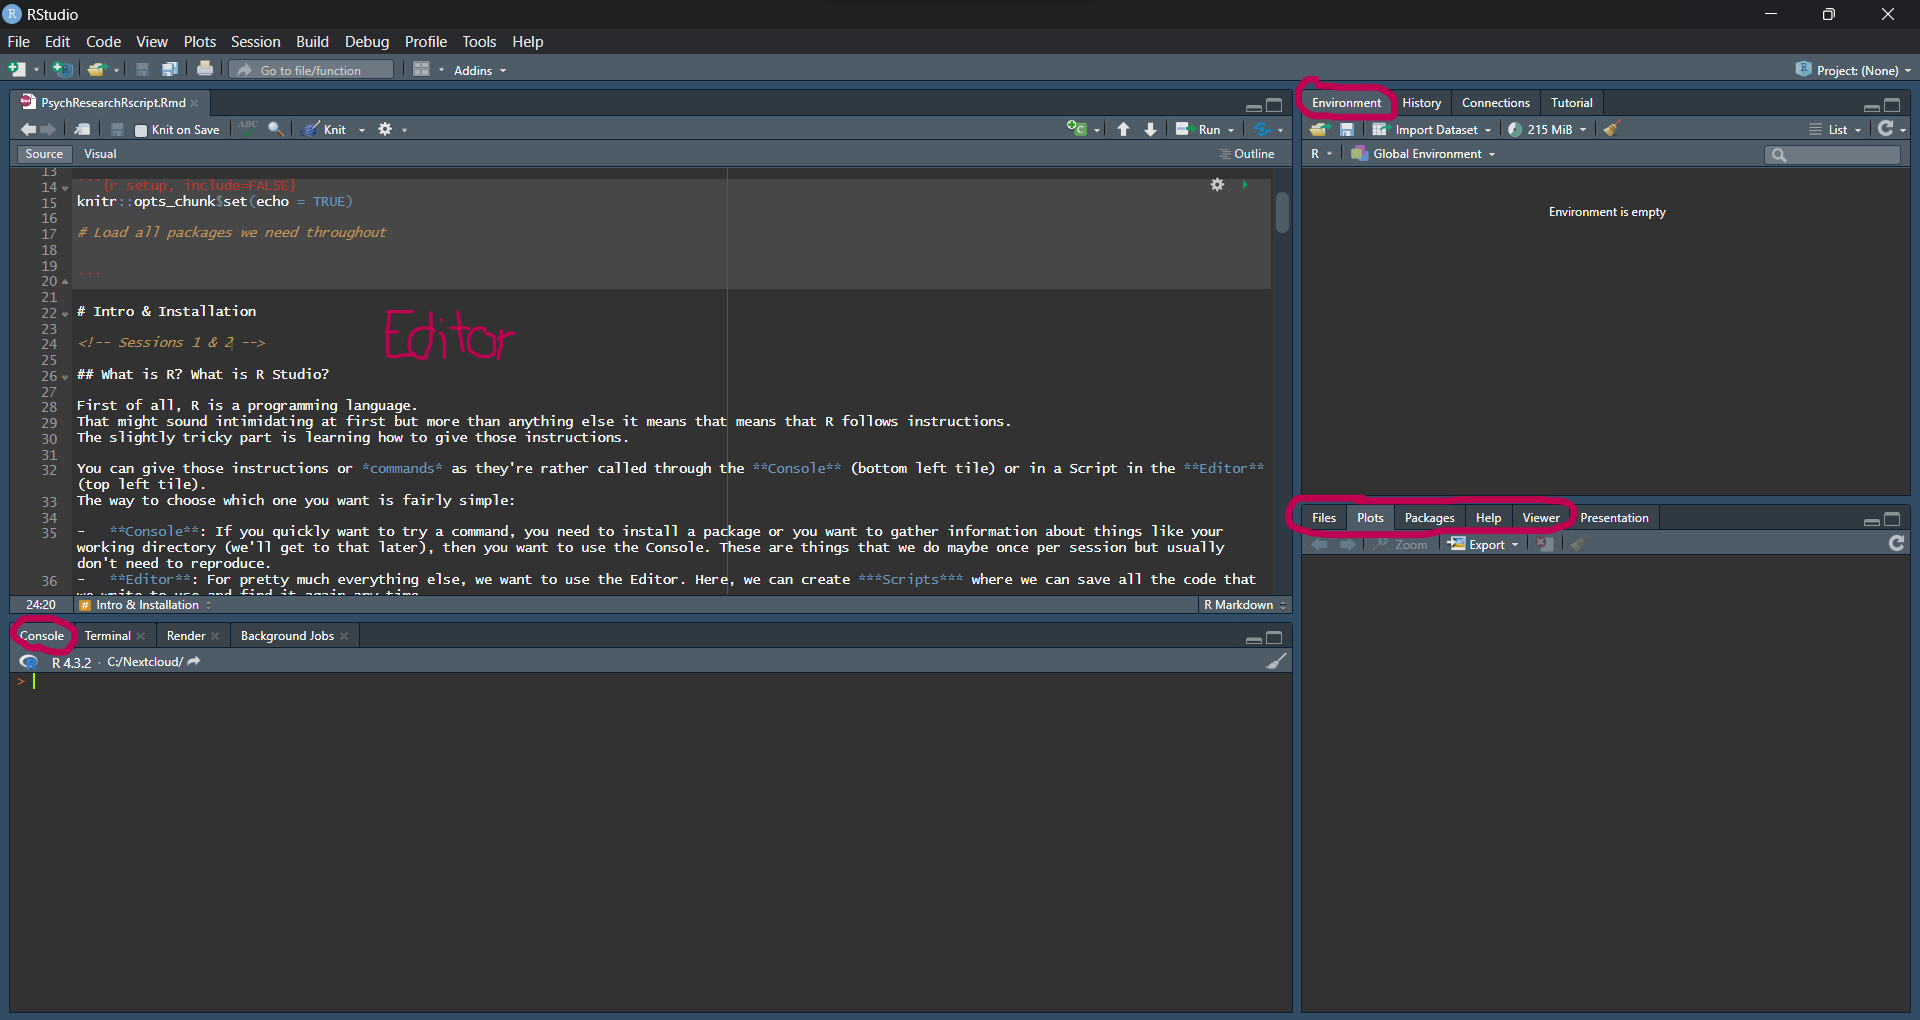
\includegraphics{./img/rstudio.png}
\caption{R Studio - typical layout}
\end{figure}

\section{Installing R and R Studio}\label{installing-r-and-r-studio}

\begin{itemize}
\tightlist
\item
  Download \& Install the newest R version 4.3.3 (2024-02-29 ucrt) at \url{https://cloud.r-project.org/}
\item
  Download and install R Studio at \url{https://posit.co/download/rstudio-desktop/}
\end{itemize}

R as a language can be used on its own.
However, it is not very modern, quite hard to use and frankly just no fun.
That's why we use R Studio as a user interface to run R.
Think of it as dipping your fingers in a pot of ink to write versus using a pen and paper - you will still write with the same ink, but the whole process is just nicer.

\subsection{Workflow}\label{workflow}

You can give instructions or \emph{commands} as they're rather called through the \textbf{Console} (bottom left tile) or in a Script in the \textbf{Editor} (top left tile).
The way to choose which one you want is fairly simple:

\begin{itemize}
\tightlist
\item
  \textbf{Console}: If you quickly want to try a command, you need to install a package or you want to gather information about things like your working directory (we'll get to that later), then you want to use the Console. These are things that we do maybe once per session but usually don't need to reproduce.
\item
  \textbf{Editor}: For pretty much everything else, we want to use the Editor. Here, we can create \textbf{\emph{Scripts}} where we can save all the code that we write to use and find again any time.
\end{itemize}

For most things - especially during the learning phase - it makes sense to write a Script in the Editor in order to be able to save and access the work.
To do so, simply click the 
\includegraphics[width=\textwidth,height=0.16667in]{./img/newfile.png} button and choose `R Script'.

Once we have a new script created, we can learn some basic things that R is capable of and save it to check out later.
Let's try to use R as a calculator first.
In the \emph{code chunk} below you will find some mathematical operations and their respective output.
Here as well as in other places that show R code (such as forums, blogs or help pages) you can recognize a code chunk by its gray background and mono space formatting.
Output is presented with the \texttt{{[}1{]}} at the start of the line.

\subsubsection*{Basic Math}\label{basic-math}
\addcontentsline{toc}{subsubsection}{Basic Math}

\begin{Shaded}
\begin{Highlighting}[]
\DecValTok{1}\SpecialCharTok{+}\DecValTok{2} 
\NormalTok{  [}\DecValTok{1}\NormalTok{] }\DecValTok{3}
\DecValTok{2{-}3}
\NormalTok{  [}\DecValTok{1}\NormalTok{] }\SpecialCharTok{{-}}\DecValTok{1}
\DecValTok{3}\SpecialCharTok{*}\DecValTok{4}
\NormalTok{  [}\DecValTok{1}\NormalTok{] }\DecValTok{12}
\DecValTok{4}\SpecialCharTok{/}\DecValTok{3}
\NormalTok{  [}\DecValTok{1}\NormalTok{] }\FloatTok{1.333333}
\DecValTok{5}\SpecialCharTok{\^{}}\DecValTok{2}
\NormalTok{  [}\DecValTok{1}\NormalTok{] }\DecValTok{25}
\end{Highlighting}
\end{Shaded}

\subsubsection*{Assigning Values}\label{assigning-values}
\addcontentsline{toc}{subsubsection}{Assigning Values}

\begin{Shaded}
\begin{Highlighting}[]
\NormalTok{a }\OtherTok{\textless{}{-}} \DecValTok{3}
\NormalTok{b }\OtherTok{\textless{}{-}} \DecValTok{4}
\NormalTok{a}\SpecialCharTok{{-}}\NormalTok{b}
\CommentTok{\# [1] {-}1}
\NormalTok{a}\SpecialCharTok{*}\NormalTok{b}\SpecialCharTok{+}\DecValTok{5}
\CommentTok{\# [1] 17}
\end{Highlighting}
\end{Shaded}

In these code chunks, R is essentially being used as a calculator to perform basic math.
While we want to make use of all the more powerful functions of R, it is important to grasp the basics and be able to use arithmetic for our purposes.
Next to the basic mathematical operators, there are many nifty mathematical functions, such as \texttt{sqrt()} - \emph{square root}, \texttt{sum()} or \texttt{pi}.

We also added \textbf{variables} containing values (here a and b hold values 3 and 4 respectively) that can be used in the calculations just like the values they contain.
As they only contain numbers, the variables a and b are called \textbf{numeric}.
We can check this property of a variable, e.g.~\texttt{a} using the function \texttt{class(a)}, which gives us ``numeric'' as output.

Usually when we fire up R, we don't just want to work with single values numeric but with \textbf{data frames} or \textbf{vectors} 
\includegraphics[width=\textwidth,height=0.20833in]{./img/vector.png} that can contain different classes of variables and several values respectively.

\subsubsection*{Vectors}\label{vectors}
\addcontentsline{toc}{subsubsection}{Vectors}

\begin{Shaded}
\begin{Highlighting}[]
\NormalTok{v }\OtherTok{\textless{}{-}} \FunctionTok{c}\NormalTok{(}\DecValTok{6}\NormalTok{, }\DecValTok{7}\NormalTok{, }\DecValTok{8}\NormalTok{)}
\FunctionTok{class}\NormalTok{(v)}
\CommentTok{\# [1] "numeric"}
\NormalTok{d }\OtherTok{\textless{}{-}} \FunctionTok{c}\NormalTok{(}\StringTok{"sunny"}\NormalTok{, }\StringTok{"rainy"}\NormalTok{, }\StringTok{"foggy"}\NormalTok{)}
\FunctionTok{class}\NormalTok{(d)}
\CommentTok{\# [1] "character"}
\end{Highlighting}
\end{Shaded}

\subsubsection*{Data Frame}\label{data-frame}
\addcontentsline{toc}{subsubsection}{Data Frame}

\begin{Shaded}
\begin{Highlighting}[]
\NormalTok{e }\OtherTok{\textless{}{-}} \FunctionTok{data.frame}\NormalTok{(v, d)}
\FunctionTok{class}\NormalTok{(e)}
\CommentTok{\# [1] "data.frame"}
\NormalTok{e}
\CommentTok{\#   v     d}
\CommentTok{\# 1 6 sunny}
\CommentTok{\# 2 7 rainy}
\CommentTok{\# 3 8 foggy}
\end{Highlighting}
\end{Shaded}

Notice that we did not just add all values one after the other, but followed a certain notation that begins with the function \texttt{c()}.
The c stands for ``combine'' or ``concatenate'' and tells R that all following values belong to the same variable.
There are several ways of adding variables to a data frame, but the \texttt{data.frame()} command is the simplest.

\begin{quote}
All values in a variable should have the same class.
Go ahead and try out \texttt{hm\ \textless{}-\ c(3,\ "sunny",\ 5.2)} and check the class.
What happened - did you expect that?
\end{quote}

When we have our data in a neat data frame, what we usually want to do is access either certain \textbf{rows} or \textbf{columns}.
To do so, base R uses square brackets \texttt{{[}{]}} behind the name of a data frame to indicate ``take this data, but only certain rows/columns/cells''.
Remember: The brackets understand the first input as rows and the second as columns - \emph{rows right away}.

\subsubsection*{Square Bracket Indexing}\label{square-bracket-indexing}
\addcontentsline{toc}{subsubsection}{Square Bracket Indexing}

\begin{Shaded}
\begin{Highlighting}[]
\NormalTok{e[}\DecValTok{1}\NormalTok{, ]}
\CommentTok{\#   v     d}
\CommentTok{\# 1 6 sunny}
\NormalTok{e[ , }\DecValTok{1}\NormalTok{]}
\CommentTok{\# [1] 6 7 8}

\NormalTok{weather }\OtherTok{\textless{}{-}}\NormalTok{ e[ , }\DecValTok{2}\NormalTok{]}
\NormalTok{weather}
\CommentTok{\# [1] "sunny" "rainy" "foggy"}

\NormalTok{e[}\DecValTok{1}\NormalTok{, }\DecValTok{1}\NormalTok{]}\SpecialCharTok{*}\NormalTok{e[}\DecValTok{2}\NormalTok{, }\DecValTok{1}\NormalTok{]}
\CommentTok{\# [1] 42}
\end{Highlighting}
\end{Shaded}

Our data set \texttt{e} contains three numbers in column c and different strings in column d.
We can select just the first row, or just the first column or either of the other rows and columns that we have in the data.
We can also re-assign the values, e.g.~to a new variable named ``weather'' or perform calculations on single cells in the data frame - only if they contain numerics, of course.

\begin{quote}
With square brackets we can only index rows and columns that are present in the data.
That maybe sounds obvious, but can easily lead to confusion because of error messages!
What happens when you try to index \texttt{e{[},3{]}}?
\end{quote}

While it is common practice to work with data frames and edit them according to our tasks and needs, using square brackets and base R can get a bit humdrum.
Luckily, many many people have developed many many packages that contain different functions, helping us in most tasks that we will need to tackle!

\section{Installing Packages}\label{installing-packages}

\begin{figure}
\centering
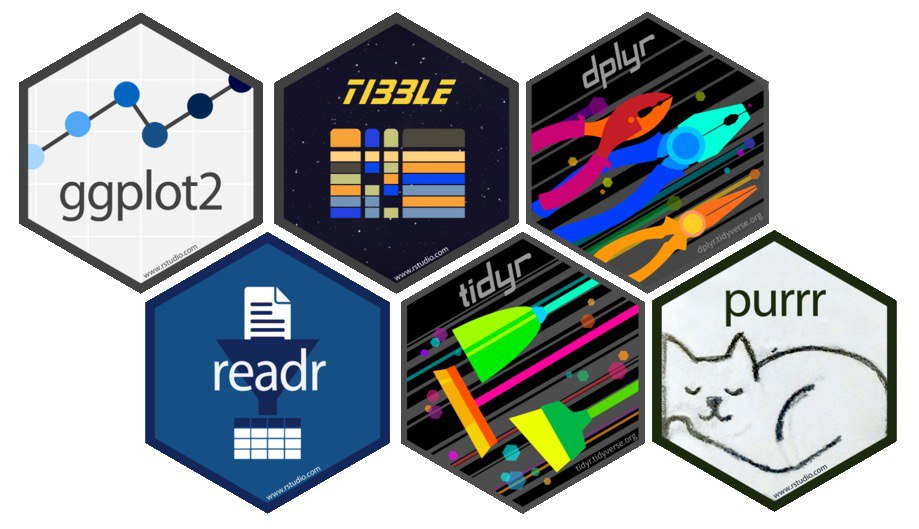
\includegraphics[width=\textwidth,height=0.625in]{./img/hexagons.png}
\caption{Hexagon Package logos}\label{id}
\end{figure}

Most packages are available on CRAN - the Comprehensive R Archive Network.
That being the case you can easily install the package you want to have with the command \texttt{install.packages("packagename")}.
It is important to note that the package name must be in quotes for the installation, while loading it into a script works without quotes using \texttt{library(packagename)}.

Packages usually serve quite specific purposes, e.g.~ones we will later get to know are \texttt{dplyr}, with which data handling is made a lot easier and more intuitive and \texttt{ggplot2}, which allows us to create beautiful, publication-ready plots and visualizations.
What is special about these two, among some others, is that they were developed by the same person (Hadley Wickham), and are made available in a sort of ``meta package'' - the \texttt{tidyverse}.
Installing and loading the \texttt{tidyverse} makes the functions from many different packages available at once.
This is quite convenient when we want to use a lot of those packages in the same session or script, but does also take a longer time to load and is sometimes not actually necessary.

To use this package of packages, please install the \texttt{tidyverse}, using \texttt{install.packages("tidyverse")} in the console and then load it into your script (or, again, directly in the console, bottom-left) with \texttt{library(tidyverse)}.
You can test whether it works by running \texttt{iris\ \%\textgreater{}\%\ pull(Sepal.Length)\ \%\textgreater{}\%\ mean()} in your console.
We will get to know the syntax in depth another time, but just so you know what's going on:
This line of code takes the data set \texttt{iris}, which is included in R by default, ``pulls'' the variable \texttt{Sepal.Length} out of the data and runs the \texttt{mean()} function on it, to calculate the average sepal length, which should be 5.8433333.

\section*{Wrap-Up \& Further Resources}\label{wrap-up-further-resources}
\addcontentsline{toc}{section}{Wrap-Up \& Further Resources}

R is a powerful language, R Studio is the user interface we use with it

R can be a calculator and perform basic and advanced math

We mostly work with variables and data frames

Packages make working with R easier and more fun!

\href{https://r-intro.tadaa-data.de/index.html}{Tadaa Data: R für Psychos (german)}

\href{https://www.kaggle.com/code/hamelg/intro-to-r-part-4-variables}{Kaggle: Intro to R}

\href{https://www.tidyverse.org/}{Tidyverse}

\chapter{R Basics \& Error Messages}\label{basics}

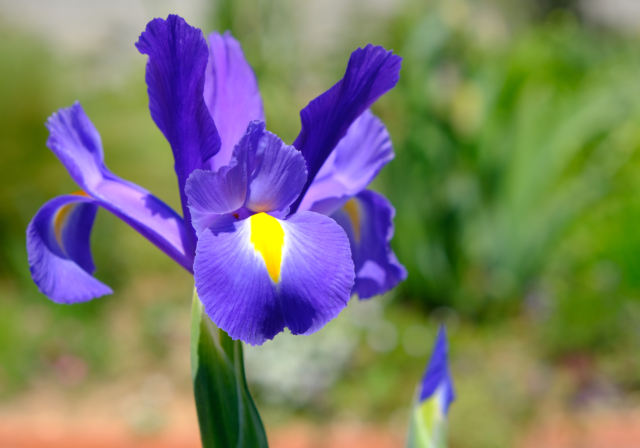
\includegraphics[width=\textwidth,height=1.5625in]{img/iris.png}

\section{Basics}\label{basics-1}

R is an object-based language.
The great advantage of that is we can assign values, vectors, text, matrices or almost anything else to variables and access them more easily later.
To do that, we use a left arrow \(\leftarrow\) like so:
\texttt{x\ \textless{}-\ c(1,\ 2,\ 3)}
Go ahead and try it out!
If you had too much fun assigning variables, you can remove them again from your work environment using the \texttt{rm()} command in the Console.
So, if you assign the values 1, 2 and 3 to \texttt{x}, you can type \texttt{rm(x)} into the console, hit enter and x has disappeared from your environment!

When you are working on a script, you can write and save all of your code.
You can also execute any line of code with \texttt{ctrl\ +\ enter} in the editor as you go along to test your code.
When you just want to run something once or test your code, you can enter it in the console where you just need to press \texttt{enter}/ \texttt{return}.

In your script, comments can and should be added to your code using the \texttt{\#}.
It is considered good practice to use comments generously, which will also help you to understand whats going on when you look at something a couple of days/weeks/years later and keep and overview!

\subsection*{Basic Functions}\label{basic-functions}
\addcontentsline{toc}{subsection}{Basic Functions}

Assign values \& look at a variable

\begin{Shaded}
\begin{Highlighting}[]
\NormalTok{a }\OtherTok{\textless{}{-}} \FunctionTok{c}\NormalTok{(}\DecValTok{1}\NormalTok{, }\DecValTok{2}\NormalTok{, }\DecValTok{3}\NormalTok{, }\DecValTok{4}\NormalTok{)}
\NormalTok{b }\OtherTok{\textless{}{-}} \FunctionTok{c}\NormalTok{(}\DecValTok{5}\NormalTok{, }\DecValTok{7}\NormalTok{, }\DecValTok{9}\NormalTok{, }\DecValTok{11}\NormalTok{)}
\NormalTok{a}
\CommentTok{\# [1] 1 2 3 4}
\end{Highlighting}
\end{Shaded}

Text aka \emph{strings} need to be put in quotes so it can be recognized as such

\begin{Shaded}
\begin{Highlighting}[]
\NormalTok{some\_text }\OtherTok{\textless{}{-}} \FunctionTok{c}\NormalTok{(}\StringTok{"amazing"}\NormalTok{, }\StringTok{"wow"}\NormalTok{)}
\end{Highlighting}
\end{Shaded}

Mean/average

\begin{Shaded}
\begin{Highlighting}[]
\FunctionTok{mean}\NormalTok{(a)}
\CommentTok{\# [1] 2.5}
\end{Highlighting}
\end{Shaded}

Standard deviation

\begin{Shaded}
\begin{Highlighting}[]
\FunctionTok{sd}\NormalTok{(b)}
\CommentTok{\# [1] 2.581989}
\end{Highlighting}
\end{Shaded}

Minimum

\begin{Shaded}
\begin{Highlighting}[]
\FunctionTok{min}\NormalTok{(b)}
\CommentTok{\# [1] 5}
\end{Highlighting}
\end{Shaded}

Maximum

\begin{Shaded}
\begin{Highlighting}[]
\FunctionTok{max}\NormalTok{(b)}
\CommentTok{\# [1] 11}
\end{Highlighting}
\end{Shaded}

Add values

\begin{Shaded}
\begin{Highlighting}[]
\NormalTok{a}\SpecialCharTok{+}\NormalTok{b}
\CommentTok{\# [1]  6  9 12 15}
\end{Highlighting}
\end{Shaded}

Find the sum of all values in a vector

\begin{Shaded}
\begin{Highlighting}[]
\FunctionTok{sum}\NormalTok{(b)}
\CommentTok{\# [1] 32}
\end{Highlighting}
\end{Shaded}

Find the length of a vector

\begin{Shaded}
\begin{Highlighting}[]
\FunctionTok{length}\NormalTok{(a)}
\CommentTok{\# [1] 4}
\end{Highlighting}
\end{Shaded}

Define a sequence

\begin{Shaded}
\begin{Highlighting}[]
\NormalTok{v }\OtherTok{\textless{}{-}} \DecValTok{3}\SpecialCharTok{:}\DecValTok{9}
\NormalTok{v}
\CommentTok{\# [1] 3 4 5 6 7 8 9}
\end{Highlighting}
\end{Shaded}

Find the range of a vector

\begin{Shaded}
\begin{Highlighting}[]
\FunctionTok{range}\NormalTok{(v)}
\CommentTok{\# [1] 3 9}
\end{Highlighting}
\end{Shaded}

Define several sequences in one vector

\begin{Shaded}
\begin{Highlighting}[]
\NormalTok{d }\OtherTok{\textless{}{-}} \FunctionTok{c}\NormalTok{(}\DecValTok{10}\SpecialCharTok{:}\DecValTok{15}\NormalTok{, }\DecValTok{20}\SpecialCharTok{:}\DecValTok{25}\NormalTok{)}
\NormalTok{d}
\CommentTok{\#  [1] 10 11 12 13 14 15 20 21 22 23 24 25}
\end{Highlighting}
\end{Shaded}

Now that we know how to assign values and how to find some basic stats on single vectors, we will look at how to extract specific values from vectors.
We call this indexing and in R we can use square brackets to do so.

Find the first value in a vector

\begin{Shaded}
\begin{Highlighting}[]
\NormalTok{d[}\DecValTok{1}\NormalTok{]}
\CommentTok{\# [1] 10}
\end{Highlighting}
\end{Shaded}

Find the value where a vector has a specific value - this is especially interesting when we want to compare two vectors

\begin{Shaded}
\begin{Highlighting}[]
\NormalTok{d[d}\SpecialCharTok{==}\DecValTok{10}\NormalTok{]}
\CommentTok{\# [1] 10}
\NormalTok{a[d}\SpecialCharTok{==}\DecValTok{10}\NormalTok{]}
\CommentTok{\# [1] 1}
\end{Highlighting}
\end{Shaded}

Less convoluted: Find the index where a vector has a specific value

\begin{Shaded}
\begin{Highlighting}[]
\FunctionTok{which}\NormalTok{(d}\SpecialCharTok{==}\DecValTok{12}\NormalTok{)}
\CommentTok{\# [1] 3}
\end{Highlighting}
\end{Shaded}

You can practice these functions on your own and definitely check out the \hyperref[exercises]{Exercises} section!

\begin{quote}
\textbf{Brainteaser} :
We define two variables in the following way:

\begin{Shaded}
\begin{Highlighting}[]
\NormalTok{e }\OtherTok{\textless{}{-}} \DecValTok{1}\SpecialCharTok{:}\DecValTok{5}
\NormalTok{f }\OtherTok{\textless{}{-}} \DecValTok{2}\SpecialCharTok{:}\DecValTok{5}
\end{Highlighting}
\end{Shaded}

Let's say we want to access the number 5 in both variables.
How come \texttt{e{[}5{]}} works but \texttt{f{[}5{]}} does not?
\end{quote}

Now, you may be wondering why I skipped the letter c and whether you should be taking the word of someone who clearly does not know their ABCs.
The reason is quite simple: You already saw the function \texttt{c()} in the last chapter, which is used to create variables that are larger than one entry\footnote{Technically, that is also not true as you just saw that we can create continuous sequences with a colon, i.e.~\texttt{1:3} is 1, 2, 3.}.
It stands for combine and it was used in the code above to create the variable \texttt{d}, containing two sequences.
So, while you can use single letters as variable names for placeholders, it is generally not a great idea to use \texttt{c} - if we can avoid confusing for ourselves, we want to do it.
There is a whole section on how to name your variables in Section \ref{varnames} so that future-you won't be mad.

\section{Logic}\label{logic}

Next to numeric variables like \texttt{a} and \texttt{b} that hold numbers, and string variables that hold \texttt{"text"}, there are also so-called \emph{boolean} variables.
They can only hold the values \textbf{TRUE} or \textbf{FALSE} and are either assigned specifically by you, the user, or result from basically asking R a yes-or-no question.
For example:

Is 3 smaller than 7?

\begin{Shaded}
\begin{Highlighting}[]
\DecValTok{3} \SpecialCharTok{\textless{}} \DecValTok{7}
\CommentTok{\# [1] TRUE}
\end{Highlighting}
\end{Shaded}

Is 3 smaller than 2?

\begin{Shaded}
\begin{Highlighting}[]
\DecValTok{3} \SpecialCharTok{\textless{}} \DecValTok{2}
\CommentTok{\# [1] FALSE}
\end{Highlighting}
\end{Shaded}

Now, these examples are fairly trivial but boolean variables using logic can be really helpful, e.g.~for filtering data.
You can find the mean of some variable for a specific group by telling R your criteria and the operation you want to conduct on the filtered data.
Let's say we asked some students about their gender and their skills with R.
If we want to know the average R skills of male students we would tell R: ``If the gender of a participant is male, include them in the mean value for R skill''.
So our code would look something like this:

\begin{Shaded}
\begin{Highlighting}[]
\NormalTok{mean\_r\_skill\_m }\OtherTok{\textless{}{-}} \FunctionTok{mean}\NormalTok{(data}\SpecialCharTok{$}\NormalTok{r\_skill[data}\SpecialCharTok{$}\NormalTok{gender }\SpecialCharTok{==} \StringTok{"male"}\NormalTok{])}
\end{Highlighting}
\end{Shaded}

Of course, if you try to run this code you will probably encounter one of the errors described in the next section, because we do not currently have a dataset called \texttt{data}.
But you can try out the principle with one of the \hyperref[exercises]{Exercises}!
Depending on the analysis you need, you can use any of these so-called ``logic operators'':

\begin{Shaded}
\begin{Highlighting}[]
\NormalTok{x }\OtherTok{\textless{}{-}} \DecValTok{4}\NormalTok{; y }\OtherTok{\textless{}{-}} \DecValTok{5}
\NormalTok{x }\SpecialCharTok{\textless{}}\NormalTok{ y }\CommentTok{\# smaller than}
\CommentTok{\# [1] TRUE}
\NormalTok{x }\SpecialCharTok{\textless{}=} \DecValTok{4} \CommentTok{\# smaller/ equal}
\CommentTok{\# [1] TRUE}
\NormalTok{x }\SpecialCharTok{\textgreater{}}\NormalTok{ y }\CommentTok{\# greater than}
\CommentTok{\# [1] FALSE}
\NormalTok{x }\SpecialCharTok{\textgreater{}=} \DecValTok{3} \CommentTok{\# greater/ equal}
\CommentTok{\# [1] TRUE}
\end{Highlighting}
\end{Shaded}

\begin{Shaded}
\begin{Highlighting}[]
\NormalTok{x }\SpecialCharTok{==}\NormalTok{ y }\CommentTok{\# equal to}
\CommentTok{\# [1] FALSE}
\NormalTok{x }\SpecialCharTok{!=}\NormalTok{ y }\CommentTok{\# not equal to}
\CommentTok{\# [1] TRUE}
\NormalTok{z }\OtherTok{\textless{}{-}} \ConstantTok{TRUE}
\NormalTok{z}
\CommentTok{\# [1] TRUE}
\SpecialCharTok{!}\NormalTok{z}
\CommentTok{\# [1] FALSE}
\end{Highlighting}
\end{Shaded}

You can find a concise overview over all of these operators in the \hyperref[toolbox]{Toolbox}.

\section{Reading Error Messages}\label{reading-error-messages}

Even the most advanced R coder will encounter the occasional error message.
While they are quite helpful and usually lead to being able to solve problems, it can be challenging to learn how to properly read the message in order to actually understand what the problem is.
Therefore, we will look at some of the most common wordings to decipher what R needs so it can understand what we want to do.

Think of error messages not as discouraging faults of your program but rather as invites to help you help R understand what you are trying to achieve.

\subsection*{\texorpdfstring{\emph{Error: unexpected `X' in ``Y''}}{Error: unexpected `X' in ``Y''}}\label{error-unexpected-x-in-y}
\addcontentsline{toc}{subsection}{\emph{Error: unexpected `X' in ``Y''}}

This message is fairly straightforward:
R expected a certain kind of symbol at the place where we put `X' and is now confused because our input did not match the expectation.

For most Europeans, for example, the most commonly used decimal separator will be a comma.
Since R is an american-built language, however, it expects decimals to be separated with a decimal point while commas indicate separate inputs to a function.
Therefore, when we accidentally input a decimal as `3,141', we will receive the error message \emph{Error: unexpected `,' in ``3,''} because R expected the input to be something like `3.141'.

\textbf{Fix: Replace the `x' in ``Y'' with something that R can understand.} Or alternatively: Make sure that we meant the input like that.

\subsection*{\texorpdfstring{\emph{Error: object `A' not found}}{Error: object `A' not found}}\label{error-object-a-not-found}
\addcontentsline{toc}{subsection}{\emph{Error: object `A' not found}}

This, too, is pretty understandable message:
The object that you are trying to access and use cannot be found by R.
The most common cause for this error message is probably simply that you misspelled the object name somewhere.
R is case-sensitive, so maybe object \emph{A} was defined as object \emph{a}?
Maybe the object \emph{vector} is spelled \emph{vcteor} in your function?

Moreover, sometimes our thoughts are two steps ahead of our code.
When figuring out how to get a program to work, sometimes we presume that a variable exists just because we need it and forget to define the variable up front.
The same goes if we try to access a variable in a data frame that was maybe defined in a different data frame or as its own vector - it simply cannot be found because we are having R look in the wrong place.

\textbf{Fix: Make sure the object name is spelled correctly and was defined prior to using it in a function, calculation or elsewhere.}

This error message also often appears with ``function xyz not found''.
In this case, we probably forgot to load the package first, which contains that function.
Thus, the fix will likely be to figure out which package contains the function we are trying to use and load it with the \texttt{library()} command.

\subsection*{\texorpdfstring{\emph{Error}: R does nothing after running a command}{Error: R does nothing after running a command}}\label{error-r-does-nothing-after-running-a-command}
\addcontentsline{toc}{subsection}{\emph{Error}: R does nothing after running a command}

This is not an error message but it is still very common, especially at the beginning of your learning journey.
Usually, there is a \texttt{\textgreater{}} symbol at the beginning of your console input line, which indicates that R is ready to run some code.
However, if R is ``unfinished'' with a command, you see a \texttt{+} instead.
This happens when R can`t work with the command because there is something missing, which in most cases, will be a closing parenthesis.

\textbf{Fix: Click in your console and use the \texttt{Esc} button to cancel the command. Then, look at the code you were trying to run and see if there is some closing statement such as \texttt{)} missing and try again.}

\subsection*{\texorpdfstring{The pipe operator \texttt{\textbar{}\textgreater{}} or \texttt{\%\textgreater{}\%}}{The pipe operator \textbar\textgreater{} or \%\textgreater\%}}\label{pipe1}
\addcontentsline{toc}{subsection}{The pipe operator \texttt{\textbar{}\textgreater{}} or \texttt{\%\textgreater{}\%}}

Next to missing closing parentheses, a classic source for this behavior is the so-called pipe operator, created with either \texttt{\textbar{}\textgreater{}} (native R pipe, available since R version 4.1.0) or \texttt{\%\textgreater{}\%} (tidyverse pipe from the \texttt{magrittr} package).
It will be used a lot starting in Chapter \ref{dplyr} and it is probably one of my personal favorite R features.
The pipe allows you to use previous operations in the next one easily and clearly.
In reality this relates to not drowning in parenthesis and everything in the \texttt{tidyverse} is designed to be used with a pipe.

Let me show you what I mean: We will create a variable that contains some numbers and we want to find the average value rounded to two decimal spaces.
We already know the \texttt{mean()} function; to round a number we use the \texttt{round()} function and define how many decimal places to round to after we input the value we want to round.

\begin{Shaded}
\begin{Highlighting}[]
\CommentTok{\# Code without pipe}
\FunctionTok{round}\NormalTok{(}\FunctionTok{mean}\NormalTok{(}\FunctionTok{c}\NormalTok{(}\DecValTok{5}\NormalTok{, }\DecValTok{9}\NormalTok{, }\DecValTok{2}\NormalTok{)), }\DecValTok{2}\NormalTok{)}
\CommentTok{\# [1] 5.33}

\CommentTok{\# Code with pipe}
\FunctionTok{c}\NormalTok{(}\DecValTok{5}\NormalTok{, }\DecValTok{9}\NormalTok{, }\DecValTok{2}\NormalTok{) }\SpecialCharTok{|\textgreater{}} \FunctionTok{mean}\NormalTok{() }\SpecialCharTok{|\textgreater{}} \FunctionTok{round}\NormalTok{(}\DecValTok{2}\NormalTok{)}
\CommentTok{\# [1] 5.33}
\end{Highlighting}
\end{Shaded}

As you can see, both lines of code will give the same result but the pipeline follows a much more intuitive way of coding and allows you to write your code as you would think of the analysis.
As opposed to that, in the first line you need to first think of rounding, then of the mean and then last input your actual values, which seems very backwards.
Also, as I mentioned, you can see that there are already some parentheses next to each other, which would be really easy to forget and not receive any output.

Generally, I wholeheartedly recommend getting familiar with piping very early on when learning R.
However, don't forget that R expects input after each pipe.
If you accidentally end a line of code with a pipe, you will encounter the behavior where R just does nothing and you basically have a staring battle of who will give in first.
The same fix will work here: Hit the Esc button, look at the code you were trying to run and figure out if there might have been a pipe that just went nowhere.

\begin{quote}
When you need help figuring out how a function works, there are several ways to get it. Try typing \textbf{?``\textbar\textgreater{}'' } into your console and hit enter!
\end{quote}

\begin{Shaded}
\begin{Highlighting}[]
\NormalTok{knitr}\SpecialCharTok{::}\FunctionTok{include\_url}\NormalTok{(}\StringTok{"./img/nerfect.webp"}\NormalTok{)}
\end{Highlighting}
\end{Shaded}

So, always keep in mind: Mistakes happen to everyone.
Error messages can be really frustrating but they really are meant to be helpful.
Sometimes R has a hard time understanding what's wrong, so if an error message seems vague, think of it as your chance to play detective and figure out what happened.
Also, I promise you that mastering the art of reading error messages can be tedious, but it is very worth it.
Once you get a feeling of how R tries to identify errors, it gets a lot less disheartening.
It can actually be quite wholesome to see a big, intimidating error message that makes absolutely no sense at all, just to find a teeny, tiny typo in your code which works once you fix it.

\section*{Exercises}\label{exercises}
\addcontentsline{toc}{section}{Exercises}

\textbf{\emph{Logic}}

We want to find out whether the average Petal Length and Sepal Length of iris flowers are different from each other.

Use what you know to ``ask R'' if those values are unequal!

Hint: You will need logic, the mean()-function and square brackets. Use \textbf{names(iris)} to find all variable names in that data set.

Solution

\begin{itemize}
\tightlist
\item
  Square bracket indexing with the variable name in quotes \newline
  \texttt{iris{[}\ ,\ "Sepal.Length"{]}}\\
  \texttt{iris{[}\ ,\ "Petal.Length"{]}}
\item
  now we add the mean function around both like this:
  \texttt{mean(iris{[}\ ,\ "Sepal.Length"{]})}\\
  \texttt{mean(iris{[}\ ,\ "Sepal.Length"{]})}
\item
  Finally we compare the two with the != operator:
  \texttt{mean(iris{[}\ ,\ "Sepal.Length"{]})\ !=}
  \texttt{mean(iris{[}\ ,\ "Petal.Length"{]})}\\
  TRUE
\end{itemize}

\textbf{\emph{Create a vector}}

Create a vector x with the numbers from 50 to 100 and 150 to 200.

Find its mean, standard deviation and its range.

What is the 77th number of vector x?

Solution

\begin{itemize}
\tightlist
\item
  \texttt{x\ \textless{}-\ c(50:100,\ 150:200)}\strut \\
\item
  \texttt{mean(x),\ sd(x),\ range(x)\ \%\textgreater{}\%\ round(2)}: \newline 125, 52.38, 50, 200

  \begin{itemize}
  \tightlist
  \item
    \texttt{\%\textgreater{}\%\ round(2)} takes the numbers and rounds them up to two decimal points
  \end{itemize}
\item
  \texttt{x{[}77{]}}: 175
\end{itemize}

\textbf{\emph{Code with problems}}

Below is some code that has a few problems.

Try to identify them and how they might be fixed. Feel free to test them out if you are not sure!

\texttt{Library(greatpackage)}

Solution

\begin{itemize}
\tightlist
\item
  \texttt{library} should not be capitalized
\item
  ``greatpackage'' does not exist and can thus not be loaded
\end{itemize}

\texttt{mean(coolvariable)}

Solution

coolvariable was not defined previously

\texttt{a\ \textless{}-\ c(1,\ 3,\ 6,\ 7}

Solution

the command is not finished, it needs a closing parentheses

\texttt{b\ \textless{}-\ c(2,\ 4;\ 6,\ 8)}

Solution

we need all commas to separate numbers in a vector, not a semicolon

\section*{Wrap-Up \& Further Resources}\label{wrap-up-further-resources-1}
\addcontentsline{toc}{section}{Wrap-Up \& Further Resources}

Functions work with input inside round brackets, e.g.~c(1, 2, 3)

a point \textbf{.} is a decimal separator in numbers; a comma \textbf{,} seperates input in functions

Logical operators compare data, e.g.~7 \textgreater{} 6 would output TRUE

\texttt{\#} allows comments in the code

Errors should be invitations to make your code more understandable for R

\(\rightarrow\) the better we understand the problem, the better we can fix it!

\href{https://stackoverflow.com/}{StackOverflow}

\href{https://katalog.uni-konstanz.de/libero/WebOpac.cls?VERSION=2&ACTION=DISPLAY&RSN=2222774&DATA=KON&TOKEN=nGIfSiZsIA5826&Z=1&SET=1}{Discovering Statistics Using R} Book by Andy Field, available from KIM

\chapter{Best Practice}\label{best-practice}

\begin{quote}
'' \st{All} Many roads lead to Rome''
\end{quote}

You can achieve most things in many different ways - \emph{best practice} refers to the best/ easiest/ clearest way of working with R.
Some of the things you will read about might not make sense to you intuitively and that's ok.
Realistically, there are some mistakes that everyone must make for themselves.
When you do, I just want you to remember that here is some advice that you have either heard before or will read up on now to get out of the pickle you may be in!
Maybe you would like to bookmark the \hyperref[toolbox]{toolbox} to always find an overview of nifty tips, tricks and hacks?

\section{Naming Conventions}\label{varnames}

R is a so-called \emph{object-oriented} language.
What that means for us is mostly that all our data exist as ``objects'' as far is R is concerned.
Just like in real life, we can \emph{do} stuff with those objects now, which is called using a \emph{function} or \emph{command}.
Which brings me to the importance of proper names for all your variables, data sets, functions\ldots{}
Everything.

If we go to the market and I tell you to get me an apple, you will probably be confused if there are many types of apples, maybe different colors, maybe different breeds.
Basically, if I don't specify which apple I want, you are not able to pick out the right one.
The same is true for R: If you try to call a function but fail to specify what object to use the function on, R is confused and throws you an error.

Now, this may seem pretty obvious but it is a pretty common source of errors, especially during the ``steep phase'' of the learning curve.
In R, \texttt{abc} is a different object than \texttt{ABC}, which is different from \texttt{a\_b\_c}, which is different from \texttt{A.B.C}. All of these variants are possible ways of naming your objects in R.
However, it makes everyone's life significantly easier to stick to some naming-guidelines.

\begin{itemize}
\tightlist
\item
  Preferably use \textbf{lower-case} variable names, e.g.~\texttt{gender} instead of \texttt{Gender} or \texttt{GENDER}.
\item
  Preferably use an \textbf{underscore} to differentiate between different words in your object names if necessary, e.g.~\texttt{music\_preference}.
\item
  \textbf{Avoid using numbers} in your names because likely either you or R will get confused with this at some point, e.g.~\texttt{raw\_data} instead of \texttt{data1}\footnote{Additionally, the 1 (one) and the l (lower-case L) can look very similar, which makes thing just even worse when trying to figure out an error.}.
\item
  Use \textbf{abbreviations} where useful, e.g.~\texttt{rt} instead of \texttt{reaction\_times}.
\item
  Use \textbf{names that will still make sense} to you in the future, i.e.~avoid names like \texttt{asdf\_data} or \texttt{blibblobfundata}. The best case scenario would be that your variable names also makes sense to other people if they try to understand your code!
\end{itemize}

I will admit that some of these pieces of advice are more opinionated personal experience than objective facts.
The more you work with variables and maybe also code from other people, you may form your own opinions on what the best naming conventions are for you.
I strongly suggest finding a way that works for you and sticking with it.
As I described above, I personally will try to stick to \emph{lower\_snake\_case} to name my variables because it is usually very clear, easy to read by humans and computers and would also be usable in any other programming language.

Another thing that can take some time to get used to is avoiding white spaces in file names and any other names, for that matter.
R has problems finding files with names such as ``My file with a really specific name.bib'', which can easily be avoided by sticking to snake\_case: ``My\_file\_with\_a\_really\_specific\_name.bib''.
The same goes for variables: In my first class, we discovered that it is possible in R to set a variable name with a space.
Just because it's possible does not mean anybody should do it. Ever.

You can try it out: Enter \texttt{"hi\ there"\ \textless{}-\ 5} in your console to assign the value 5 to a variable named \texttt{hi\ there}.
You will see it appear in your working environment, but accessing the variable is virtually impossible.
If you just type \texttt{hi\ there} in the console and hit Enter, R will give you an error à la \emph{``unexpected symbol''}.
But if you type \texttt{"hi\ there"}, it will echo the text back to you.

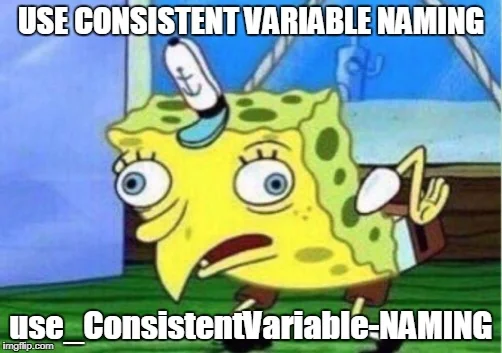
\includegraphics[width=\textwidth,height=2.08333in]{./img/varname.png}

\url{https://www.reddit.com/r/ProgrammerHumor/comments/6stwag/can_you_stick_to_any_naming_convention/}

Here is a list of positive and negative naming examples:

\begin{itemize}
\tightlist
\item
  \texttt{great\ variable}

  \begin{itemize}
  \tightlist
  \item
    Spaces can technically work but are a hassle to access
  \end{itemize}
\item
  \texttt{Areallysuperinsanelyverylongvariablename}

  \begin{itemize}
  \tightlist
  \item
    Variables are supposed to \emph{reduce} workload
  \end{itemize}
\item
  \texttt{Howaboutthis\$}

  \begin{itemize}
  \tightlist
  \item
    Special characters should be avoided
  \end{itemize}
\item
  \texttt{age\_grouped}

  \begin{itemize}
  \tightlist
  \item
  \end{itemize}
\item
  \texttt{GenderRecoded}

  \begin{itemize}
  \tightlist
  \item
  \end{itemize}
\item
  \texttt{aMAZING¯vARIABLE¯nAME}

  \begin{itemize}
  \tightlist
  \item
    Please just no.
  \end{itemize}
\end{itemize}

\section{Exercise: Creating Data}\label{exercise-creating-data}

Imagine we are going to measure some test scores at a school that are supposed to reflect the kids' IQ (mean 100, sd 15).
In order to prepare for data analysis, we want to simulate what the data might look like beforehand.

We are going to measure their age and IQ score and we will be assessing class 7a and 7b.

Create \textbf{two data frames} - one for each class.
They should each contain \textbf{n = 20 entries} (for 20 kids) and \textbf{2 variables i.e.~age and IQ score}.
We assume \textbf{age is a random number from 12 to 15} and \textbf{IQ follows normal distribution with mean = 100, sd = 15}.

Afterwards, add a variable to code the \textbf{class} to each data frame and add them together \textbf{underneath each other}.

Which functions should I use?

The functions you will need are \emph{data.frame, sample, rnorm, \$, rbind} and \emph{str}.
You can read help on any function by typing a question mark before the function name in your console and hitting Enter, e.g.~\texttt{?rnorm}.

Solution

\begin{Shaded}
\begin{Highlighting}[]
\CommentTok{\# Create the data frames}
\NormalTok{scores7a }\OtherTok{\textless{}{-}} \FunctionTok{data.frame}\NormalTok{(}\AttributeTok{age =} \FunctionTok{sample}\NormalTok{(}\AttributeTok{x =} \DecValTok{12}\SpecialCharTok{:}\DecValTok{15}\NormalTok{, }\AttributeTok{size =} \DecValTok{20}\NormalTok{, }\AttributeTok{replace =}\NormalTok{ T),}
                       \AttributeTok{iq =} \FunctionTok{rnorm}\NormalTok{(}\AttributeTok{n =} \DecValTok{20}\NormalTok{, }\AttributeTok{mean =} \DecValTok{100}\NormalTok{, }\AttributeTok{sd =} \DecValTok{15}\NormalTok{))}

\NormalTok{scores7b }\OtherTok{\textless{}{-}} \FunctionTok{data.frame}\NormalTok{(}\AttributeTok{age =} \FunctionTok{sample}\NormalTok{(}\AttributeTok{x =} \DecValTok{12}\SpecialCharTok{:}\DecValTok{15}\NormalTok{, }\AttributeTok{size =} \DecValTok{20}\NormalTok{, }\AttributeTok{replace =}\NormalTok{ T),}
                       \AttributeTok{iq =} \FunctionTok{rnorm}\NormalTok{(}\AttributeTok{n =} \DecValTok{20}\NormalTok{, }\AttributeTok{mean =} \DecValTok{100}\NormalTok{, }\AttributeTok{sd =} \DecValTok{15}\NormalTok{))}
\CommentTok{\# Notice anything about the code?}

\FunctionTok{str}\NormalTok{(scores7a); }\FunctionTok{str}\NormalTok{(scores7b)}
\CommentTok{\# \textquotesingle{}data.frame\textquotesingle{}: 20 obs. of  2 variables:}
\CommentTok{\#  $ age: int  15 12 12 12 12 14 15 13 15 12 ...}
\CommentTok{\#  $ iq : num  95.3 94.2 79.1 125.2 87.7 ...}
\CommentTok{\# \textquotesingle{}data.frame\textquotesingle{}: 20 obs. of  2 variables:}
\CommentTok{\#  $ age: int  14 14 14 15 13 13 15 13 12 12 ...}
\CommentTok{\#  $ iq : num  78.9 97.3 114.4 96.5 96.1 ...}

\CommentTok{\# Add information about the class}
\NormalTok{scores7a}\SpecialCharTok{$}\NormalTok{class }\OtherTok{\textless{}{-}} \StringTok{"7a"}
\NormalTok{scores7b}\SpecialCharTok{$}\NormalTok{class }\OtherTok{\textless{}{-}} \StringTok{"7b"}

\CommentTok{\# create big dataframe}
\NormalTok{allscores }\OtherTok{\textless{}{-}} \FunctionTok{rbind}\NormalTok{(scores7a, scores7b)}

\CommentTok{\# Check the overall data frame for plausibility}
\FunctionTok{str}\NormalTok{(allscores)}
\CommentTok{\# \textquotesingle{}data.frame\textquotesingle{}: 40 obs. of  3 variables:}
\CommentTok{\#  $ age  : int  15 12 12 12 12 14 15 13 15 12 ...}
\CommentTok{\#  $ iq   : num  95.3 94.2 79.1 125.2 87.7 ...}
\CommentTok{\#  $ class: chr  "7a" "7a" "7a" "7a" ...}
\FunctionTok{table}\NormalTok{(allscores}\SpecialCharTok{$}\NormalTok{class)}
\CommentTok{\# }
\CommentTok{\# 7a 7b }
\CommentTok{\# 20 20}
\end{Highlighting}
\end{Shaded}

\section{Working Directories}\label{working-directories}

A working directory corresponds to the folder on your computer that you are \textbf{working in}.
It is similar to when you open up a program such as Word and then locate a file that you wish to open there - you need to find the folder on your machine where that file is located.
With R, we usually either just open up R Studio or we will directly open a script.
Commonly, the working directory will either be the default folder (e.g.~``Documents'' on Windows) or if you open up a script from a specific location, it might also be set to that folder automatically.
Vice versa, if you work on a script in R Studio and save it, it will saved in the folder that is currently set as the working directory.

You can check your current working directory by entering \texttt{getwd()} in the console.
It will output a so-called file path that ``explains'' which folder your are working in.
In the default view of R Studio you can also find the ``Files'' tab in the lower right corner and it will show the contents of your current working directory.
If you want to change the working directory you can use the command \texttt{setwd()} and enter a file path in the parentheses.

\begin{quote}
Try it out: Execute the getwd() command in the console.
Which folder is R working in - is it the one you expected?
\end{quote}

While this way of structuring your work in folders and directories is very common, it can pose some issues down the line.
Usually, we will work with our own data files (see Chapter @ref(\#exdata)) and read them into our script to use them for analyses.
If they happen to be in a different folder than our working directory, we will need to use the complete file path to tell R where to find this data file.
When we now ask someone else to try out the code - either because we need help or because we are handing in an assignment - they will raise an eyebrow because chances are that they do not have the specified file path available on their machine.

\begin{quote}
{[}1{]} ``C:/Users/Tave/great\_projects/my\_specific\_folder\_name''
\end{quote}

The same goes for us if we ever want to use a different machine, e.g.~for work.
Moreover, it is quite easy to forget which folder you are currently working in, which means it can get hard to later locate your scripts again.

This may all sound like quite the hassle, but luckily there is a simple solution built right into R Studio that will make self-organization easy.

\section[R Projects ]{\texorpdfstring{R Projects \protect
\includegraphics[width=\textwidth,height=0.3125in]{./img/rproj.png}}{R Projects R Project}}\label{r-projects-r-project}

A project in R is essentially a bookmark to a specific folder on your computer.
It lets you organize your projects very clearly, so you can e.g.~create a folder for your thesis where you save the data you collected and the R scripts to wrangle that data.
When you open the R project it automatically sets your working directory to the folder you put the project in.
It also makes it easier for you to use so-called \emph{relative file paths}, allowing you not to specify a full file path when you want to reference a data file or maybe a BibTex file that contains citations for a paper or thesis.
With a relative file path you can use a period as a placeholder for ``current folder/working directory'' and then just specify the path from there.

\begin{quote}
Let's try that out under \texttt{File} \(\rightarrow\) \texttt{New\ project...}
\end{quote}

This is also great for sharing your code and projects:
If someone else has the same data file in their R project then they will be able to use your scripts containing just the relative path and be able to execute the code.

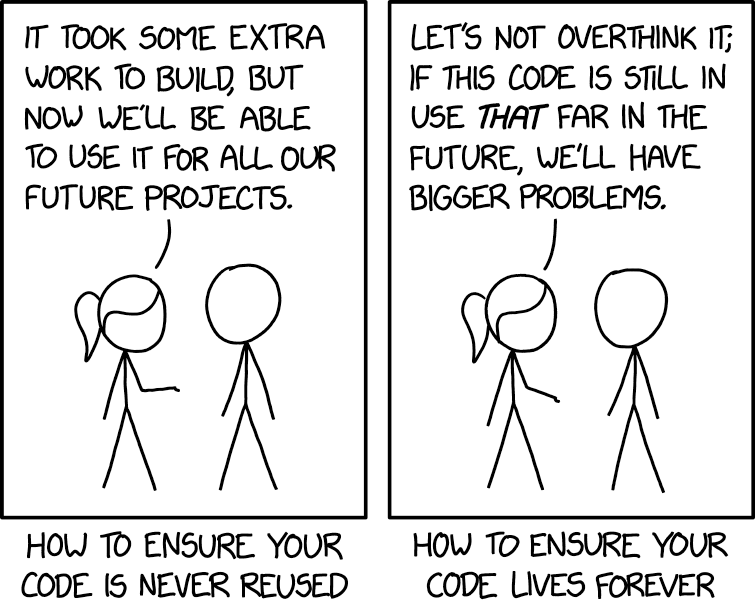
\includegraphics[width=\textwidth,height=2.08333in]{./img/code_lifespan.png}

\url{https://xkcd.com/2730/}

Next to all advantages with sharing as well as creating reproducible code, working with R projects will also help you in keeping your workflow organized.
In the following, you can try to create your own R project and see how to use the relative file path!

\subsection*{Exercise}\label{exercise}
\addcontentsline{toc}{subsection}{Exercise}

\begin{enumerate}
\def\labelenumi{\arabic{enumi}.}
\tightlist
\item
  Create a subfolder called ``data'' in your R project.
\item
  Download the file ``mindfulness\_data.Rds'' from \href{https://github.com/the-tave/psych_research_in_r/blob/main/data/mindfulness_data.Rds}{GitHub} and save it in that folder.
\item
  Now try to load it into your script and check whether it worked by executing this code:
\end{enumerate}

\begin{Shaded}
\begin{Highlighting}[]
\NormalTok{mindful }\OtherTok{\textless{}{-}} \FunctionTok{readRDS}\NormalTok{(}\StringTok{"./data/mindfulness\_data.Rds"}\NormalTok{) }\CommentTok{\# relative filepath}
\FunctionTok{str}\NormalTok{(mindful)}
\CommentTok{\# tibble [601 x 6] (S3: tbl\_df/tbl/data.frame)}
\CommentTok{\#  $ observing : num [1:601] 3.9 3.8 5 3.5 3.7 3.2 3.9 3 3.6 3.1 ...}
\CommentTok{\#  $ describing: num [1:601] 3 2.9 3.5 3 3.3 3.1 2.9 2.9 3 3 ...}
\CommentTok{\#  $ accepting : num [1:601] 3.7 4.6 1.7 3.9 4 3.3 1.7 3.1 2.2 4.1 ...}
\CommentTok{\#  $ acting    : num [1:601] 2.7 3.8 2.8 3 3.3 4 2.4 3.4 3 3 ...}
\CommentTok{\#  $ age       : num [1:601] 38 26 53 56 18 34 70 24 31 43 ...}
\CommentTok{\#  $ gender    : Factor w/ 3 levels "male","female",..: 2 1 2 1 1 1 2 2 1 1 ...}
\end{Highlighting}
\end{Shaded}

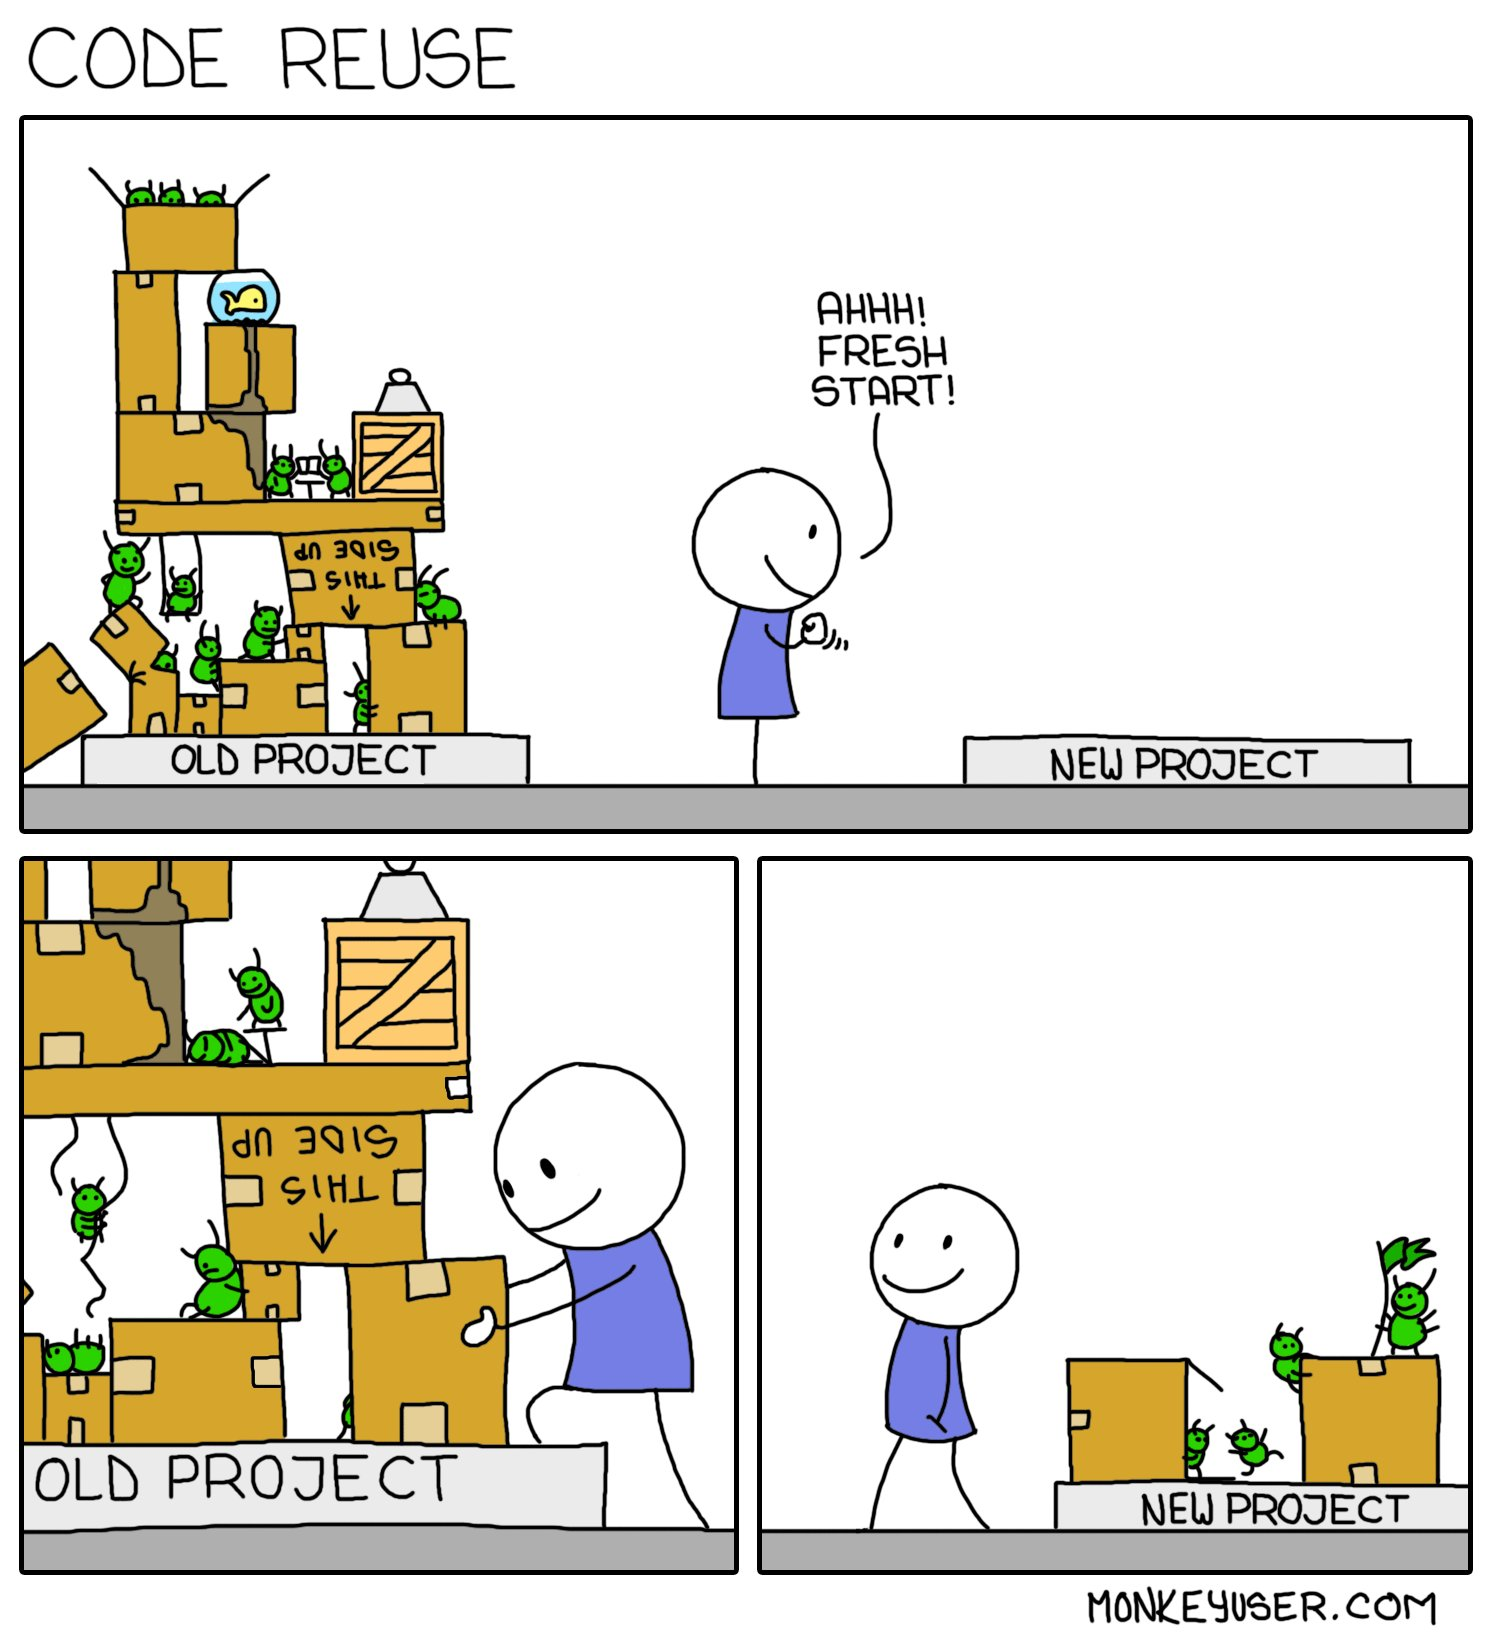
\includegraphics[width=\textwidth,height=2.08333in]{./img/code_reuse.jpg}

\url{https://www.reddit.com/r/ProgrammerHumor/comments/11a1fqi/code_reuse/\#lightbox}

\section{Make R your own}\label{make-r-your-own}

So far, you have learned about many important aspects of getting used to a productive and efficient workflow.
However, in my experience the best basis for a good workflow means nothing if it is not really fun to use said flow.
Therefore, I want to introduce you to a really nifty feature in R Studio: customizing the appearance.

\begin{quote}
\texttt{Tools} \(\rightarrow\) \texttt{Global\ Options} \(\rightarrow\) \texttt{Appearance} 
\includegraphics[width=\textwidth,height=0.3125in]{./img/appearance.png}
\end{quote}

Because honestly? it's fun, and if a program is fun you will want to use it more.
And practice is is the best way of learning any new skill.

There are many different ``themes'' for R Studio to choose from.
You can control not only what the interface looks like but also how code is displayed.
This can be especially helpful if you have a hard time differentiating colors - you can look for a theme that makes it easier for you!
Most themes also have some rules for coloring numbers differently than text differently than function calls an so on.
So it is not just a nice add on but can actually be really helpful and improve accessibility.
Personally, I work really well with the \texttt{Merbivore} theme - what is your favorite?

\section*{Wrap-Up \& Further Resources}\label{wrap-up-further-resources-2}
\addcontentsline{toc}{section}{Wrap-Up \& Further Resources}

Stick to naming conventions for R objects and related files

Make sure your working directory is correct

Use R projects to organize your scripts easily

Make R fun and appealing to use FOR YOU!

\href{https://thedavidchen.github.io/post/rstudio-why-use-projects/}{R Projects: A quick overview}

\href{https://bookdown.org/daniel_dauber_io/r4np_book/starting-your-r-projects.html}{Starting your R projects}

\href{https://martinctc.github.io/blog/rstudio-projects-and-working-directories-a-beginner's-guide/}{RStudio Projects and Directories} (rather thorough)

\href{https://www.tidyverse.org/blog/2017/12/workflow-vs-script/}{Some ideas on improving your workflow} (this can seem a bit advanced, but try reading through anyway and see what sticks with you. Building good habits at the beginning of your learning journey will make your life a lot easier down the line!)

\section*{Working with Version Control}\label{working-with-version-control}
\addcontentsline{toc}{section}{Working with Version Control}

\ldots can sound scary and daunting to learn.
I believe this to be a more advanced feature which is a bit much for a (non-programmer) beginner, so I will mention it last.
However, using version control systems such as \href{https://github.com/}{GitHub} can be really great to keep track of your work, share with others and also ask for help.

If you want to start learning about Git and GitHub, I suggest \href{https://docs.github.com/en/get-started/start-your-journey/about-github-and-git}{starting your journey} directly on the GitHub Docs webpage.
For those who may already have some experience, here is a nice blog article bringing up some of the slips and falls one might take when working with GitHub: \href{https://www.r-bloggers.com/2024/06/hack-your-way-to-a-good-git-history/}{Hack your way to a good Git history (Maëlle Salmon)}.

\chapter*{\texorpdfstring{(PART) Into the \texttt{tidyverse}}{(PART) Into the tidyverse}}\label{part-into-the-tidyverse}

\chapter{\texorpdfstring{Data munging with \texttt{dplyr}}{Data munging with dplyr}}\label{dplyr}

In this chapter you will learn about working with packages, which I find similar to teaching your R new tricks.
I will also introduce you to the \texttt{tidyverse} - a collection of packages and why I strongly suggest to familiarize oneself with a bunch of them.
Spoiler: It will make your life a lot easier.

\section{Working with packages}\label{working-with-packages}

First off, when you stick to the metaphor a package being a collection of tricks to teach your R, then you will teach the tricks once and remind R that it knows the tricks every time you want to use them.
In more real life terms, you will install a package once and load it in each new session.
This is important to remember because installing packages is one of the few things you will \emph{only} want to do in your console - NOT in any of your scripts.
Nothing bad will happen if you do, but it takes a very long time and it will test both your own patience and that of your computer.

Generally, packages can be installed with the \texttt{install.packages()} function.
It needs the package name in quotes as input in the parentheses, e.g.~\texttt{install.packages("dplyr")}.
This means the package is now on your computer but you still need to make it available.
The easiest way to achieve that is to load the whole package using the \texttt{library()} command.
This will usually be done inside a script where you want to use functions from that package.
Later in this chapter, when we look at dplyr functions on the \texttt{iris} data in Section \ref{intro-iris}, you will see a code chunk as a prototype of a typical beginning of an R script.

While \texttt{library()} makes all functions from a package available, you can also only load specific functions right when you want to use them.
This works with the notation \texttt{package::function()} and is particularly useful if (1) the package is extremely large, takes a long time to load and/or you really only need the one function or (b) the function name you want to use is not unique, i.e.~there are several packages that contain a function of that name.
For example, the function \emph{filter} exists in more than one package, so you might use \texttt{dplyr::filter()} in your code to make explicit that you want to use the \texttt{filter()} function from the \texttt{dplyr} package.

When this is the case, you will get the message ``The following objects are masked from\ldots{}'' in the console when you load the package. This is also good to keep in mind if you run into unexpected errors - maybe you meant to use the function from another package but R is using the one you loaded last?

In the interest of creating reproducible code, it can also make sense to use the \texttt{package::function()} notation, so you can explicitly show others which function you used.

At a glance:

\begin{itemize}
\tightlist
\item
  Install packages with \texttt{install.packages()} only once in the console!
\item
  Load packages with \texttt{library()} every time you load a script or start a new session

  \begin{itemize}
  \tightlist
  \item
    Usually in the script, but also in the console
  \end{itemize}
\item
  Specific function from a package: \texttt{package::function()}

  \begin{itemize}
  \tightlist
  \item
    Use if you just need that one function once and don't want load the entire package
  \item
    Or to explicitly show the according package
  \item
    Or the function name is also in other packages (e.g.~``filter'' is usually \texttt{dplyr::filter}, but sometimes \texttt{stats::filter})
  \end{itemize}
\end{itemize}

\section{The tidyverse}\label{the-tidyverse}

\begin{quote}
The tidyverse is an opinionated \textbf{collection of R packages designed for data science}. All packages share an underlying design philosophy, grammar, and data structures. (\url{tidyverse.org})
\end{quote}

So packages are pretty cool: They usually come from people who had a specific problem, found a solution and decided to share it with others so they can more easily fix new problems.
Of course everyone has a different preference on how to work, which is why not every package and function will be intuitive to everyone.
That is also why the definition of an ``opinionated collection of R packages'' is so fitting because the \texttt{tidyverse} is a framework consisting of many different packages that the authors find intuitive and useful.

\begin{figure}
\centering
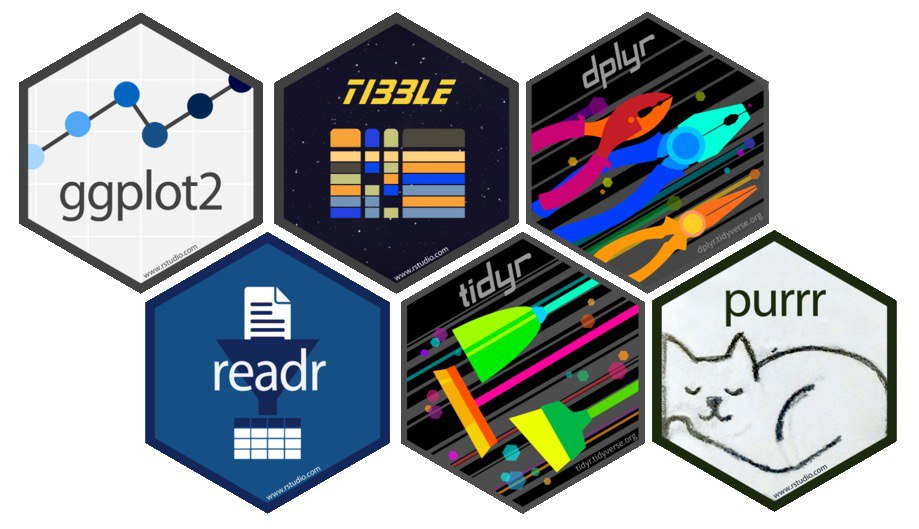
\includegraphics[width=\textwidth,height=2.08333in]{./img/hexagons.png}
\caption{Hex Logos}
\end{figure}

Incidentally, I agree and I will show you why.
If you figure out at some point that your prefer another way - that's great, but the tidyverse is a solid starting point for most data science needs in psychology.

The structure of the \texttt{tidyverse} packages is very clear and they each serve a distinct purpose.
Taking a real-life workflow as inspiration, we will first get to know \texttt{dplyr}, a package for cleaning up data and editing everything to your needs in this chapter and later get to know \texttt{ggplot2} as a package for data visualization in Chapter \ref{ggplot2}.
One of the big advantages of the \texttt{tidyverse} packages is that the can be combined very easily, creating easy-to-read and -write workflows that you will probably still be able to understand one year after you wrote it.\footnote{Being able to read your own code after a while is already challenging but try making sense of code that someone else has written!}

You can install the whole \texttt{tidyverse} at once, which will take a little while as it contains a lot of individual packages.
Generally, I would recommend installing them once, but loading packages individually when you need them, because also loading the bulk of packages takes a lot of time.

\begin{quote}
\texttt{install.packages("tidyverse")}
\end{quote}

\subsection[What is \texttt{dplyr}? ]{\texorpdfstring{What is \texttt{dplyr}? \protect
\includegraphics[width=\textwidth,height=0.83333in]{./img/dplyr.png}}{What is dplyr? dplyr logo}}\label{what-is-dplyr-dplyr-logo}

The \texttt{dplyr} package is probably the best and most important package in R \emph{imho}.
It is a powerful tool for editing data in data frames and a great way to keep your workflow clear and reproducible.
It has very intuitively named functions that on their own already serve most purposes that you will commonly need to properly work with your data.
If you haven't already, now would be a good time to install \texttt{dplyr} and load it into a practice script:

\begin{quote}
\texttt{install.packages("dplyr")} \(\rightarrow\) \texttt{library(dplyr)}
\end{quote}

In the following, we will use a data example to get to know some of the most important functions.
Try to follow along and remember that you can always get more info on a function with a question mark in front of the function name in the console (here best to add the package name), e.g.~\texttt{?dplyr::filter}.
If you want more general information on the whole package you can use the command \texttt{browseVignettes(package\ =\ "dplyr")} in the console.
Also check the \hyperref[wrapupdplyr]{further resources} and an overview of the \hyperref[mif]{most important dplyr functions}.

\section{\texorpdfstring{Intro to \texttt{dplyr}}{Intro to dplyr}}\label{intro-iris}

\begin{figure}
\centering
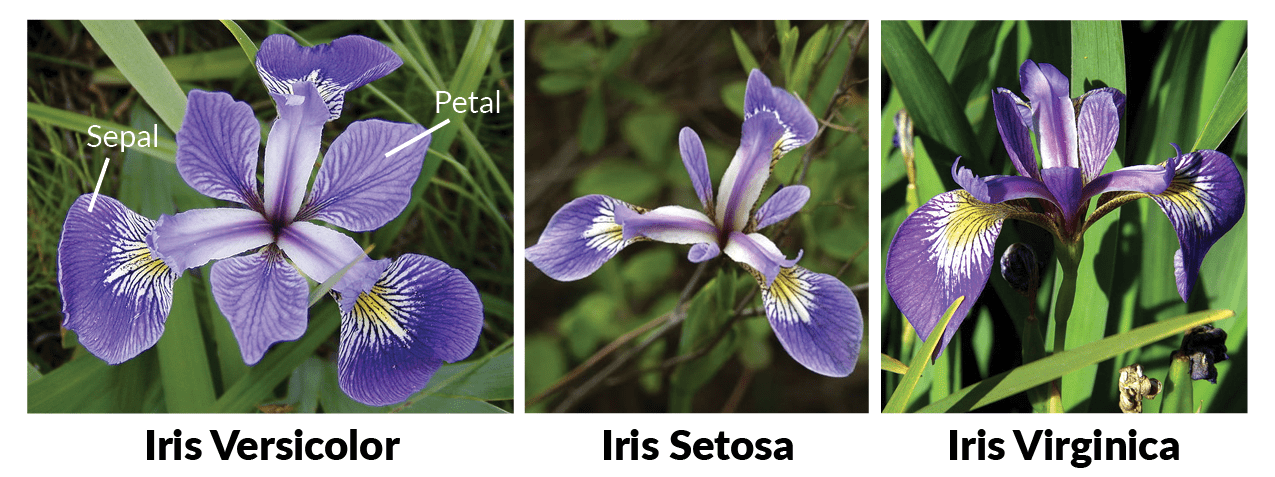
\includegraphics[width=\textwidth,height=1.5625in]{./img/iris-setosa.png}
\caption{Types of Iris Flowers}
\end{figure}

We introduced the \texttt{iris} data set in Section \ref{basics} - a native R data set that you can just access without needing to load anything.
It contains information on iris flowers of different species and we will use the \texttt{glimpse()} function from \texttt{dplyr} to get a first overview of the data we have at hand:

\begin{Shaded}
\begin{Highlighting}[]
\NormalTok{dplyr}\SpecialCharTok{::}\FunctionTok{glimpse}\NormalTok{(iris)}
\CommentTok{\# Rows: 150}
\CommentTok{\# Columns: 5}
\CommentTok{\# $ Sepal.Length \textless{}dbl\textgreater{} 5.1, 4.9, 4.7, 4.6, 5.0, 5.4, 4.6, 5.0, 4.4, 4.9, 5.4, 4.8, 4.8, 4.3, 5.8, 5.7, 5.4, 5.1, 5.7, 5.1, 5.4, 5.1, 4.6, 5.1, \textasciitilde{}}
\CommentTok{\# $ Sepal.Width  \textless{}dbl\textgreater{} 3.5, 3.0, 3.2, 3.1, 3.6, 3.9, 3.4, 3.4, 2.9, 3.1, 3.7, 3.4, 3.0, 3.0, 4.0, 4.4, 3.9, 3.5, 3.8, 3.8, 3.4, 3.7, 3.6, 3.3, \textasciitilde{}}
\CommentTok{\# $ Petal.Length \textless{}dbl\textgreater{} 1.4, 1.4, 1.3, 1.5, 1.4, 1.7, 1.4, 1.5, 1.4, 1.5, 1.5, 1.6, 1.4, 1.1, 1.2, 1.5, 1.3, 1.4, 1.7, 1.5, 1.7, 1.5, 1.0, 1.7, \textasciitilde{}}
\CommentTok{\# $ Petal.Width  \textless{}dbl\textgreater{} 0.2, 0.2, 0.2, 0.2, 0.2, 0.4, 0.3, 0.2, 0.2, 0.1, 0.2, 0.2, 0.1, 0.1, 0.2, 0.4, 0.4, 0.3, 0.3, 0.3, 0.2, 0.4, 0.2, 0.5, \textasciitilde{}}
\CommentTok{\# $ Species      \textless{}fct\textgreater{} setosa, setosa, setosa, setosa, setosa, setosa, setosa, setosa, setosa, setosa, setosa, setosa, setosa, setosa, setosa, \textasciitilde{}}
\end{Highlighting}
\end{Shaded}

\subsection*{Imagine\ldots{}}\label{imagine}
\addcontentsline{toc}{subsection}{Imagine\ldots{}}

When working with ``real'' data, aka survey or experimental data, we will usually need to reshape, filter and generally edit the data a bit.
This may sound a bit sketchy at first, but we do not want to fake or change any data, we just want to ensure that we have the highest-quality data set to work with that we can.

In the example we will be working with, we have the following three goals for the data:

\begin{enumerate}
\def\labelenumi{\arabic{enumi}.}
\tightlist
\item
  We only want data from species ``virginica''.
\item
  We are interested in sepal length.
\item
  We want to adjust variable names.
\item
  We later also want the species to be capitalized in our data \& to add a new binary variable for whether a flower's petals are longer than 5.5 cm (1) or not (0).
\end{enumerate}

Using \texttt{dplyr} functions, we can easily achieve all these goals in a few lines of code.
We will go more into depth

\begin{Shaded}
\begin{Highlighting}[]
\FunctionTok{library}\NormalTok{(dplyr)}

\NormalTok{iris\_virginica }\OtherTok{\textless{}{-}}\NormalTok{ iris }\SpecialCharTok{\%\textgreater{}\%} \CommentTok{\# create new data set as copy}
  \FunctionTok{filter}\NormalTok{(Species }\SpecialCharTok{==} \StringTok{"virginica"}\NormalTok{) }\SpecialCharTok{\%\textgreater{}\%} \CommentTok{\# 1. only virginica}
  \FunctionTok{select}\NormalTok{(Petal.Length, Species)  }\SpecialCharTok{\%\textgreater{}\%} \CommentTok{\# 2. select columns }
  \FunctionTok{rename}\NormalTok{(}\AttributeTok{plength =}\NormalTok{ Petal.Length) }\CommentTok{\# 3. rename variable/column}

\FunctionTok{str}\NormalTok{(iris\_virginica)}
\CommentTok{\# \textquotesingle{}data.frame\textquotesingle{}: 50 obs. of  2 variables:}
\CommentTok{\#  $ plength: num  6 5.1 5.9 5.6 5.8 6.6 4.5 6.3 5.8 6.1 ...}
\CommentTok{\#  $ Species: Factor w/ 3 levels "setosa","versicolor",..: 3 3 3 3 3 3 3 3 3 3 ...}
\end{Highlighting}
\end{Shaded}

\subsection{Filter}\label{filter}

\begin{figure}
\centering
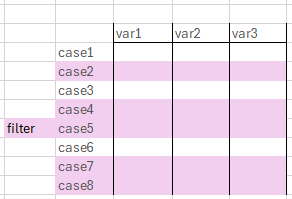
\includegraphics[width=\textwidth,height=1.04167in]{./img/filter.png}
\caption{filter scheme}
\end{figure}

\begin{itemize}
\tightlist
\item
  Filters data by a \textbf{value in a variable}

  \begin{itemize}
  \tightlist
  \item
    With filter we \textbf{keep only certain rows} in our data
  \end{itemize}
\item
  Needs \textbf{logical operators} as input

  \begin{itemize}
  \tightlist
  \item
    ``keep only cases where variable x has value abc''
  \item
    Can also be used with the ! to drop certain cases
  \item
    Drop NAs: \texttt{data\ \%\textgreater{}\%\ filter(!is.na(variable))}
  \end{itemize}
\end{itemize}

\subsection{Select}\label{select}

\begin{figure}
\centering
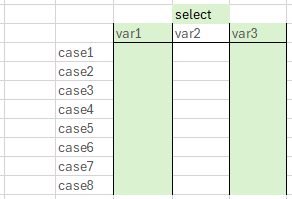
\includegraphics[width=\textwidth,height=1.04167in]{./img/select.png}
\caption{select scheme}
\end{figure}

\begin{itemize}
\tightlist
\item
  Selects \textbf{variables based on their names}

  \begin{itemize}
  \tightlist
  \item
    With select we \textbf{keep only certain columns} in our data
  \end{itemize}
\item
  Needs \textbf{variable names} as input

  \begin{itemize}
  \tightlist
  \item
    ``keep only variables with this name''
  \item
    Can also be used with the ! to drop certain variables
  \end{itemize}
\item
  Cave: if we want to extract one variable to calculate something, you will want to use \texttt{pull()} instead

  \begin{itemize}
  \tightlist
  \item
    Check \texttt{iris\ \%\textgreater{}\%\ select(Species)\ \%\textgreater{}\%\ class()} and \texttt{iris\ \%\textgreater{}\%\ pull(Species)\ \%\textgreater{}\%\ class()}
  \end{itemize}
\end{itemize}

\subsection{Rename}\label{rename}

This is probably the most intuitively named function: It renames a variable in a data frame.
As input the function takes your new variable name, an equal sign and the old variable name.
This order is important, so if you run into an error, make sure that you are using \emph{new\_variable = old\_variable}.
Also, you do not need quotes around your variable names.

\subsection{Mutate}\label{mutate}

\begin{itemize}
\tightlist
\item
  We also want the species to be capitalized in our data
\item
  We also want to add a new binary variable for whether a flower's petals are longer than 5.5 cm (1) or not (0)

  \begin{itemize}
  \tightlist
  \item
    for this, we use the \texttt{ifelse()} function:
  \item
    Needs a logical as first input, then what to do if it's true, last what to do if it's false
  \end{itemize}
\item
  Mutate takes a \textbf{variable name as input} (existing or new) and some \textbf{function or calculation} to be done on that variable
\end{itemize}

\begin{Shaded}
\begin{Highlighting}[]
\NormalTok{iris\_virginica }\OtherTok{\textless{}{-}}\NormalTok{ iris\_virginica }\SpecialCharTok{\%\textgreater{}\%} 
  \FunctionTok{mutate}\NormalTok{(}\AttributeTok{Species =} \FunctionTok{toupper}\NormalTok{(Species), }\CommentTok{\# 4. change content of Species and add new binary variable bigboi}
         \AttributeTok{bigboi =} \FunctionTok{ifelse}\NormalTok{(plength }\SpecialCharTok{\textgreater{}} \FloatTok{5.5}\NormalTok{, }\DecValTok{1}\NormalTok{, }\DecValTok{0}\NormalTok{))}

\FunctionTok{table}\NormalTok{(iris\_virginica}\SpecialCharTok{$}\NormalTok{Species)}
\CommentTok{\# }
\CommentTok{\# VIRGINICA }
\CommentTok{\#        50}
\end{Highlighting}
\end{Shaded}

\subsection{group\_by \& summarize}\label{group_by-summarize}

\begin{itemize}
\tightlist
\item
  With the dplyr-workflow, we can easily output group statistics
\item
  Keywords: \textbf{group\_by()} \& \textbf{summarize()}
\item
  The code is built like any other dplyr workflow with pipes ( \%\textgreater\% ) in between each:

  \begin{enumerate}
  \def\labelenumi{\arabic{enumi}.}
  \tightlist
  \item
    Define/ name the data frame
  \item
    group\_by(\emph{variable\_name})
  \item
    in summarize, define a name for the statistic, use a =, use a function like mean() for the measure
  \end{enumerate}
\end{itemize}

\begin{Shaded}
\begin{Highlighting}[]
\FunctionTok{str}\NormalTok{(Orange) }\CommentTok{\# use different default data set}
\CommentTok{\# Classes \textquotesingle{}nfnGroupedData\textquotesingle{}, \textquotesingle{}nfGroupedData\textquotesingle{}, \textquotesingle{}groupedData\textquotesingle{} and \textquotesingle{}data.frame\textquotesingle{}:    35 obs. of  3 variables:}
\CommentTok{\#  $ Tree         : Ord.factor w/ 5 levels "3"\textless{}"1"\textless{}"5"\textless{}"2"\textless{}..: 2 2 2 2 2 2 2 4 4 4 ...}
\CommentTok{\#  $ age          : num  118 484 664 1004 1231 ...}
\CommentTok{\#  $ circumference: num  30 58 87 115 120 142 145 33 69 111 ...}
\CommentTok{\#  {-} attr(*, "formula")=Class \textquotesingle{}formula\textquotesingle{}  language circumference \textasciitilde{} age | Tree}
\CommentTok{\#   .. ..{-} attr(*, ".Environment")=\textless{}environment: R\_EmptyEnv\textgreater{} }
\CommentTok{\#  {-} attr(*, "labels")=List of 2}
\CommentTok{\#   ..$ x: chr "Time since December 31, 1968"}
\CommentTok{\#   ..$ y: chr "Trunk circumference"}
\CommentTok{\#  {-} attr(*, "units")=List of 2}
\CommentTok{\#   ..$ x: chr "(days)"}
\CommentTok{\#   ..$ y: chr "(mm)"}

\NormalTok{Orange }\SpecialCharTok{\%\textgreater{}\%} 
  \FunctionTok{group\_by}\NormalTok{(Tree) }\SpecialCharTok{\%\textgreater{}\%} 
  \FunctionTok{summarize}\NormalTok{(}\AttributeTok{m\_age =} \FunctionTok{mean}\NormalTok{(age),}
            \AttributeTok{m\_circumference =} \FunctionTok{mean}\NormalTok{(circumference),}
            \AttributeTok{n =} \FunctionTok{n}\NormalTok{())}
\CommentTok{\# \# A tibble: 5 x 4}
\CommentTok{\#   Tree  m\_age m\_circumference     n}
\CommentTok{\#   \textless{}ord\textgreater{} \textless{}dbl\textgreater{}           \textless{}dbl\textgreater{} \textless{}int\textgreater{}}
\CommentTok{\# 1 3      922.            94       7}
\CommentTok{\# 2 1      922.            99.6     7}
\CommentTok{\# 3 5      922.           111.      7}
\CommentTok{\# 4 2      922.           135.      7}
\CommentTok{\# 5 4      922.           139.      7}
\end{Highlighting}
\end{Shaded}

\section*{Exercises}\label{exercises-1}
\addcontentsline{toc}{section}{Exercises}

\subsection*{Data Munging}\label{data-munging}
\addcontentsline{toc}{subsection}{Data Munging}

Imagine we want to edit the iris data set for our colleagues from the US, who are interested in the petal width of the \textbf{setosa} and \textbf{versicolor} species.

\begin{enumerate}
\def\labelenumi{\arabic{enumi}.}
\tightlist
\item
  Create a new dataset from \texttt{iris} with a meaningful name
\item
  \texttt{select()} the variables of interest
\item
  \texttt{filter()} the species that we want

  \begin{itemize}
  \tightlist
  \item
    Use \%in\% to filter by more than one value, or think about a reverse approach\ldots!
  \end{itemize}
\item
  \texttt{rename()} the Petal.Width variable to be named pwidth
\item
  Use \texttt{mutate()} to add a new variable named ``pwidth\_inch'', which contains the petal width in inches

  \begin{itemize}
  \tightlist
  \item
    Calculation: pwidth / 2.54 (2.54 cm = 1 inch)
  \end{itemize}
\end{enumerate}

Solution

\begin{Shaded}
\begin{Highlighting}[]
\NormalTok{iris\_twospec }\OtherTok{\textless{}{-}}\NormalTok{ iris }\SpecialCharTok{\%\textgreater{}\%} 
  \FunctionTok{select}\NormalTok{(Petal.Width, Species) }\SpecialCharTok{\%\textgreater{}\%} 
  \FunctionTok{filter}\NormalTok{(Species }\SpecialCharTok{\%in\%} \FunctionTok{c}\NormalTok{(}\StringTok{"setosa"}\NormalTok{, }\StringTok{"versicolor"}\NormalTok{)) }\SpecialCharTok{\%\textgreater{}\%} 
  \CommentTok{\# or: filter(Species != "virginica")}
  \CommentTok{\# or: filter(Species == c("setosa" | "versicolor"))}
  \FunctionTok{rename}\NormalTok{(}\AttributeTok{pwidth =}\NormalTok{ Petal.Width) }\SpecialCharTok{\%\textgreater{}\%} 
  \FunctionTok{mutate}\NormalTok{(}\AttributeTok{pwidth\_inch =}\NormalTok{ pwidth }\SpecialCharTok{/} \FloatTok{2.54}\NormalTok{)}

\FunctionTok{head}\NormalTok{(iris\_twospec, }\DecValTok{8}\NormalTok{)}
\CommentTok{\#   pwidth Species pwidth\_inch}
\CommentTok{\# 1    0.2  setosa  0.07874016}
\CommentTok{\# 2    0.2  setosa  0.07874016}
\CommentTok{\# 3    0.2  setosa  0.07874016}
\CommentTok{\# 4    0.2  setosa  0.07874016}
\CommentTok{\# 5    0.2  setosa  0.07874016}
\CommentTok{\# 6    0.4  setosa  0.15748031}
\CommentTok{\# 7    0.3  setosa  0.11811024}
\CommentTok{\# 8    0.2  setosa  0.07874016}
\end{Highlighting}
\end{Shaded}

\begin{figure}
\centering

\includegraphics[width=\textwidth,height=2.08333in]{./img/hadley-meme.png}
\caption{Hadley Wickham, developer of the tidyverse}
\end{figure}

\subsection*{Group Statistics}\label{group-statistics}
\addcontentsline{toc}{subsection}{Group Statistics}

Follow the structure to group the iris data set by Species and output a summary with the mean values of all four other variables in the data.
Also include the grouped n.

Solution

\begin{Shaded}
\begin{Highlighting}[]
\NormalTok{iris }\SpecialCharTok{\%\textgreater{}\%} 
  \FunctionTok{group\_by}\NormalTok{(Species) }\SpecialCharTok{\%\textgreater{}\%} 
  \FunctionTok{summarize}\NormalTok{(}\AttributeTok{m\_plength =} \FunctionTok{mean}\NormalTok{(Petal.Length),}
            \AttributeTok{m\_pwidth =} \FunctionTok{mean}\NormalTok{(Petal.Width),}
            \AttributeTok{m\_slength =} \FunctionTok{mean}\NormalTok{(Sepal.Length),}
            \AttributeTok{m\_swidth =} \FunctionTok{mean}\NormalTok{(Sepal.Width),}
            \AttributeTok{n =} \FunctionTok{n}\NormalTok{())}
\CommentTok{\# \# A tibble: 3 x 6}
\CommentTok{\#   Species    m\_plength m\_pwidth m\_slength m\_swidth     n}
\CommentTok{\#   \textless{}fct\textgreater{}          \textless{}dbl\textgreater{}    \textless{}dbl\textgreater{}     \textless{}dbl\textgreater{}    \textless{}dbl\textgreater{} \textless{}int\textgreater{}}
\CommentTok{\# 1 setosa          1.46    0.246      5.01     3.43    50}
\CommentTok{\# 2 versicolor      4.26    1.33       5.94     2.77    50}
\CommentTok{\# 3 virginica       5.55    2.03       6.59     2.97    50}
\end{Highlighting}
\end{Shaded}

\section*{Piping Hot \%\textgreater\%}\label{piping-hot}
\addcontentsline{toc}{section}{Piping Hot \%\textgreater\%}

You already heard about the pipe operator in Section @ref(\#pipe1).
The pipe - available as a native R pipe \textbar\textgreater{} or a \texttt{tidyverse} pipe from the \texttt{magrittr} package \%\textgreater\%\footnote{The two pipes can pretty much the same operations - for specific differences see \url{https://www.tidyverse.org/blog/2023/04/base-vs-magrittr-pipe/}} - takes the input from the left-hand to the right-hand.
In simpler terms, it takes the operation you did before the pipe and uses is as input for the function after the pipe.
This keeps our code readable and tidy and allows us to keep edits in separate lines, but we still only have to run one command for every task we need
It's easy to add new commands by using another pipe operator, or to leave edits out but commenting out the respective line of code.

It is important to say that most things can be achieved with or without pipe and you may prefer different versions for different tasks.
You have seen a basic example of the use of the pipe operator in Section @ref(\#pipe1), so now we will look at a more sophisticated example: We will perform similar operations as we did above and code them first with pipe and then without.

\begin{Shaded}
\begin{Highlighting}[]
\CommentTok{\# With pipe}
\NormalTok{iris\_edit }\OtherTok{\textless{}{-}}\NormalTok{ iris }\SpecialCharTok{\%\textgreater{}\%}
 \FunctionTok{filter}\NormalTok{(Petal.Length }\SpecialCharTok{\textgreater{}} \DecValTok{3}\NormalTok{) }\SpecialCharTok{\%\textgreater{}\%} \CommentTok{\# only big petals}
 \FunctionTok{select}\NormalTok{(Species, Petal.Length, Sepal.Length) }\SpecialCharTok{\%\textgreater{}\%}  \CommentTok{\# only those columns}
 \FunctionTok{mutate}\NormalTok{(}\AttributeTok{random\_calculation =}\NormalTok{ Petal.Length }\SpecialCharTok{*}\NormalTok{ Sepal.Length) }\CommentTok{\# calculate random new variable}

\CommentTok{\# Without pipe {-} two versions }
\NormalTok{iris\_edit2 }\OtherTok{\textless{}{-}} \FunctionTok{filter}\NormalTok{(iris, Petal.Length }\SpecialCharTok{\textgreater{}} \DecValTok{3}\NormalTok{)}
\NormalTok{iris\_edit2 }\OtherTok{\textless{}{-}} \FunctionTok{select}\NormalTok{(iris\_edit2, Species, Petal.Length, Sepal.Length)}
\NormalTok{iris\_edit2 }\OtherTok{\textless{}{-}} \FunctionTok{mutate}\NormalTok{(iris\_edit2, }\AttributeTok{random\_calculation =}\NormalTok{ Petal.Length }\SpecialCharTok{*}\NormalTok{ Sepal.Length)}

\NormalTok{iris\_edit3 }\OtherTok{\textless{}{-}} \FunctionTok{mutate}\NormalTok{(}
  \FunctionTok{select}\NormalTok{(}
    \FunctionTok{filter}\NormalTok{(}
\NormalTok{      iris, Petal.Length }\SpecialCharTok{\textgreater{}} \DecValTok{3}
\NormalTok{    ),}
\NormalTok{    Species, Petal.Length, Sepal.Length}
\NormalTok{  ), }
  \AttributeTok{random\_calculation =}\NormalTok{ Petal.Length }\SpecialCharTok{*}\NormalTok{ Sepal.Length}
\NormalTok{)}

\CommentTok{\# Are the three versions equal?}
\FunctionTok{all.equal}\NormalTok{(iris\_edit, iris\_edit2) }\SpecialCharTok{\&} \FunctionTok{all.equal}\NormalTok{(iris\_edit, iris\_edit3)}
\CommentTok{\# [1] TRUE}
\end{Highlighting}
\end{Shaded}

As you can see, all three version produce the same output and all are technically correct.
However, in the second example we keep re-assigning new edits to the same data frame (would be even more annoying but possible to assign each edit to a new data frame) and the third version is just quite the nightmare to read if you ask me.
Also think about this:

\begin{quote}
In the part with pipe we used the \texttt{iris} data to edit and assigned it to \texttt{iris\_edit}.
In version two without pipe we used \texttt{iris} in the first line, but afterwards we used \texttt{iris\_edit2} for assignments and edits.
Why is that?
\end{quote}

If we were to use \texttt{iris} in each line, it would overwrite the last edit every time.

We can also profit from the pipe in base-R or with a larger combination of different functions.
Usually, the pipe helps us not to drown in parentheses when conducting analyses.
Let's e.g.~calculate a mean value after filtering by Species setosa.

So without a pipe, it might look like this:

\begin{Shaded}
\begin{Highlighting}[]
\FunctionTok{round}\NormalTok{(}\FunctionTok{mean}\NormalTok{(iris}\SpecialCharTok{$}\NormalTok{Petal.Length[iris}\SpecialCharTok{$}\NormalTok{Species }\SpecialCharTok{==} \StringTok{"setosa"}\NormalTok{]), }\AttributeTok{digits =} \DecValTok{2}\NormalTok{)}
\CommentTok{\# [1] 1.46}
\end{Highlighting}
\end{Shaded}

Using all pipes, the code would look a lot longer but still easier to read.

\begin{Shaded}
\begin{Highlighting}[]
\NormalTok{iris }\SpecialCharTok{\%\textgreater{}\%} 
\FunctionTok{filter}\NormalTok{(Species }\SpecialCharTok{==} \StringTok{"setosa"}\NormalTok{) }\SpecialCharTok{\%\textgreater{}\%} 
\FunctionTok{pull}\NormalTok{(Petal.Length) }\SpecialCharTok{\%\textgreater{}\%}
\FunctionTok{mean}\NormalTok{() }\SpecialCharTok{\%\textgreater{}\%} \FunctionTok{round}\NormalTok{(}\AttributeTok{digits =} \DecValTok{2}\NormalTok{)}
\CommentTok{\# [1] 1.46}
\end{Highlighting}
\end{Shaded}

As a third alternative, we might also use a combination of the approaches, such as:

\begin{Shaded}
\begin{Highlighting}[]
\FunctionTok{round}\NormalTok{(}\FunctionTok{mean}\NormalTok{(}\FunctionTok{filter}\NormalTok{(iris, Species }\SpecialCharTok{==} \StringTok{"setosa"}\NormalTok{) }\SpecialCharTok{\%\textgreater{}\%} \FunctionTok{pull}\NormalTok{(Petal.Length)), }\AttributeTok{digits =} \DecValTok{2}\NormalTok{)}
\CommentTok{\# [1] 1.46}
\end{Highlighting}
\end{Shaded}

As with most things in R and programming, different approaches may be easier in different situations, so it has merit to think outside the box at times!

\begin{quote}
Brainteaser :
We want to edit the iris data to rename a Petal.Length to pl and mutate it to be multiplied by ten.
Why does the first version work, but not the second one?
\end{quote}

\begin{Shaded}
\begin{Highlighting}[]
\CommentTok{\# Version 1}
\NormalTok{iris }\SpecialCharTok{\%\textgreater{}\%} 
  \FunctionTok{mutate}\NormalTok{(}\AttributeTok{Petal.Length =}\NormalTok{ Petal.Length }\SpecialCharTok{*} \DecValTok{10}\NormalTok{) }\SpecialCharTok{\%\textgreater{}\%} 
  \FunctionTok{rename}\NormalTok{(}\AttributeTok{pl =}\NormalTok{ Petal.Length) }\SpecialCharTok{\%\textgreater{}\%} 
  \FunctionTok{glimpse}\NormalTok{()}

\CommentTok{\# Version 2}
\NormalTok{iris }\SpecialCharTok{\%\textgreater{}\%} 
  \FunctionTok{rename}\NormalTok{(}\AttributeTok{pl =}\NormalTok{ Petal.Length) }\SpecialCharTok{\%\textgreater{}\%} 
  \FunctionTok{mutate}\NormalTok{(}\AttributeTok{Petal.Length =}\NormalTok{ Petal.Length }\SpecialCharTok{*} \DecValTok{10}\NormalTok{) }\SpecialCharTok{\%\textgreater{}\%} 
  \FunctionTok{glimpse}\NormalTok{()}
\end{Highlighting}
\end{Shaded}

In the second version, we rename the variable Petal.Length to pl and afterwards try to access it with its old name.

\section*{Wrap-Up \& Further Resources}\label{wrapupdplyr}
\addcontentsline{toc}{section}{Wrap-Up \& Further Resources}

Packages make working with R easier

\texttt{dplyr} is a powerful tool for editing data (\emph{select, filter, mutate\ldots{}})

The pipe \%\textgreater\% makes your code clearer and ``follows the thought process''

\href{https://r4ds.hadley.nz/}{R for Data Science} Book

\href{https://dplyr.tidyverse.org/}{dplyr vignette}

\href{https://r4ds.hadley.nz/data-transform.html\#sec-the-pipe}{Pipe operator}

Cheatsheet: \url{https://github.com/rstudio/cheatsheets/blob/main/data-transformation.pdf}

\href{https://www.youtube.com/watch?v=npOf6aXdguY&ab_channel=RichardOnData}{YouTube: 20 R Packages that you should know} - you for sure don't need them all, but there are some nice inspirations for working with packages in there

\begin{figure}
\centering

\includegraphics[width=\textwidth,height=4.16667in]{./img/idiotic.png}
\caption{Which idiot\ldots{}}\label{id}
\end{figure}

\chapter{\texorpdfstring{Pretty plots with \texttt{ggplot2}}{Pretty plots with ggplot2}}\label{ggplot2}

As you may have gathered by now, I strongly believe that learning (R) should be fun in order to motivate people to keep going.
I also strongly believe that being able to literally look at your data is immensely helpful in understanding the type of statistics you can calculate with it, what the distribution looks like and what generally we are dealing with.
Therefore, we will learn how to make our data visible to both us and others and get to know \texttt{ggplot2} as powerful data visualization package from the \texttt{tidyverse}

\section{\texorpdfstring{Data Visalization }{Data Visalization }}\label{data-visalization}

Data Visualization or data viz for short is an important part of reporting any data in any context.
Drawing a pirate map where X marks the spot could be data visualization as well as a professional statistic of political vote tallies in bar plots.
In general, humans are very visual creatures, so readers/ listeners can follow along more when there is something to look at that illustrates the point.

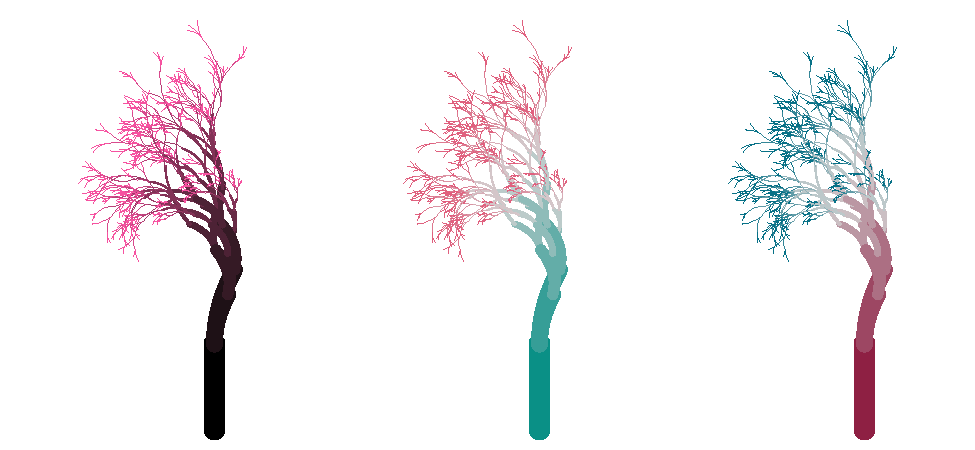
\includegraphics{_main_files/figure-html/flametrees-1.pdf}

The type of visualization to choose strongly depends on what we want to accomplish, who the audience is and of course on the general setting.
While the so-called \emph{flametrees} above are nice to look at, the don't tell us too much about any data as-is.
With reporting statistics, however, we want to be able to \emph{see} our data ¯\textbackslash\_(ツ)\_/¯.
Having a visual representation can be helpful in understanding relationships between variables which helps us and consumers to interpret the results of analyses more intuitively.
Moreover, many common statistics make assumptions about the \emph{distribution} of our data, so we need to check and test that!

\subsection{Example: Sine \& Cosine}\label{example-sine-cosine}

An illustrative example of why it can be very helpful to \emph{see} data before making assumptions is the relationship between sine and cosine.
We won't get too mathematical, but just know they are trigonometric angle functions with a special relationship.
Commonly in psychology, relation = correlation, which assumes a linear relationship.
However, when we take a look at both the correlation between sine and cosine as well as their relationship represented visually, we might see a problem:

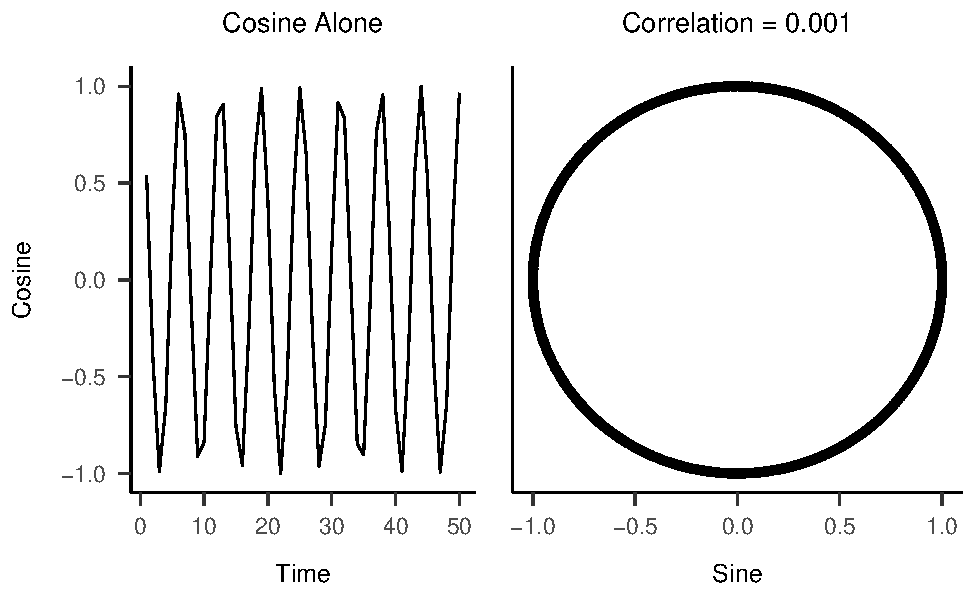
\includegraphics{_main_files/figure-html/unnamed-chunk-30-1.pdf}

We can see that the two variables clearly have a certain type of relation with each other which is definitely not linear.
But if we only reported the very very small correlation of .001, one could assume they had no relation at all!
Keeping that in mind, let's see how we can create beautiful and concise visualizations in R!

\section{\texorpdfstring{What is \texttt{ggplot2}?}{What is ggplot2?}}\label{what-is-ggplot2}

First off, it is probably the best data visualization package in R.
Like \texttt{dplyr} it is part of the \texttt{tidyverse}, so you can expect fairly intuitively named functions and a clear structure that you can build up as you go. ♥
If you have not yet installed the whole \texttt{tidyverse}, you can install \texttt{ggplot2} individually with \texttt{install.packages("ggplot2")}.
Once installed, you can load it with \texttt{library(ggplot2)}.

With \texttt{ggplot2} you can build your plots layer by layer.
Here you can see a schematic of the different elements that can be added to any plot:


\includegraphics{./img/ggplot2layers.png}

\url{https://ggplot2.tidyverse.org/articles/ggplot2.html}

There are two main functions, or rather types of function in this package.

\subsection*{\texorpdfstring{\texttt{ggplot()}}{ggplot()}}\label{ggplot}
\addcontentsline{toc}{subsection}{\texttt{ggplot()}}

This is the main function for ``opening the canvas'', so it basically prepares R for the plot definition.
Commonly, we define the data set (the \emph{Data} layer of the schematic) and which variables to plot in this function (the \emph{Mapping} layer).
The mapping needs the \emph{aesthetics} function \texttt{aes()} as input, in which the variable(s) to be plotted will be defined.

\begin{quote}
It's important to remember that the package is
called \emph{ggplot\textbf{2}} while the function call is \emph{ggplot}!
\end{quote}

\subsection*{\texorpdfstring{\texttt{geom\_XYZ()}}{geom\_XYZ()}}\label{geom_xyz}
\addcontentsline{toc}{subsection}{\texttt{geom\_XYZ()}}

\begin{itemize}
\tightlist
\item
  Defines the actual type of plot = \emph{geometric objects}
\item
  When data is pre-defined, this function does not \emph{need} additional input
\item
  Can handle some ``pretty makers'', such as \texttt{alpha}, which defines color opacity
\item
  \emph{geom\_bar, geom\_boxplot, geom\_density, geom\_jitter, geom\_histogram}
\end{itemize}

\section{Your First Bar Plot}\label{your-first-bar-plot}

\begin{Shaded}
\begin{Highlighting}[]
\FunctionTok{ggplot}\NormalTok{(iris) }\SpecialCharTok{+} 
  \FunctionTok{geom\_bar}\NormalTok{(}\FunctionTok{aes}\NormalTok{(}\AttributeTok{x =}\NormalTok{ Petal.Width)) }
\end{Highlighting}
\end{Shaded}

\begin{flushleft}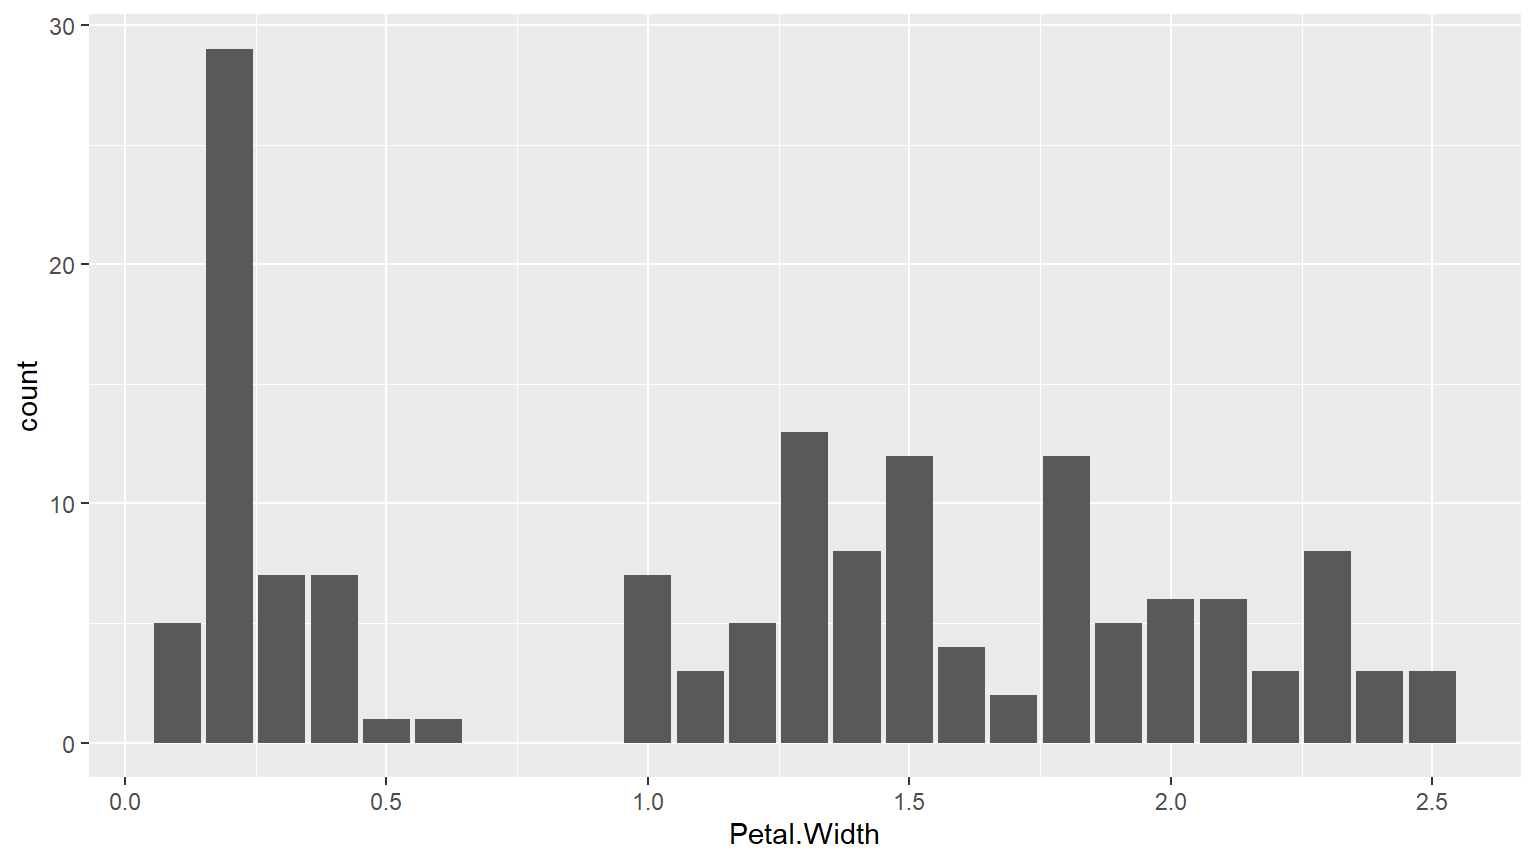
\includegraphics{_main_files/figure-html/unnamed-chunk-31-1} \end{flushleft}

\subsection{Making Plots Prettier}\label{making-plots-prettier}

\begin{itemize}
\tightlist
\item
  color

  \begin{itemize}
  \tightlist
  \item
    visual property of the geometric object
  \item
    which color for the outlines
  \item
    \texttt{colors()}
  \end{itemize}
\item
  fill

  \begin{itemize}
  \tightlist
  \item
    visual property of the geometric object
  \item
    which color to fill
  \end{itemize}
\item
  labs
\item
  theme

  \begin{itemize}
  \tightlist
  \item
    \texttt{install.packages("papaja")} \(\rightarrow\) \texttt{library(papaja)}
  \end{itemize}
\end{itemize}

\subsection{Example: Bar Plot with color and fill}\label{example-bar-plot-with-color-and-fill}

\begin{Shaded}
\begin{Highlighting}[]
\FunctionTok{ggplot}\NormalTok{(iris) }\SpecialCharTok{+} 
  \FunctionTok{geom\_bar}\NormalTok{(}\FunctionTok{aes}\NormalTok{(}\AttributeTok{x =}\NormalTok{ Petal.Width), }\AttributeTok{color =} \StringTok{"deepskyblue3"}\NormalTok{, }\AttributeTok{fill =} \StringTok{"deepskyblue"}\NormalTok{)}
\end{Highlighting}
\end{Shaded}

\begin{flushleft}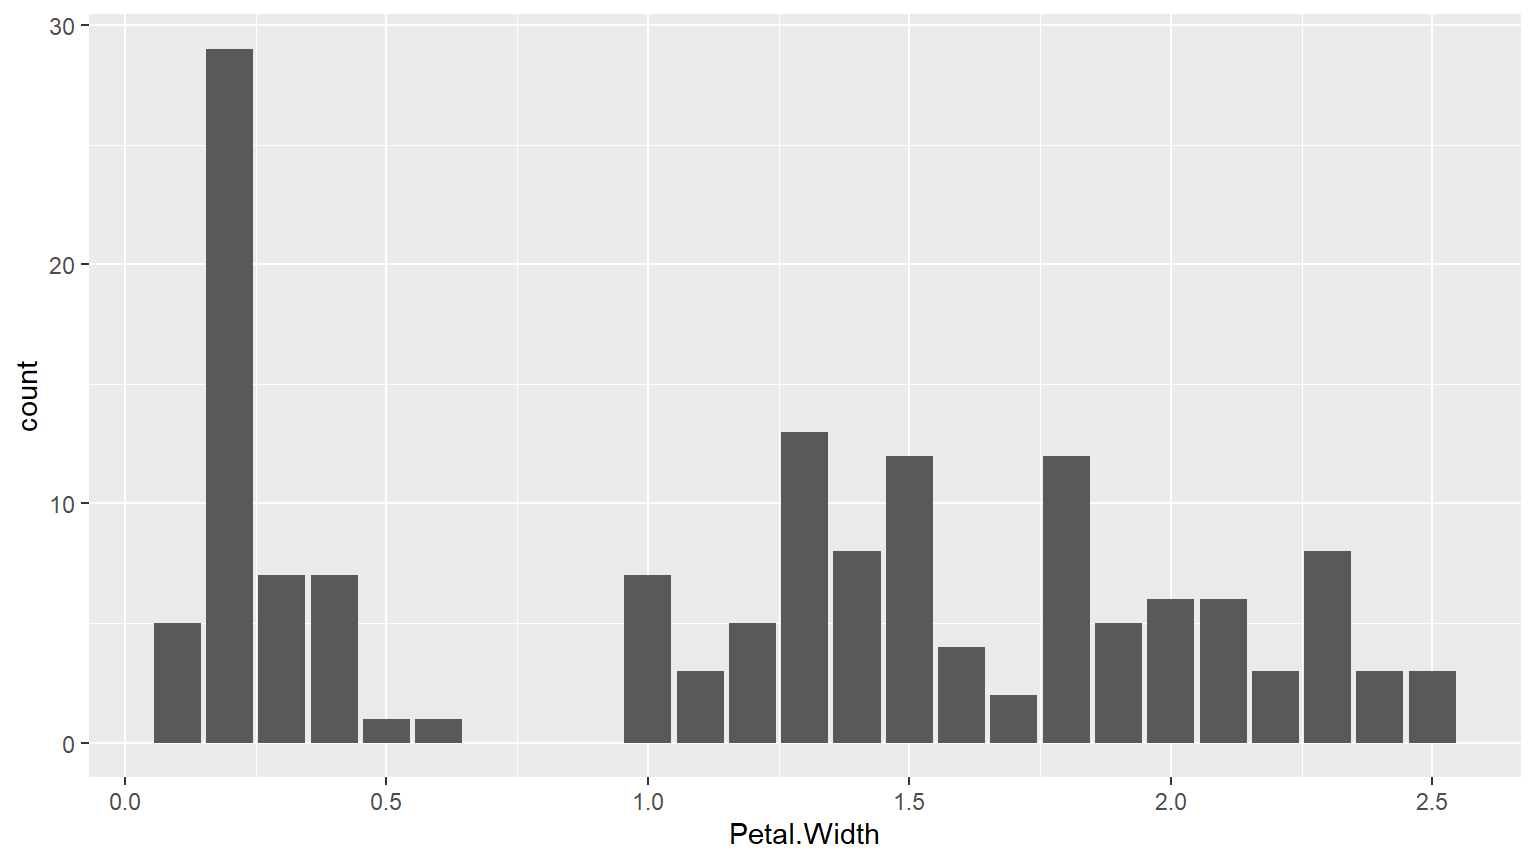
\includegraphics{_main_files/figure-html/unnamed-chunk-32-1} \end{flushleft}

\begin{quote}
What could cause this distribution?
\end{quote}

\begin{Shaded}
\begin{Highlighting}[]
\FunctionTok{ggplot}\NormalTok{(iris) }\SpecialCharTok{+} 
  \FunctionTok{geom\_bar}\NormalTok{(}\FunctionTok{aes}\NormalTok{(}\AttributeTok{x =}\NormalTok{ Petal.Width, }\AttributeTok{color =}\NormalTok{ Species, }\AttributeTok{fill =}\NormalTok{ Species))}
\end{Highlighting}
\end{Shaded}

\begin{flushleft}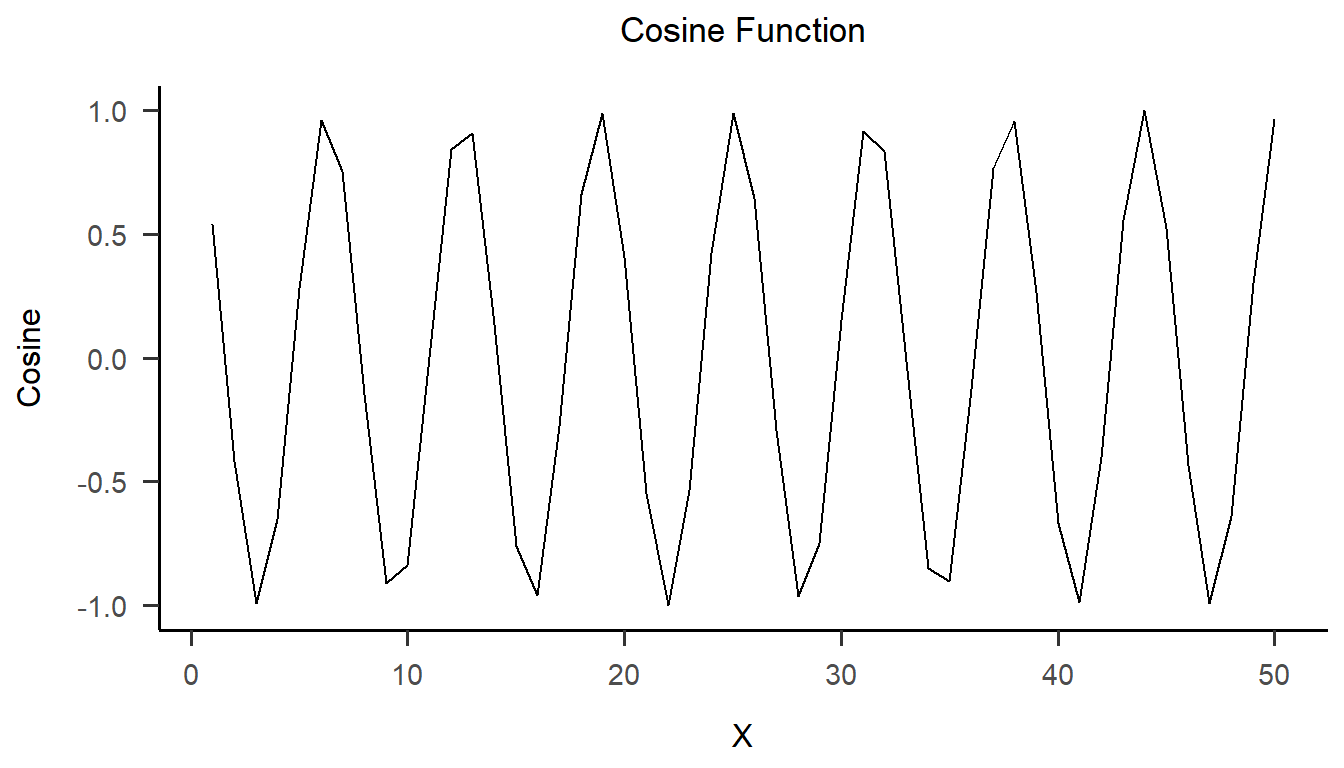
\includegraphics{_main_files/figure-html/unnamed-chunk-33-1} \end{flushleft}

\begin{quote}
What do you notice about the code compared to before?
\end{quote}

\section{Static vs.~Dynamic Aesthetics}\label{static-vs.-dynamic-aesthetics}

\begin{itemize}
\tightlist
\item
  \textbf{Static Aesthetics}: Fixed values applied to all elements of the plot

  \begin{itemize}
  \tightlist
  \item
    Example: \emph{color = ``deepskyblue3''}
  \item
    Means every element will have the same color.
  \end{itemize}
\item
  \textbf{Dynamic Aesthetics}: These map a variable in your data to an aesthetic, which allows different elements to have different colors based on the data

  \begin{itemize}
  \tightlist
  \item
    Example: \emph{aes(color = Species)}
  \item
    Means the color will vary according to the Species variable in the data set.
  \end{itemize}
\end{itemize}

\subsection{Exercise}\label{exercise-1}

Create a \textbf{density plot} that shows \emph{Sepal.Length} from the \texttt{iris} data set.
\emph{Fill} in the color depending on the Species and \emph{color} the outlines with ``white''.
Make sure everything is visible and legible, so try to use an \emph{alpha} of around 0.6.

\begin{Shaded}
\begin{Highlighting}[]
\FunctionTok{ggplot}\NormalTok{(data) }\SpecialCharTok{+} 
  \FunctionTok{geom\_XYZ}\NormalTok{(}\FunctionTok{aes}\NormalTok{(), }\AttributeTok{alpha =}\NormalTok{ ?)}
\end{Highlighting}
\end{Shaded}

\subsection{Solution}\label{solution}

\begin{Shaded}
\begin{Highlighting}[]
\FunctionTok{ggplot}\NormalTok{(iris) }\SpecialCharTok{+} 
  \FunctionTok{geom\_density}\NormalTok{(}\FunctionTok{aes}\NormalTok{(}\AttributeTok{x =}\NormalTok{ Sepal.Length, }\AttributeTok{fill =}\NormalTok{ Species), }
               \AttributeTok{color =} \StringTok{"white"}\NormalTok{, }\AttributeTok{alpha =}\NormalTok{ .}\DecValTok{6}\NormalTok{)}
\end{Highlighting}
\end{Shaded}

\begin{flushleft}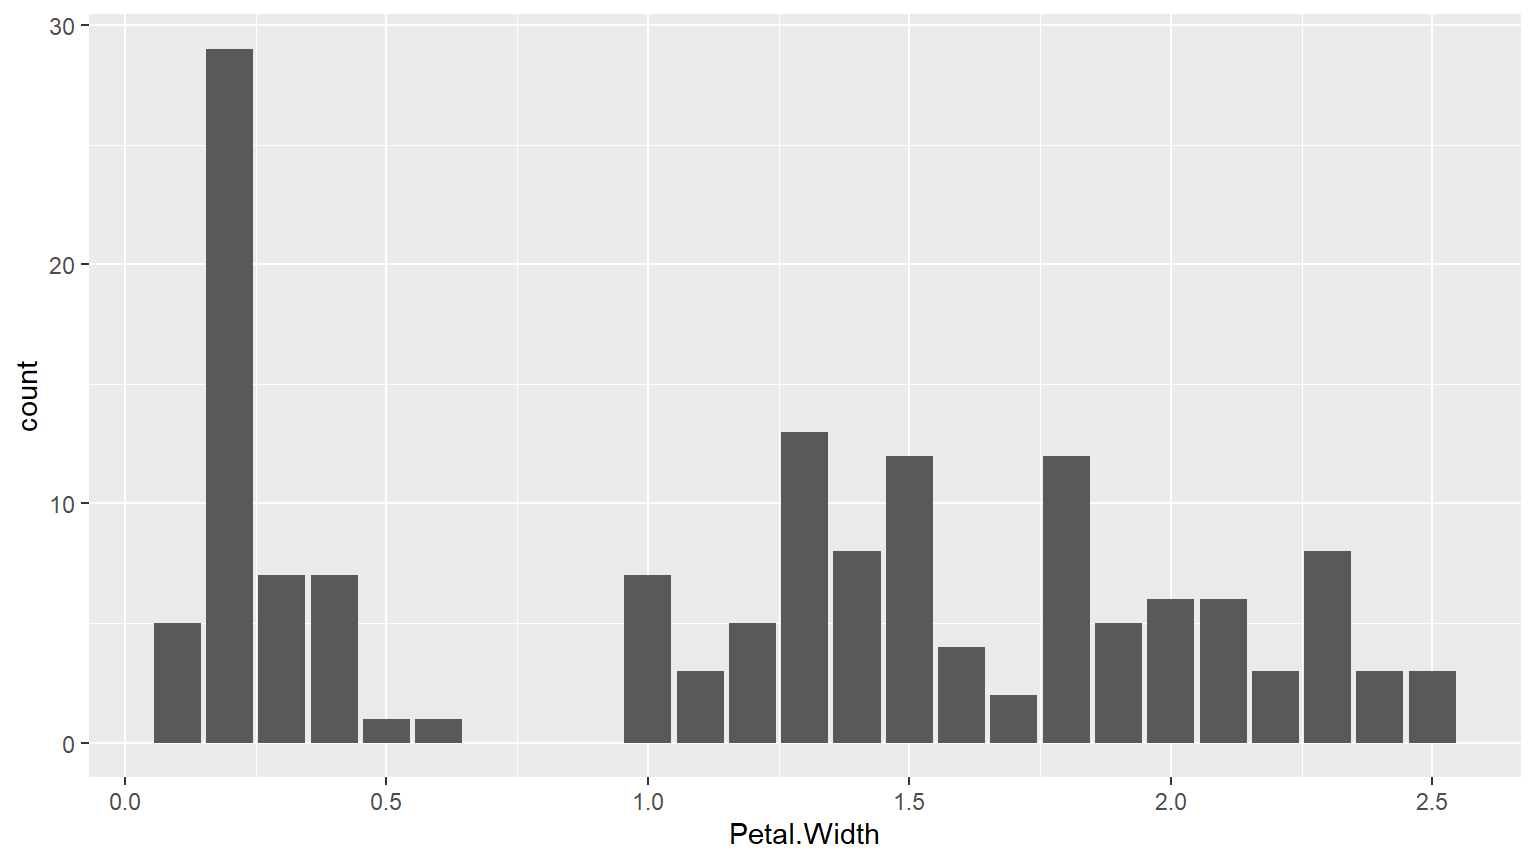
\includegraphics{_main_files/figure-html/unnamed-chunk-35-1} \end{flushleft}

\section{Adding labels and themes}\label{adding-labels-and-themes}

\begin{itemize}
\tightlist
\item
  A good plot should be self explanatory and clear
\item
  We need labels to tell others what our plot shows

  \begin{itemize}
  \tightlist
  \item
    Especially when using color for another variable, it needs to be clear what each color means
  \end{itemize}
\item
  Also the gray-ish default background is ok, but neither very pretty nor very clear

  \begin{itemize}
  \tightlist
  \item
    It is sometimes advisable to keep grid lines visible, but sometimes they can be distracting and unnecessary
  \item
    ggplot2 has a lot of built-in theme options, but there are many packages that provide their own themes
  \item
    Usually \emph{my preference} is \texttt{papaja::theme\_apa()}, which adheres to APA guidelines
  \end{itemize}
\end{itemize}

\begin{Shaded}
\begin{Highlighting}[]
\FunctionTok{ggplot}\NormalTok{(iris) }\SpecialCharTok{+} 
  \FunctionTok{geom\_bar}\NormalTok{(}\FunctionTok{aes}\NormalTok{(}\AttributeTok{x =}\NormalTok{ Petal.Width, }\AttributeTok{color =}\NormalTok{ Species, }\AttributeTok{fill =}\NormalTok{ Species)) }\SpecialCharTok{+}
  \FunctionTok{theme\_apa}\NormalTok{() }\SpecialCharTok{+}
  \FunctionTok{labs}\NormalTok{(}\AttributeTok{x =} \StringTok{"Petal Width"}\NormalTok{, }\AttributeTok{y =} \StringTok{"Flower Count"}\NormalTok{,}
       \AttributeTok{title =} \StringTok{"Size of Iris Flowers"}\NormalTok{)}
\end{Highlighting}
\end{Shaded}

\begin{flushleft}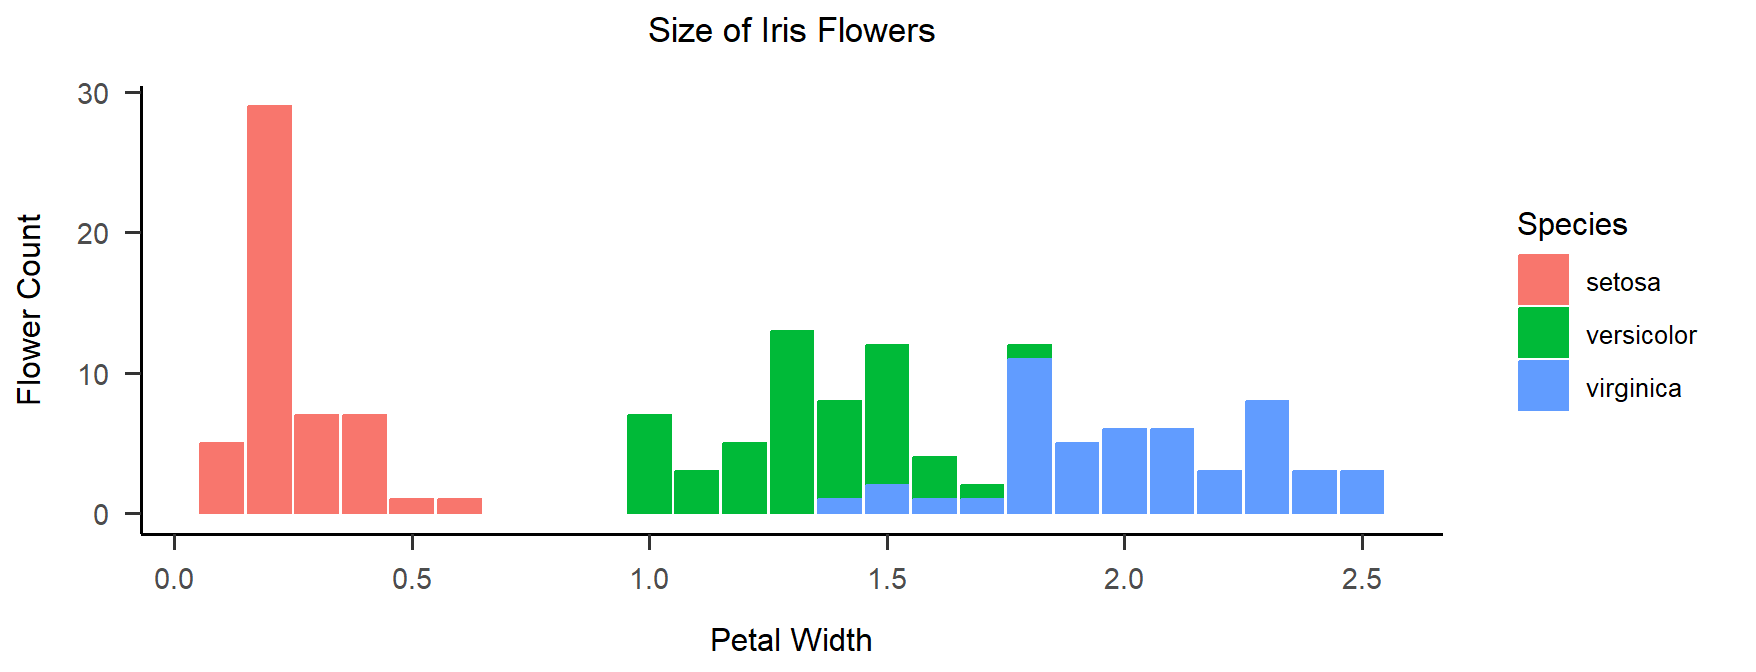
\includegraphics{_main_files/figure-html/themeslabels-1} \end{flushleft}

\section{Bivariate Visualizations}\label{bivariate-visualizations}

\begin{itemize}
\tightlist
\item
  The bar plot shows the distribution of a single variable

  \begin{itemize}
  \tightlist
  \item
    We can add color to show groups
  \end{itemize}
\item
  Showing the relationship of two variables to each other is crucial for understanding our data

  \begin{itemize}
  \tightlist
  \item
    We can still add color to make existing groups clearer or add a third variable
  \end{itemize}
\item
  For a broad overview of which visualization (and statistic) to use for which type of data, visit the \href{https://the-tave.shinyapps.io/Statistics-Picker/}{Statistics Picker} (currently only available in German)

  \begin{itemize}
  \tightlist
  \item
    Most common are boxplots, scatterplots \& line graphs
  \end{itemize}
\end{itemize}

\subsection{Boxplot Example}\label{boxplot-example}

As suggested by one of you, we will look at the relationship of preferred music genre and music volume in our course:

\begin{Shaded}
\begin{Highlighting}[]
\CommentTok{\# seminar \textless{}{-} readRDS("./data/seminar\_data.Rds")}
\FunctionTok{ggplot}\NormalTok{(seminar, }\FunctionTok{aes}\NormalTok{(}\AttributeTok{x=}\NormalTok{v07\_genre, }\AttributeTok{y=}\NormalTok{v08\_loudness, }\AttributeTok{colour=}\NormalTok{v07\_genre, }\AttributeTok{fill=}\NormalTok{v07\_genre)) }\SpecialCharTok{+}
  \FunctionTok{geom\_boxplot}\NormalTok{(}\AttributeTok{alpha =} \FloatTok{0.7}\NormalTok{) }\SpecialCharTok{+} \FunctionTok{theme\_apa}\NormalTok{() }\SpecialCharTok{+}
  \FunctionTok{labs}\NormalTok{(}\AttributeTok{x =} \StringTok{"Preferred Music Genre"}\NormalTok{, }\AttributeTok{y =} \StringTok{"Loudness (arbitrary units)"}\NormalTok{, }
       \AttributeTok{color =} \StringTok{"Genre"}\NormalTok{, }\AttributeTok{fill =} \StringTok{"Genre"}\NormalTok{)}
\end{Highlighting}
\end{Shaded}

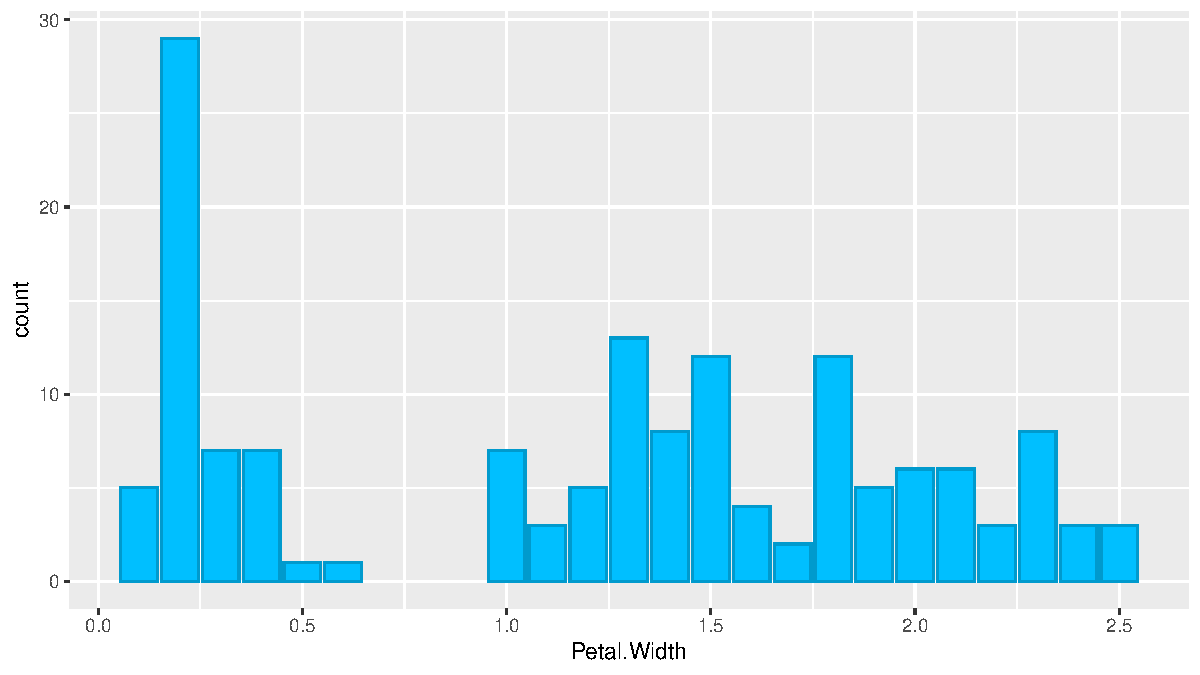
\includegraphics{_main_files/figure-html/unnamed-chunk-36-1.pdf}

\subsection{Exercise: Boxplot}\label{exercise-boxplot}

Create a \textbf{box plot} that shows \emph{Sepal.Length} from the \texttt{iris} data set grouped by the \emph{Species}.
\emph{Fill} and \emph{color} depending on the Species.
Make sure everything is visible and legible, so try to use an \emph{alpha} of around 0.7.
Try to add \emph{labels} and a \emph{theme}.

Solution

\begin{Shaded}
\begin{Highlighting}[]
\FunctionTok{ggplot}\NormalTok{(iris) }\SpecialCharTok{+} 
  \FunctionTok{geom\_boxplot}\NormalTok{(}\FunctionTok{aes}\NormalTok{(}\AttributeTok{x =}\NormalTok{ Species, }\AttributeTok{y =}\NormalTok{ Sepal.Length,}
                   \AttributeTok{color =}\NormalTok{ Species, }\AttributeTok{fill =}\NormalTok{ Species), }\AttributeTok{alpha =}\NormalTok{ .}\DecValTok{6}\NormalTok{) }\SpecialCharTok{+}
  \FunctionTok{theme\_minimal}\NormalTok{() }\SpecialCharTok{+} \FunctionTok{labs}\NormalTok{(}\AttributeTok{x =} \StringTok{"Species"}\NormalTok{, }\AttributeTok{y =} \StringTok{"Sepal Length"}\NormalTok{)}
\end{Highlighting}
\end{Shaded}

\begin{flushleft}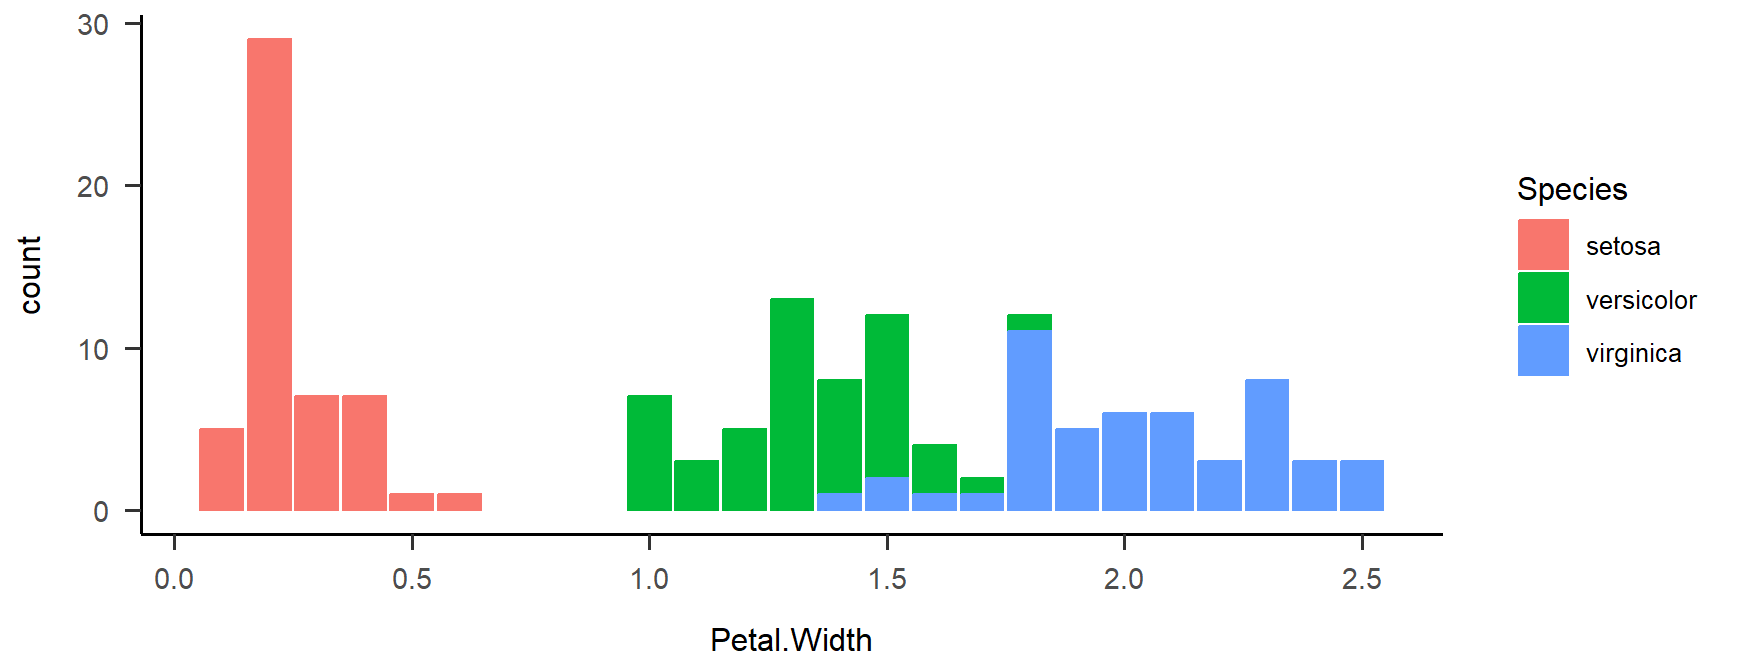
\includegraphics{_main_files/figure-html/unnamed-chunk-37-1} \end{flushleft}

\subsection{Inspiration: colors and palettes}\label{inspiration-colors-and-palettes}

\begin{itemize}
\tightlist
\item
  These plots have all used the default colors from ggplot2
\item
  There are many options for customization, either:

  \begin{itemize}
  \tightlist
  \item
    Use the ``brewer'' palettes from \texttt{ggplot2} with \texttt{scale\_color\_brewer()} or \texttt{scale\_fill\_brewer()}
  \item
    Choose single colors (static aesthetics), check \texttt{colors()} for R color names
  \item
    Create a color palette with all colors that you need and use it with \texttt{scale\_color\_manual()} or \texttt{scale\_fill\_manual()}
  \item
    Use a predefined color palette from packages like \texttt{viridis} or \texttt{unikn} or \texttt{RColorBrewer}\ldots{}
  \end{itemize}
\item
  Have fun with it!
\end{itemize}

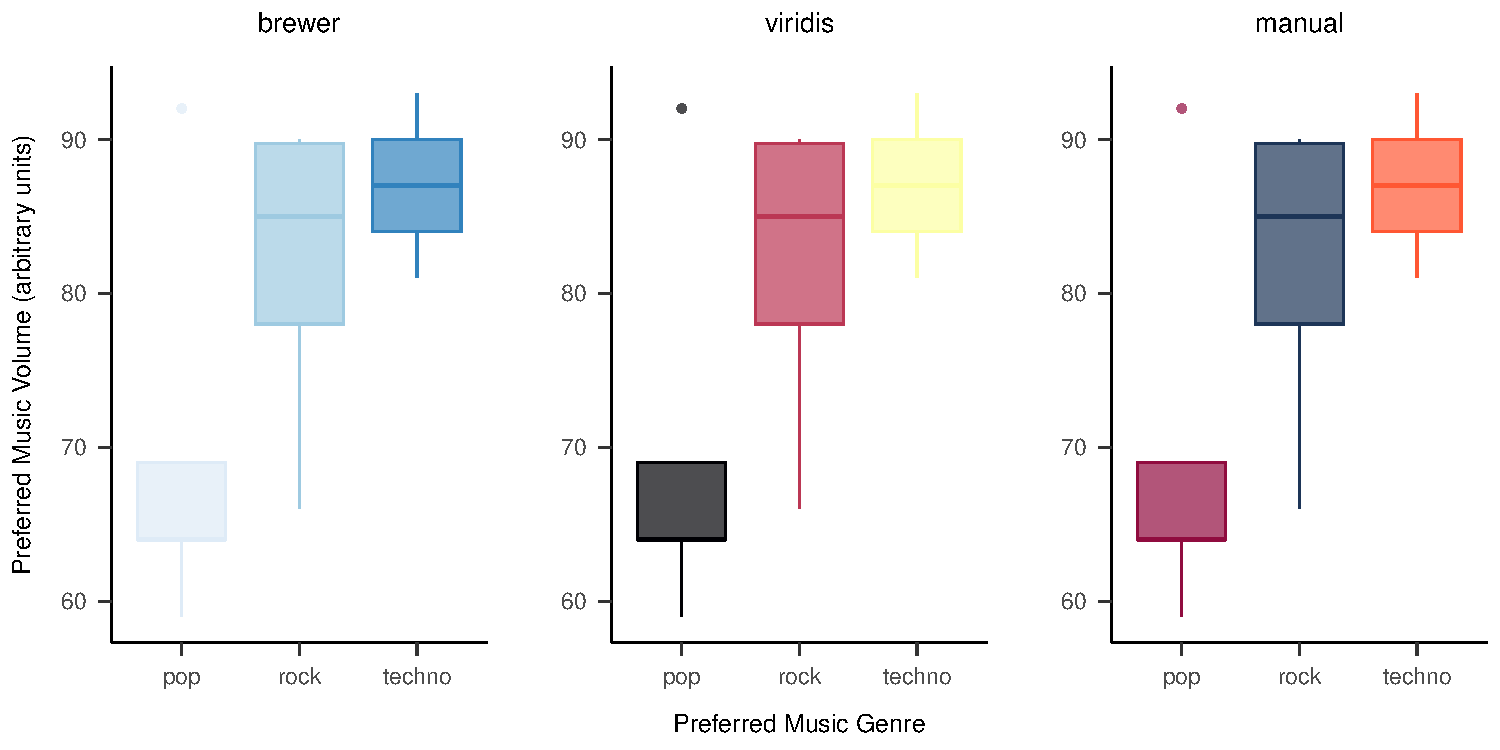
\includegraphics{_main_files/figure-html/unnamed-chunk-38-1.pdf}

\begin{quote}
Showing plots together like this is easy with \texttt{cowplot::plot\_grid()}!
\end{quote}

\section*{Wrap-Up \& Further Resources}\label{wrap-up-further-resources-3}
\addcontentsline{toc}{section}{Wrap-Up \& Further Resources}

\texttt{ggplot2} is a powerful tool for visualizing data

Plot commands are added together with + and executed as one

A basic plot is created with ggplot() + geom\_XYZ(), e.g.~geom\_bar

color \& fill give you nice color options (static \& dynamic)

labs() adds labels to the plot (i.e.~x, y, title, \ldots)

Themes control the background of the plot, e.g.~papaja::theme\_apa() or theme\_minimal()

Color palettes are a great way of elevating a visualization

\href{https://ggplot2.tidyverse.org/articles/ggplot2.html}{ggplot2 vignette}

\href{https://r-graphics.org/}{R Graphics Cookbook}

\href{https://hneth.github.io/unikn/index.html}{unikn}

\href{https://sjmgarnier.github.io/viridisLite/reference/viridis.html}{viridis}

\href{https://www.rdocumentation.org/packages/papaja/versions/0.1.2}{papaja}

\href{https://www.cedricscherer.com/2019/08/05/a-ggplot2-tutorial-for-beautiful-plotting-in-r/}{Beautiful Plotting Guide} Very extensive, I still profit from this guide a lot :)

\href{http://www.sthda.com/english/wiki/ggplot2-colors-how-to-change-colors-automatically-and-manually}{More color palettes explained}

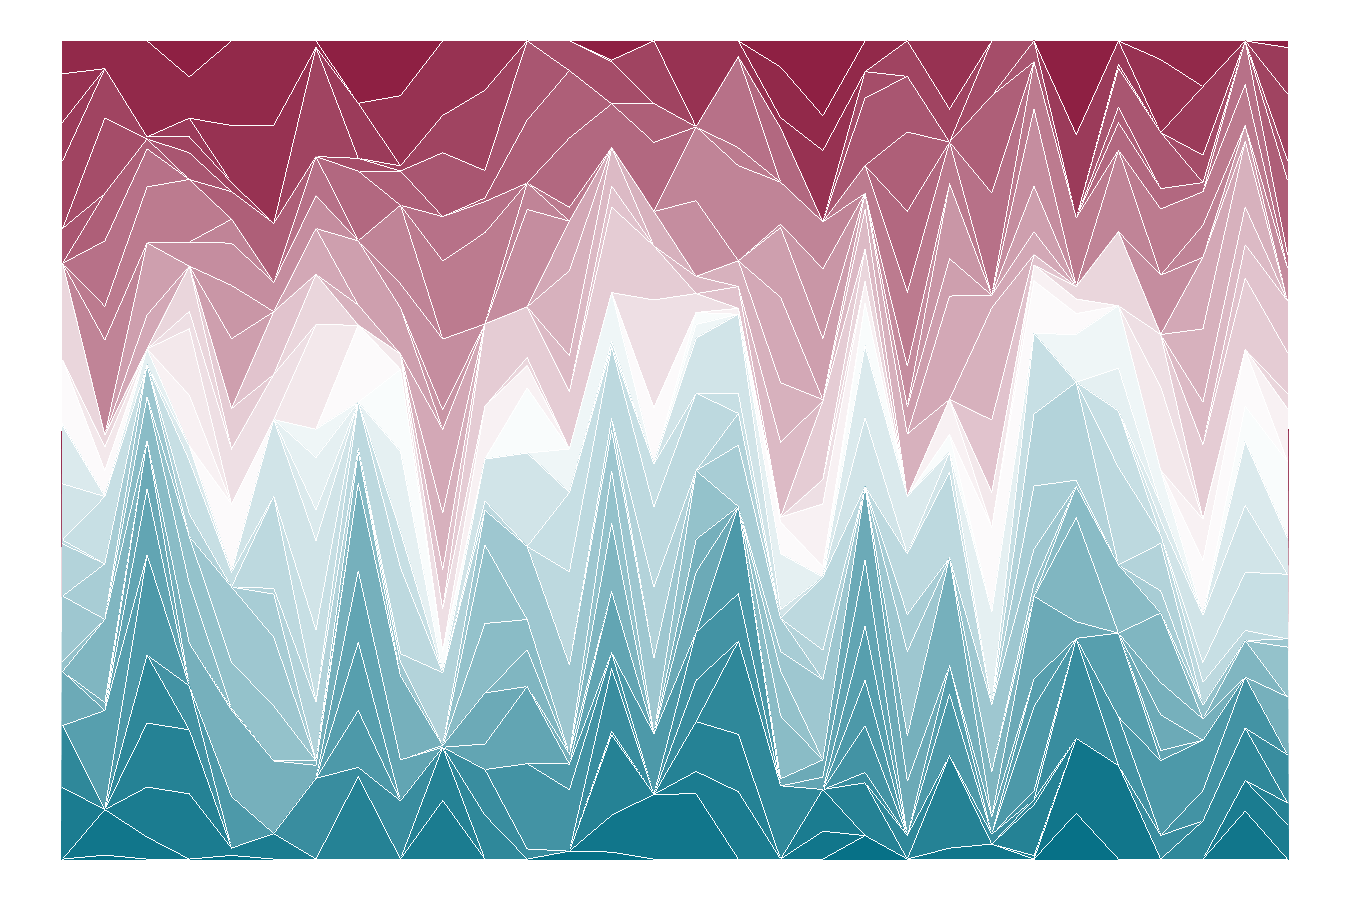
\includegraphics{_main_files/figure-html/unikn-plot-1.pdf}

--\textgreater{}

\part{The Nitty-Gritty}\label{part-the-nitty-gritty}

\chapter{Working with existing Data}\label{exdata}

After learning how to get your data to be the right format and how to look at said data, it now gets down to the nitty-gritty.
In this chapter we will talk about where data can come from and how to get it inside of R.
For that, we will talk about different ways of reading data into R to get the right format and also some first steps that should be taken with data in order to work with it properly.

We will work with some new packages, so please make sure you have the \texttt{readr} package as well as the \texttt{wobblynameR} package, which is only available on GitHub.
To install it, you will first need the \texttt{devtools} package and then use it to install from GitHub:

\begin{Shaded}
\begin{Highlighting}[]
\FunctionTok{install.packages}\NormalTok{(}\StringTok{"devtools"}\NormalTok{)}
\NormalTok{devtools}\SpecialCharTok{::}\FunctionTok{install\_github}\NormalTok{(}\StringTok{"the{-}tave/wobblynameR"}\NormalTok{)}
\end{Highlighting}
\end{Shaded}

\section{Different types of data sources}\label{different-types-of-data-sources}

Data collected from \href{https://www.wextor.eu}{WEXTOR} - like from many other sources - will be exported in the CSV format, which stands for comma-separated values.
That means that this type of data has one row per participant and the values for each column (variable) are separated by a \emph{delimiter} \footnote{\ldots which often times is a comma, but not always! WEXTOR, for example uses semicolons.}.

When our data comes from an Excel file, it will often be exported as CSV because this type of storing data is pretty efficient and uses up very little space on the disk.
A more modern but also more space-consuming way of storing Excel table data is in the XLSX format (Not an acronym, just stands for ``Excel Spreadsheet'').

Many people use SPSS for statistical analysis and creating dataframes.
These data will be stored in a file with the extension SAV.
Generally speaking, SAV files are compatible with R.
However, there are some specialties which can cause problems, such as SPSS labels.
We won't go into depth on this, just know that R can sometimes recognize SPSS labelled variables as their own class, in which case the class of those variables should be corrected manually \footnote{The function calls \texttt{as.numeric()} and \texttt{as.factor()} will suffice in most cases.}.

Finally, of course we can also encounter datafiles that were created in R.
In this case the will have .Rds as the file extension.
A special case of this is when data frames are included in base-R or in a package.
For example, the dataset called \texttt{iris} comes with R as an example dataset.

Therefore, we can run a function on it without having to load it at all:

\begin{Shaded}
\begin{Highlighting}[]
\FunctionTok{head}\NormalTok{(iris)}
\CommentTok{\#   Sepal.Length Sepal.Width Petal.Length Petal.Width Species}
\CommentTok{\# 1          5.1         3.5          1.4         0.2  setosa}
\CommentTok{\# 2          4.9         3.0          1.4         0.2  setosa}
\CommentTok{\# 3          4.7         3.2          1.3         0.2  setosa}
\CommentTok{\# 4          4.6         3.1          1.5         0.2  setosa}
\CommentTok{\# 5          5.0         3.6          1.4         0.2  setosa}
\CommentTok{\# 6          5.4         3.9          1.7         0.4  setosa}
\end{Highlighting}
\end{Shaded}

Depending on which type of data we want to work with, there are different ways of loading the data into R.

\section{Reading in the data}\label{reading-in-the-data}

There are two main ways to load data: via the ``Import Dataset'' menu under the \emph{Environment}-tab or (only) using code and if necessary packages.
In the menu, simply select the option ``Import Dataset'' menu under the top-right \emph{Environment}-tab and use \emph{From text (readr)} for csv or other text files (such as .txt).
Note that this menu also offers the possibility to load data from Excel and SPSS.
However, this is much easier done by just using simple commands directly in your script:

\begin{longtable}[]{@{}ll@{}}
\toprule\noalign{}
Data Source & R command \\
\midrule\noalign{}
\endhead
\bottomrule\noalign{}
\endlastfoot
WEXTOR (CSV) & \texttt{readr::read\_delim("data.csv",\ delim\ =\ ";")} \\
Excel (XLSX) & \texttt{xlsx::read.xlsx("data.xlsx",\ sheetIndex\ =\ 1)} \\
R Data Source (RDS) & \texttt{readRDS("data.Rds")} \\
SPSS (SAV) & \texttt{foreign::read.spss("data.sav")} \\
\end{longtable}

You can follow along these exact code examples if you download the \emph{seminar\_data\_raw} data frame from GitHub and save it in the data subfolder in your R-Project.
You can find it under this link: \url{https://github.com/the-tave/psych_research_in_r/raw/main/data/PsychResearchR_data.csv}.\footnote{If you are connected to the internet anyway you can also use this link as the file path without downloading the data first!}

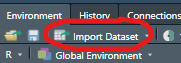
\includegraphics[width=\textwidth,height=0.625in]{./img/import_dataset.png}

Use the ``Import Dataset'' Menu under the \emph{Environment} tab in the upper right corner of R Studio.
In that menu, there are different options for different operations, but for CSV files I recommend the \emph{From Text (readr)} option.
Then we can select our data file and choose some basic aspects of reading in that data.

One of the reasons why i prefer this option over others is that a lot of the times it will recognize the data specifications on its own, so when you have selected the data file on you computer and copy out the generated Code from the Code Preview, it will look something like this:

\subsection*{Generated Code}\label{generated-code}
\addcontentsline{toc}{subsection}{Generated Code}

\begin{Shaded}
\begin{Highlighting}[]
\FunctionTok{library}\NormalTok{(readr)}
\NormalTok{seminar\_data\_raw }\OtherTok{\textless{}{-}} \FunctionTok{read\_delim}\NormalTok{(}\StringTok{"data/seminar\_data\_raw.csv"}\NormalTok{)}
\FunctionTok{View}\NormalTok{(seminar\_data\_raw)}
\end{Highlighting}
\end{Shaded}

The \texttt{read\_delim()} function needs the file path to the data file as the minimum input requirement.
There are many basic edits that can already easily be made in this function, which can also be selected in the menu.
For example, even though ``csv'' stands for \emph{comma-separated values} these tiypes of files sometimes use a semicolon as a delimiter.
When reading in the data, this is sometimes recognized automatically, but when the data looks a bit funky in the preview, making sure the right delimiter is selected is a solid first step.

\begin{figure}
\centering
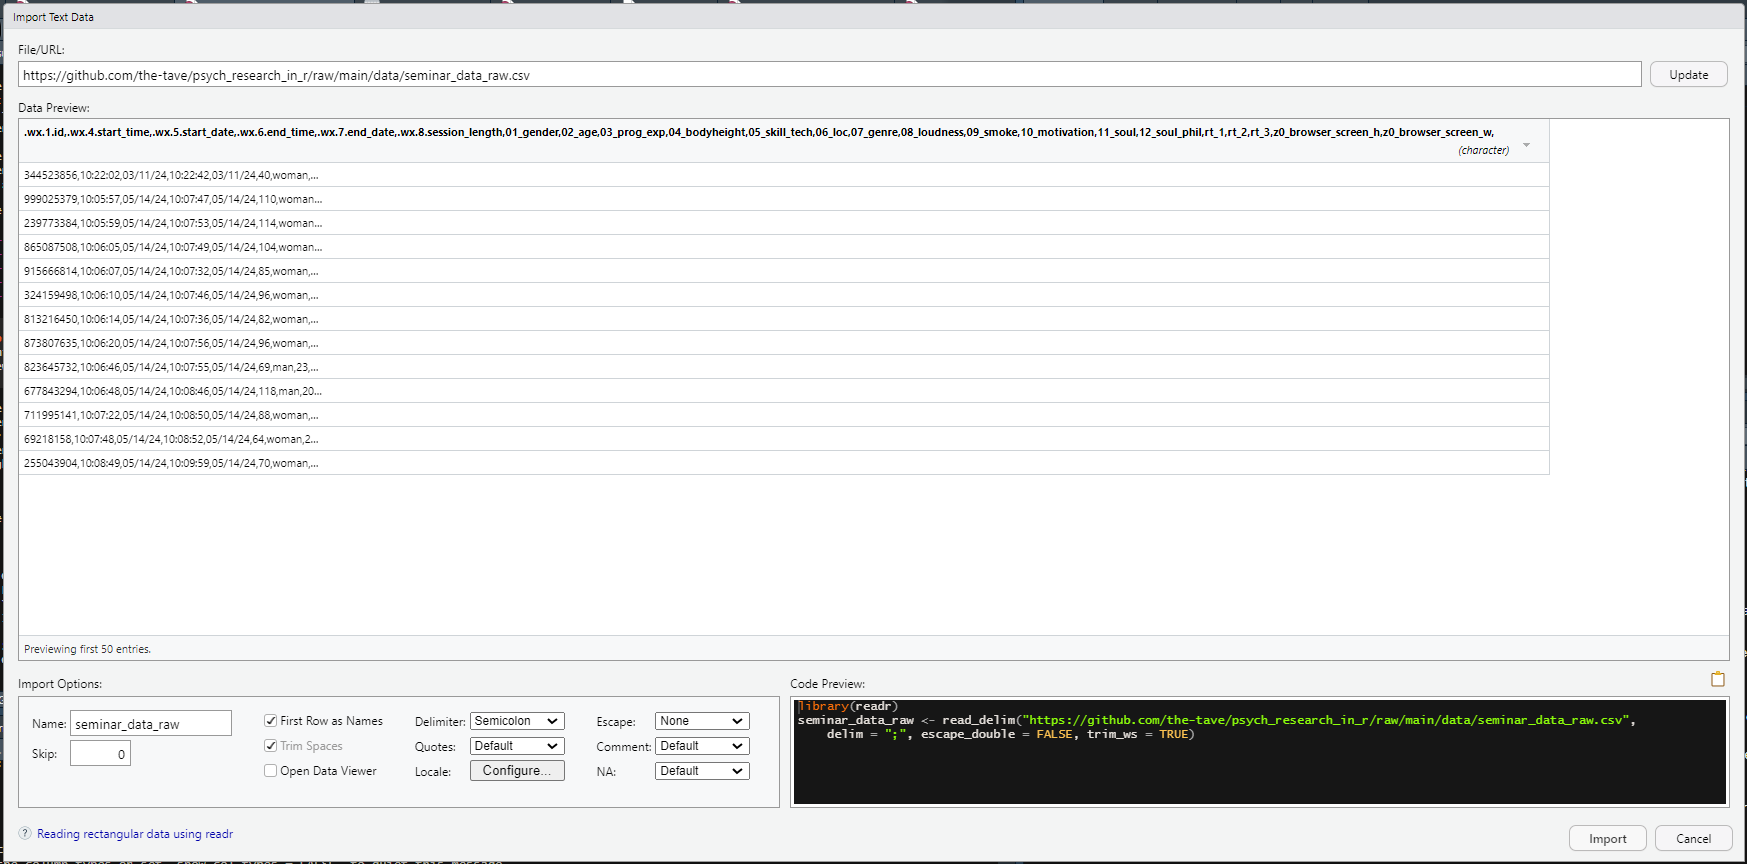
\includegraphics{./img/importcsv.png}
\caption{Example of wonky-looking data in the Import Dataset Menu}
\end{figure}

\subsection*{\texorpdfstring{Basic Edits }{Basic Edits }}\label{basic-edits}
\addcontentsline{toc}{subsection}{Basic Edits }

There are a lot more quite basic edits that we can achieve from the comfort of the Import Dataset menu.
In this case, we will make explicit some specifications that are automatically recognized, namely \texttt{delim\ =\ ","} - i.e.~the correct delimiter, \texttt{escape\_double\ =\ FALSE} - i.e.~double quotes are not treated as a special character\footnote{Escape characters are very important and very confusing. Just know that some special characters can be recognized either as plain text or as a request to do something (as code).} and \texttt{trim\_ws\ =\ TRUE} - i.e.~if there are white spaces in the data, they should be trimmed.

We can also specify some column types in this menu.
Most columns will probably be fine staying the type they are automatically recognized as but especially some date formats are not properly recognized by R.
So it makes sense to look through the data preview and do a quick visual check whether the data you see is displayed properly and the values make sense.
If that check reveals that something is wrong, the little gray triangle next to the variable name offers many column types to choose from and find the one that suits your data.
In our example, we will make sure that the start and end date variables are recognized as dates in the right format.
For that we will choose the \emph{Date} format and trigger a prompt asking for the correct format with some placeholders.
When talking about dates, placeholders like m, d and y should be intuitive enough - suffice it to say that a capital Y stand for the whole year (e.g., 2024) while a small y stands for a shortened year format (e.g., 24).

Another handy column type is \texttt{col\_skip()} which does just that - skip that specific column.
It may seem strange to exclude some data from the get-go, but some data files will end with a delimiter and R recognizes that as another column.
This is also the case for this data file from \href{https://www.wextor.eu}{WEXTOR}, which is why we will skip the last column (which is completely empty).

Moreover, we can take full advantage of both menu and script by copying the code that is generated from the menu into our script.
This automatically gives us a nice structure to start a new script for analyses with a first library command at the top (for \texttt{readr}) and reading in the data as a first step of analysis.
As a best practice, we will change the name of our raw data set in R to ``raw''.
This data set can remain untouched throughout all other data munging steps which allows us to revise edits or go back a step if something goes wrong with having to reload the data (especially with a big data set, reading it in can take a bit of time).

As a last first step, we will use the \texttt{namepref0()} (``name-prefix-zero'') function from the \texttt{wobblynameR} package to add the prefix ``v'' to every variable name.
There are different reasons why a consistent prefix might be useful - in this case the variable names start with a number, which can cause problems in R.
The function takes the whole data frame as input and outputs that data frame with all variables renamed, which we will save in a new data frame called ``seminar''.
The resulting code - the first part of which can be completely generated by the menu - looks like this:

\subsection*{Result}\label{result}
\addcontentsline{toc}{subsection}{Result}

\begin{Shaded}
\begin{Highlighting}[]
\CommentTok{\# Library commands on top}
\FunctionTok{library}\NormalTok{(readr)}
\FunctionTok{library}\NormalTok{(wobblynameR)}

\CommentTok{\# Generated code}
\NormalTok{raw }\OtherTok{\textless{}{-}} \FunctionTok{read\_delim}\NormalTok{(}\StringTok{"./data/seminar\_data\_raw.csv"}\NormalTok{, }
    \AttributeTok{delim =} \StringTok{","}\NormalTok{, }\AttributeTok{escape\_double =} \ConstantTok{FALSE}\NormalTok{, }
    \AttributeTok{col\_types =} \FunctionTok{cols}\NormalTok{(}\AttributeTok{.wx.5.start\_date =} \FunctionTok{col\_date}\NormalTok{(}\AttributeTok{format =} \StringTok{"\%m/\%d/\%y"}\NormalTok{),}
                     \AttributeTok{.wx.7.end\_date =} \FunctionTok{col\_date}\NormalTok{(}\AttributeTok{format =} \StringTok{"\%m/\%d/\%y"}\NormalTok{), }
                     \AttributeTok{...24 =} \FunctionTok{col\_skip}\NormalTok{()),}
    \AttributeTok{trim\_ws =} \ConstantTok{TRUE}\NormalTok{)}

\CommentTok{\# Add "v" as varname prefix to all variables}
\NormalTok{seminar }\OtherTok{\textless{}{-}} \FunctionTok{namepref0}\NormalTok{(raw, }\StringTok{"v"}\NormalTok{)}
\end{Highlighting}
\end{Shaded}

\section{Codebook}\label{codebook}

In my experience, it is easiest to work with data where you have an idea of what to expect.
Even if you create your survey or experiment, you may forget what exactly is in which variable.
With the \texttt{str()} function we can get a solid overview of the data structure and with \texttt{names(seminar)} R will output all variable names in the seminar data frame.

When you work with someone's data, it is a good idea to either consult their codebook.
It might also help you in deciding what type of analyses might make sense with which variables.

\section{Descriptives}\label{descriptives}

Next to the general overview of what is contained in the data, descriptive statistics are very useful to look at for the variables of interest.
Also, in any report, we need to give our readers or listeners an overview of the data to better judge the actual meaning of the results.
Basically, we need to know the sample to judge the results!
A sample of e.g.~10 female psychology students probably shows different results - generally speaking - than a sample of 10 male soldiers.

Name some common descriptive statistics:

\begin{itemize}
\item
  \begin{center}\rule{0.5\linewidth}{0.5pt}\end{center}
\item
  \begin{center}\rule{0.5\linewidth}{0.5pt}\end{center}
\item
  \begin{center}\rule{0.5\linewidth}{0.5pt}\end{center}
\item
  \begin{center}\rule{0.5\linewidth}{0.5pt}\end{center}
\item
  \begin{center}\rule{0.5\linewidth}{0.5pt}\end{center}
\end{itemize}

Show the solutions

\begin{itemize}
\tightlist
\item
  Mean
\item
  Median
\item
  Mode
\item
  Variability, Variance, Standard Deviation
\item
  Data Visualization\ldots{}
\end{itemize}

\subsection{group\_by \& summarize}\label{group_by-summarize-1}

With the \texttt{dplyr}-workflow, we can easily output group statistics with the keywords: \texttt{group\_by()} and \texttt{summarize()}
The code is built like any other \texttt{dplyr} workflow with pipes ( \%\textgreater\% ) in between each function.
Commonly, you will first define the name of the data frame - in the first example we will use the \texttt{iris} data.
Then choose the variable that should be used for grouping, such as gender or in this case \emph{Species}.
Make sure that this variable is recognized as either a factor or character and try to choose a variable that has not too many groups, otherwise it might get too crowded and confusing rather than helpful.
Then you can pipe this grouped data into the summarize function and define some names for the measures that will we used in the output as well as the measure you would like to use - i.e.~commonly \texttt{mean()} \texttt{median()} or \texttt{sd()}.
You can also use \texttt{n()} to display the group sizes.

\begin{Shaded}
\begin{Highlighting}[]
\NormalTok{iris }\SpecialCharTok{\%\textgreater{}\%} 
  \FunctionTok{group\_by}\NormalTok{(Species) }\SpecialCharTok{\%\textgreater{}\%} 
  \FunctionTok{summarize}\NormalTok{(}\AttributeTok{m\_plength =} \FunctionTok{mean}\NormalTok{(Petal.Length),}
            \AttributeTok{med\_pwidth =} \FunctionTok{median}\NormalTok{(Petal.Width),}
            \AttributeTok{m\_slength =} \FunctionTok{mean}\NormalTok{(Sepal.Length),}
            \AttributeTok{mode\_swidth =} \FunctionTok{getmode}\NormalTok{(Sepal.Width),}
            \AttributeTok{n =} \FunctionTok{n}\NormalTok{())}
\CommentTok{\# \# A tibble: 3 x 6}
\CommentTok{\#   Species    m\_plength med\_pwidth m\_slength mode\_swidth     n}
\CommentTok{\#   \textless{}fct\textgreater{}          \textless{}dbl\textgreater{}      \textless{}dbl\textgreater{}     \textless{}dbl\textgreater{}       \textless{}dbl\textgreater{} \textless{}int\textgreater{}}
\CommentTok{\# 1 setosa          1.46        0.2      5.01         3.4    50}
\CommentTok{\# 2 versicolor      4.26        1.3      5.94         3      50}
\CommentTok{\# 3 virginica       5.55        2        6.59         3      50}
\end{Highlighting}
\end{Shaded}

\section{Missing Data}\label{missing-data}

In R, missing data or \texttt{NA}s (which stands for ``Not Available'') occur when some values in your dataset are absent or not recorded.
This is important to note because missing data can affect your analyses and the conclusions you draw from your research.
R treats these missing values as a special case, so they don't interfere with calculations in the same way as other values.
You can identify missing data using functions like \texttt{is.na()}, and there are various methods to handle them, such as removing rows with missing values or using statistical techniques to estimate them.

This can easily be done with the \texttt{dplyr} tools we already know and a bit of logic:
If a variable \emph{X} in the data set \emph{data} has one or more missing values, you can use

\begin{Shaded}
\begin{Highlighting}[]
\NormalTok{data\_edited }\OtherTok{\textless{}{-}}\NormalTok{ data }\SpecialCharTok{|\textgreater{}} 
  \FunctionTok{filter}\NormalTok{(}\SpecialCharTok{!}\FunctionTok{is.na}\NormalTok{(X))}
\end{Highlighting}
\end{Shaded}

to filter in only those rows in the variable that as \emph{not} NA (thus the !).
Handling missing data properly ensures that your analysis is accurate and reliable.

\section*{Exercises}\label{exercises-2}
\addcontentsline{toc}{section}{Exercises}

\subsection*{group\_by \& summarize}\label{group_by-summarize-2}
\addcontentsline{toc}{subsection}{group\_by \& summarize}

Follow the structure to group the edited seminar data by belief in the soul and output a summary with

\begin{itemize}
\tightlist
\item
  mean age
\item
  mean technological skill
\item
  mode music genre
\item
  median volume of music
\item
  grouped n (function \emph{n()})
\end{itemize}

Solution

\begin{Shaded}
\begin{Highlighting}[]
\NormalTok{seminar }\SpecialCharTok{\%\textgreater{}\%} 
  \FunctionTok{group\_by}\NormalTok{(v11\_soul) }\SpecialCharTok{\%\textgreater{}\%} 
  \FunctionTok{summarize}\NormalTok{(}\AttributeTok{m\_age =} \FunctionTok{mean}\NormalTok{(v02\_age),}
            \AttributeTok{m\_tech\_skill =} \FunctionTok{mean}\NormalTok{(v05\_skill\_tech),}
            \AttributeTok{mode\_music =} \FunctionTok{getmode}\NormalTok{(v07\_genre),}
            \AttributeTok{median\_volume =} \FunctionTok{median}\NormalTok{(v08\_loudness),}
            \AttributeTok{n =} \FunctionTok{n}\NormalTok{())}
\CommentTok{\# \# A tibble: 3 x 6}
\CommentTok{\#   v11\_soul m\_age m\_tech\_skill mode\_music median\_volume     n}
\CommentTok{\#   \textless{}chr\textgreater{}    \textless{}dbl\textgreater{}        \textless{}dbl\textgreater{} \textless{}chr\textgreater{}              \textless{}dbl\textgreater{} \textless{}int\textgreater{}}
\CommentTok{\# 1 dunno     23.4         29.4 techno              89       5}
\CommentTok{\# 2 no        22           45   pop                 74.5     2}
\CommentTok{\# 3 yes       22.5         42   rock                67.5     6}
\end{Highlighting}
\end{Shaded}

\subsection*{Prepare seminar data}\label{prepare-seminar-data}
\addcontentsline{toc}{subsection}{Prepare seminar data}

We have read in the ``seminar\_data\_raw'' and looked at some of the basic edits that we can do easily.
However, in order to be able to work with the dataset in easily in the future, we should do some more advanced edits.
Specifically, we will:

\begin{enumerate}
\def\labelenumi{\arabic{enumi}.}
\tightlist
\item
  Change the date format so we get a start and end variable including time and date instead of separate date and time variables
\item
  Remove the unnecessary original date and time variables
\item
  Change the one missing value in \texttt{v12\_soul\_phil} to ``dunno''
\item
  Rename the ID variable to \texttt{ID} \& session length variable to \texttt{session\_length}
\item
  Make our data type explicit using \texttt{as.data.frame()}
\item
  Save our edited data in an R data set (\texttt{Rds}) format so we can use it more easily later!
\end{enumerate}

I suggest using some of the \texttt{dplyr} commands that were introduced in the last chapter for edits 1 through 4.
You can try to figure them out on your own and later look at the solution below.
\textbf{I highly recommend you follow along with these steps, as we will use this dataset in later chapters}\footnote{This is very close to real-life practice, but you can also skip it and download the Rds-file from the GitHub repository \href{https://github.com/the-tave/psych_research_in_r/blob/main/data/seminar_data.Rds}{here}.}

Solution

\begin{Shaded}
\begin{Highlighting}[]
\NormalTok{seminar }\OtherTok{\textless{}{-}}\NormalTok{ seminar }\SpecialCharTok{|\textgreater{}} 
  \CommentTok{\# 1. Change date format }
  \FunctionTok{mutate}\NormalTok{(}\AttributeTok{start =} \FunctionTok{as.POSIXct}\NormalTok{(}\FunctionTok{paste}\NormalTok{(v.wx.}\FloatTok{5.}\NormalTok{start\_date, v.wx.}\FloatTok{4.}\NormalTok{start\_time), }\AttributeTok{format =} \StringTok{"\%Y{-}\%m{-}\%d \%H:\%M:\%S"}\NormalTok{),}
         \AttributeTok{end =} \FunctionTok{as.POSIXct}\NormalTok{(}\FunctionTok{paste}\NormalTok{(v.wx.}\FloatTok{7.}\NormalTok{end\_date, v.wx.}\FloatTok{6.}\NormalTok{end\_time), }\AttributeTok{format =} \StringTok{"\%Y{-}\%m{-}\%d \%H:\%M:\%S"}\NormalTok{), }
         \AttributeTok{.before =}\NormalTok{ v01\_gender) }\SpecialCharTok{\%\textgreater{}\%} \CommentTok{\# it is more efficient to have date and time together}
  \CommentTok{\# 2. Remove (now) unnecessary original date vars }
  \FunctionTok{select}\NormalTok{(}\SpecialCharTok{{-}}\FunctionTok{c}\NormalTok{(v.wx.}\FloatTok{4.}\NormalTok{start\_time, v.wx.}\FloatTok{5.}\NormalTok{start\_date, v.wx.}\FloatTok{6.}\NormalTok{end\_time, v.wx.}\FloatTok{7.}\NormalTok{end\_date)) }\SpecialCharTok{\%\textgreater{}\%} 
  \CommentTok{\# 3. Change missing value to "don\textquotesingle{}t know" {-} in this case makes sense in context}
  \FunctionTok{mutate}\NormalTok{(}\AttributeTok{v12\_soul\_phil =} \FunctionTok{ifelse}\NormalTok{(}\FunctionTok{is.na}\NormalTok{(v12\_soul\_phil), }\StringTok{"dunno"}\NormalTok{, v12\_soul\_phil)) }\SpecialCharTok{|\textgreater{}} 
  \CommentTok{\# 4. Rename the ID \& session length variable}
  \FunctionTok{rename}\NormalTok{(}\AttributeTok{ID =}\NormalTok{ v.wx.}\FloatTok{1.}\NormalTok{id,}
         \AttributeTok{session\_length =}\NormalTok{ v.wx.}\FloatTok{8.}\NormalTok{session\_length)}

\CommentTok{\# 5. Make data type explicit}
\NormalTok{seminar }\OtherTok{\textless{}{-}} \FunctionTok{as.data.frame}\NormalTok{(seminar)}

\CommentTok{\# 6. Save edited data frame in Rds format}
\FunctionTok{saveRDS}\NormalTok{(seminar, }\StringTok{"./data/seminar\_data.Rds"}\NormalTok{)}
\end{Highlighting}
\end{Shaded}

\section*{Wrap-Up \& Further Resources}\label{wrap-up-further-resources-4}
\addcontentsline{toc}{section}{Wrap-Up \& Further Resources}

Reading in data works with commands like readRDS() but also the ``Import Dataset'' Menu

Use the menu for WEXTOR data to get an overview and reproducible code

Get/ create a codebook for your data

Always report descriptive data

dplyr's \texttt{group\_by()} and \texttt{summarize()} can output grouped descriptives

\href{https://www.datafiles.samhsa.gov/get-help/format-specific-issues/how-do-i-read-data-r}{Reading in Data in Different Formats}

\href{https://statsandr.com/blog/descriptive-statistics-in-r/}{Stats and R: Descriptives}

\chapter{Loops and Conditionals}\label{loops-and-conditionals}

\section{What is a loop?}\label{what-is-a-loop}

\begin{itemize}
\tightlist
\item
  Loops are automations that take care of repetitive tasks

  \begin{itemize}
  \tightlist
  \item
    Typically, we might go through data row by row and perform a task
  \end{itemize}
\item
  Loops can have different forms:

  \begin{itemize}
  \tightlist
  \item
    \textbf{for}: loop over a pre-defined set of values, such as a number sequence
  \item
    \textbf{while}: define constraints and keep loop running as long as they are met
  \item
    \textbf{repeat}: loop repeats until broken (\emph{I do not recommend this ever!})
  \end{itemize}
\item
  For is most common, while is nice for more advanced simulations
\end{itemize}

\subsection{What are conditionals?}\label{what-are-conditionals}

\begin{itemize}
\tightlist
\item
  Conditionals define different actions for different conditions
\item
  They follow intuitive language:

  \begin{itemize}
  \tightlist
  \item
    \textbf{if}: define action to take when condition is met (logical)
  \item
    \textbf{else if}: defince action for another condition
  \item
    \textbf{else}: define action for everything else
  \end{itemize}
\item
  \textbf{ifelse} is the shortcut-function we already got to know for recoding with \texttt{mutate()}

  \begin{itemize}
  \tightlist
  \item
    defines exactly 1 condition, 1 action, 1 alternative
  \item
    expandable version of ifelse is case\_when
  \end{itemize}
\end{itemize}

\section{Exercise: What should I use?}\label{exercise-what-should-i-use}

\begin{enumerate}
\def\labelenumi{\arabic{enumi}.}
\tightlist
\item
  I want to print numbers from 1 to 7!

  \begin{itemize}
  \tightlist
  \item
    for loop (but realistically \emph{1:7} ;) )
  \end{itemize}
\item
  I need to simulate more data as long as my sample size is smaller than 200!

  \begin{itemize}
  \tightlist
  \item
    while loop
  \end{itemize}
\item
  I want to print the age of only the females in my sample!

  \begin{itemize}
  \tightlist
  \item
    if/ else
  \end{itemize}
\end{enumerate}

\section{for-loop}\label{for-loop}

\begin{itemize}
\tightlist
\item
  In a for loop, we need to define the range \emph{for} which the loop should run
\item
  We define an \emph{iterating variable} that will change each time the loop runs and take on all values of the defined range

  \begin{itemize}
  \tightlist
  \item
    Typically, we call this variable ``i''
  \end{itemize}
\item
  We define the range in round brackets and all actions the loop should take in curly brackets
\end{itemize}

\subsection{Example}\label{example}

\begin{Shaded}
\begin{Highlighting}[]
\ControlFlowTok{for}\NormalTok{(i }\ControlFlowTok{in} \DecValTok{1}\SpecialCharTok{:}\DecValTok{4}\NormalTok{)\{}
  \FunctionTok{print}\NormalTok{(}\FunctionTok{paste}\NormalTok{(}\StringTok{"The iteration is"}\NormalTok{, i))}
\NormalTok{\}}
\CommentTok{\# [1] "The iteration is 1"}
\CommentTok{\# [1] "The iteration is 2"}
\CommentTok{\# [1] "The iteration is 3"}
\CommentTok{\# [1] "The iteration is 4"}
\end{Highlighting}
\end{Shaded}

\subsection{Conditionals: If - else}\label{conditionals-if---else}

\begin{Shaded}
\begin{Highlighting}[]
\ControlFlowTok{if}\NormalTok{(variable }\SpecialCharTok{==} \StringTok{"value"}\NormalTok{)\{}
  \FunctionTok{print}\NormalTok{(}\StringTok{"Do something"}\NormalTok{)}
\NormalTok{\} }\ControlFlowTok{else} \ControlFlowTok{if}\NormalTok{(variable }\SpecialCharTok{==} \StringTok{"other\_value"}\NormalTok{)\{}
  \FunctionTok{print}\NormalTok{(}\StringTok{"Do some other thing"}\NormalTok{)}
\NormalTok{\} }\ControlFlowTok{else}\NormalTok{ \{}
  \FunctionTok{print}\NormalTok{(}\StringTok{"Do anything else"}\NormalTok{)}
\NormalTok{\}}
\end{Highlighting}
\end{Shaded}

\subsection{Conditionals: If - else}\label{conditionals-if---else-1}

\subsubsection{Checking numbers \textbar{}}\label{checking-numbers}

We want to test whether numbers in a loop are divisible by 3. If they are, we will display ``Divisible by 3'', and if not, we will simply output the iteration number like before.

For that we will use the modulo \%\% , which gives us the rest of a division. Let's try it out!

\begin{Shaded}
\begin{Highlighting}[]
\ControlFlowTok{for}\NormalTok{(i }\ControlFlowTok{in} \DecValTok{1}\SpecialCharTok{:}\DecValTok{4}\NormalTok{)\{}
  \ControlFlowTok{if}\NormalTok{(i }\SpecialCharTok{\%\%} \DecValTok{3} \SpecialCharTok{==} \DecValTok{0}\NormalTok{)\{}
    \FunctionTok{print}\NormalTok{(}\StringTok{"Divisible by 3!"}\NormalTok{)}
\NormalTok{  \} }\ControlFlowTok{else}\NormalTok{ \{}
    \FunctionTok{print}\NormalTok{(i) }
\NormalTok{  \}}
\NormalTok{\}}
\CommentTok{\# [1] 1}
\CommentTok{\# [1] 2}
\CommentTok{\# [1] "Divisible by 3!"}
\CommentTok{\# [1] 4}
\end{Highlighting}
\end{Shaded}

\subsection{Exercise}\label{exercise-2}

Use a for-loop to display your favorite numbers.
The numbers should be between 10 and 25.

If the number is divisible completely by 5, you should output ``Divisible by 5!'', if not please output the iteration number only.

Solution

\begin{Shaded}
\begin{Highlighting}[]
\ControlFlowTok{for}\NormalTok{(i }\ControlFlowTok{in} \DecValTok{10}\SpecialCharTok{:}\DecValTok{25}\NormalTok{)\{}
  \ControlFlowTok{if}\NormalTok{(i }\SpecialCharTok{\%\%} \DecValTok{5} \SpecialCharTok{==} \DecValTok{0}\NormalTok{)\{}
    \FunctionTok{print}\NormalTok{(}\StringTok{"Divisible by 5!"}\NormalTok{)}
\NormalTok{  \} }\ControlFlowTok{else}\NormalTok{ \{}
    \FunctionTok{print}\NormalTok{(i) }
\NormalTok{  \}}
\NormalTok{\}}
\CommentTok{\# [1] "Divisible by 5!"}
\CommentTok{\# [1] 11}
\CommentTok{\# [1] 12}
\CommentTok{\# [1] 13}
\CommentTok{\# [1] 14}
\CommentTok{\# [1] "Divisible by 5!"}
\CommentTok{\# [1] 16}
\CommentTok{\# [1] 17}
\CommentTok{\# [1] 18}
\CommentTok{\# [1] 19}
\CommentTok{\# [1] "Divisible by 5!"}
\CommentTok{\# [1] 21}
\CommentTok{\# [1] 22}
\CommentTok{\# [1] 23}
\CommentTok{\# [1] 24}
\CommentTok{\# [1] "Divisible by 5!"}
\end{Highlighting}
\end{Shaded}

\section{Same function, different variables}\label{same-function-different-variables}

\begin{Shaded}
\begin{Highlighting}[]
\ControlFlowTok{for}\NormalTok{(i }\ControlFlowTok{in} \FunctionTok{c}\NormalTok{(}\StringTok{"Sepal.Length"}\NormalTok{, }\StringTok{"Sepal.Width"}\NormalTok{, }\StringTok{"Petal.Length"}\NormalTok{, }\StringTok{"Petal.Width"}\NormalTok{))\{}
  \FunctionTok{print}\NormalTok{(}\FunctionTok{mean}\NormalTok{(iris[ , i]))}
\NormalTok{\}}
\CommentTok{\# [1] 5.843333}
\CommentTok{\# [1] 3.057333}
\CommentTok{\# [1] 3.758}
\CommentTok{\# [1] 1.199333}
\end{Highlighting}
\end{Shaded}

Brainteaser : What is the class() of i here?

\begin{itemize}
\tightlist
\item
  character
\end{itemize}

\subsection{More sophisticated}\label{more-sophisticated}

\begin{Shaded}
\begin{Highlighting}[]
\NormalTok{vector }\OtherTok{\textless{}{-}} \FunctionTok{c}\NormalTok{(}\StringTok{"Sepal.Length"}\NormalTok{, }\StringTok{"Sepal.Width"}\NormalTok{, }\StringTok{"Petal.Length"}\NormalTok{, }\StringTok{"Petal.Width"}\NormalTok{)}

\ControlFlowTok{for}\NormalTok{(i }\ControlFlowTok{in} \DecValTok{1}\SpecialCharTok{:}\FunctionTok{length}\NormalTok{(vector))\{}
  \FunctionTok{print}\NormalTok{(}\FunctionTok{paste}\NormalTok{(}\StringTok{"The mean value of"}\NormalTok{, vector[i], }\StringTok{"is"}\NormalTok{, }
              \FunctionTok{round}\NormalTok{(}\FunctionTok{mean}\NormalTok{(iris[ , vector[i]]), }\DecValTok{2}\NormalTok{)))}
\NormalTok{\}}
\CommentTok{\# [1] "The mean value of Sepal.Length is 5.84"}
\CommentTok{\# [1] "The mean value of Sepal.Width is 3.06"}
\CommentTok{\# [1] "The mean value of Petal.Length is 3.76"}
\CommentTok{\# [1] "The mean value of Petal.Width is 1.2"}
\end{Highlighting}
\end{Shaded}

Brainteaser : And what is the class() of i now?

\begin{itemize}
\tightlist
\item
  integer (numeric)
\end{itemize}

\subsection{With saving values}\label{with-saving-values}

\begin{Shaded}
\begin{Highlighting}[]
\NormalTok{vector }\OtherTok{\textless{}{-}} \FunctionTok{c}\NormalTok{(}\StringTok{"Sepal.Length"}\NormalTok{, }\StringTok{"Sepal.Width"}\NormalTok{, }\StringTok{"Petal.Length"}\NormalTok{, }\StringTok{"Petal.Width"}\NormalTok{)}
\NormalTok{means }\OtherTok{\textless{}{-}} \FunctionTok{rep}\NormalTok{(}\ConstantTok{NA}\NormalTok{, }\FunctionTok{length}\NormalTok{(vector)) }\CommentTok{\# create "empty" vector to fill}

\ControlFlowTok{for}\NormalTok{(i }\ControlFlowTok{in} \DecValTok{1}\SpecialCharTok{:}\FunctionTok{length}\NormalTok{(vector))\{}
  \FunctionTok{print}\NormalTok{(}\FunctionTok{paste}\NormalTok{(}\StringTok{"The mean value of"}\NormalTok{, vector[i], }\StringTok{"is"}\NormalTok{, }
              \FunctionTok{round}\NormalTok{(}\FunctionTok{mean}\NormalTok{(iris[ , vector[i]]), }\DecValTok{2}\NormalTok{)))}
\NormalTok{  means[i] }\OtherTok{\textless{}{-}} \FunctionTok{round}\NormalTok{(}\FunctionTok{mean}\NormalTok{(iris[ , vector[i]]), }\DecValTok{2}\NormalTok{)}
\NormalTok{\}}
\CommentTok{\# [1] "The mean value of Sepal.Length is 5.84"}
\CommentTok{\# [1] "The mean value of Sepal.Width is 3.06"}
\CommentTok{\# [1] "The mean value of Petal.Length is 3.76"}
\CommentTok{\# [1] "The mean value of Petal.Width is 1.2"}
\end{Highlighting}
\end{Shaded}

\subsection{Exercise: Seminar Data}\label{exercise-seminar-data}

Please download an edited version of our seminar data from ILIAS. You will find it under \emph{data} as a zip folder. The dataset in it should have ``.Rds'' as a file ending. Read it in using:

\begin{Shaded}
\begin{Highlighting}[]
\NormalTok{seminar }\OtherTok{\textless{}{-}} \FunctionTok{readRDS}\NormalTok{(}\StringTok{"./data/seminar\_data.Rds"}\NormalTok{)}
\end{Highlighting}
\end{Shaded}

\textbf{Create a for-loop that saves the means of age, body height and technological skill from that seminar data in a vector named ``seminar\_means''.}

Hint: I renamed the variables to make them nicer to work with, so check out names(seminar)!

\subsection{Solution}\label{solution-1}

\begin{Shaded}
\begin{Highlighting}[]
\NormalTok{vector }\OtherTok{\textless{}{-}} \FunctionTok{c}\NormalTok{(}\StringTok{"v02\_age"}\NormalTok{, }\StringTok{"v04\_bodyheight"}\NormalTok{, }\StringTok{"v05\_skill\_tech"}\NormalTok{)}
\NormalTok{seminar\_means }\OtherTok{\textless{}{-}} \FunctionTok{rep}\NormalTok{(}\ConstantTok{NA}\NormalTok{, }\FunctionTok{length}\NormalTok{(vector)) }\CommentTok{\# create "empty" vector to fill}

\ControlFlowTok{for}\NormalTok{(i }\ControlFlowTok{in} \DecValTok{1}\SpecialCharTok{:}\FunctionTok{length}\NormalTok{(vector))\{}
\NormalTok{  seminar\_means[i] }\OtherTok{\textless{}{-}} \FunctionTok{round}\NormalTok{(}\FunctionTok{mean}\NormalTok{(seminar[ , vector[i]]), }\DecValTok{2}\NormalTok{)}
\NormalTok{\}}
\end{Highlighting}
\end{Shaded}

\subsection{Checking What's Going On}\label{checking-whats-going-on}

\subsubsection{browser()}\label{browser}

\begin{itemize}
\tightlist
\item
  In order to break our loop and enter a ``debugging'' mode, we can add browser() to any loop like so:
\end{itemize}

\begin{Shaded}
\begin{Highlighting}[]
\NormalTok{vector }\OtherTok{\textless{}{-}} \FunctionTok{c}\NormalTok{(}\StringTok{"v02\_age"}\NormalTok{, }\StringTok{"v04\_bodyheight"}\NormalTok{, }\StringTok{"v05\_skill\_tech"}\NormalTok{)}
\NormalTok{seminar\_means }\OtherTok{\textless{}{-}} \FunctionTok{rep}\NormalTok{(}\ConstantTok{NA}\NormalTok{, }\FunctionTok{length}\NormalTok{(vector)) }\CommentTok{\# create "empty" vector to fill}

\ControlFlowTok{for}\NormalTok{(i }\ControlFlowTok{in} \DecValTok{1}\SpecialCharTok{:}\FunctionTok{length}\NormalTok{(vector))\{}
\NormalTok{  seminar\_means[i] }\OtherTok{\textless{}{-}} \FunctionTok{round}\NormalTok{(}\FunctionTok{mean}\NormalTok{(seminar[ , vector[i]]), }\DecValTok{2}\NormalTok{)}
  \FunctionTok{browser}\NormalTok{()}
\NormalTok{\}}
\end{Highlighting}
\end{Shaded}

\begin{itemize}
\item
  The loop will run the first iteration until browser is called and then pause
\item
  It allows you to check in the console whether all variables look the way you want them to without having to wait for the loop to run

  \begin{itemize}
  \tightlist
  \item
    Or if there are errors/ warnings, you can check \emph{when} they occur by moving the browser() to a different location in the code
  \end{itemize}
\item
  To continue with the next iteration while in browser, type ``c'' into the console, ``Q'' to quit

  \begin{itemize}
  \tightlist
  \item
    The Esc key will also terminate the browser
  \end{itemize}
\item
  \textbf{Make sure you exit it} before continuing with anything else
\end{itemize}

\section{Loop with Conditional}\label{loop-with-conditional}

In our seminar data, the \textbf{average body height is 167.23 cm}. We want to create a loop that goes through all rows (all seminar students) and outputs their height and whether it is above or below average.

What do we need for that?

\subsection{Elements}\label{elements}

\begin{itemize}
\tightlist
\item
  For each person:
\item
  Check \emph{if} their body height is above average

  \begin{itemize}
  \tightlist
  \item
    If yes: Output ``This person is taller than average with \ldots{}''
  \item
    Else: Output ``This person is less tall than average with\ldots{}''
  \end{itemize}
\item
  Then paste the person's body height
\item
  Loop that over each person!
\end{itemize}

Solution

\begin{Shaded}
\begin{Highlighting}[]
\ControlFlowTok{for}\NormalTok{(i }\ControlFlowTok{in} \DecValTok{1}\SpecialCharTok{:}\FunctionTok{nrow}\NormalTok{(seminar))\{}
  \ControlFlowTok{if}\NormalTok{(seminar}\SpecialCharTok{$}\NormalTok{v04\_bodyheight[i] }\SpecialCharTok{\textgreater{}} \FunctionTok{mean}\NormalTok{(seminar}\SpecialCharTok{$}\NormalTok{v04\_bodyheight)) \{}
    \FunctionTok{print}\NormalTok{(}\FunctionTok{paste}\NormalTok{(}\StringTok{"This person is taller than average with"}\NormalTok{, seminar}\SpecialCharTok{$}\NormalTok{v04\_bodyheight[i], }\StringTok{"cm."}\NormalTok{))}
\NormalTok{  \} }\ControlFlowTok{else}\NormalTok{ \{}
    \FunctionTok{print}\NormalTok{(}\FunctionTok{paste}\NormalTok{(}\StringTok{"This person is less tall than average with"}\NormalTok{, seminar}\SpecialCharTok{$}\NormalTok{v04\_bodyheight[i], }\StringTok{"cm."}\NormalTok{))}
\NormalTok{  \}}
\NormalTok{\}}
\CommentTok{\# [1] "This person is taller than average with 168 cm."}
\CommentTok{\# [1] "This person is less tall than average with 160 cm."}
\CommentTok{\# [1] "This person is taller than average with 171 cm."}
\CommentTok{\# [1] "This person is less tall than average with 166 cm."}
\CommentTok{\# [1] "This person is taller than average with 169 cm."}
\CommentTok{\# [1] "This person is less tall than average with 164 cm."}
\CommentTok{\# [1] "This person is less tall than average with 161 cm."}
\CommentTok{\# [1] "This person is less tall than average with 166 cm."}
\CommentTok{\# [1] "This person is taller than average with 183 cm."}
\CommentTok{\# [1] "This person is taller than average with 172 cm."}
\CommentTok{\# [1] "This person is less tall than average with 160 cm."}
\CommentTok{\# [1] "This person is less tall than average with 164 cm."}
\CommentTok{\# [1] "This person is taller than average with 170 cm."}
\end{Highlighting}
\end{Shaded}

\subsection{And a more complicated outlook\ldots{}}\label{and-a-more-complicated-outlook}

\subsubsection{What happens here?}\label{what-happens-here}

\begin{Shaded}
\begin{Highlighting}[]
\ControlFlowTok{for}\NormalTok{(i }\ControlFlowTok{in} \DecValTok{1}\SpecialCharTok{:}\FunctionTok{nrow}\NormalTok{(seminar))\{}
  \ControlFlowTok{if}\NormalTok{(seminar}\SpecialCharTok{$}\NormalTok{v11\_soul[i] }\SpecialCharTok{==} \StringTok{"yes"}\NormalTok{)\{ }\CommentTok{\# Check soul belief}
\NormalTok{    text1 }\OtherTok{\textless{}{-}} \StringTok{"This person belives in the soul and"}
\NormalTok{  \} }\ControlFlowTok{else} \ControlFlowTok{if}\NormalTok{ (seminar}\SpecialCharTok{$}\NormalTok{v11\_soul[i] }\SpecialCharTok{==} \StringTok{"no"}\NormalTok{) \{}
\NormalTok{    text1 }\OtherTok{\textless{}{-}} \StringTok{"This person does not belive in the soul and"}
\NormalTok{  \} }\ControlFlowTok{else}\NormalTok{ \{ text1 }\OtherTok{\textless{}{-}} \StringTok{"This person is unsure about the soul and"}\NormalTok{ \}}
  
  \ControlFlowTok{if}\NormalTok{(seminar}\SpecialCharTok{$}\NormalTok{v12\_soul\_phil[i] }\SpecialCharTok{==} \StringTok{"monism"}\NormalTok{)\{  }\CommentTok{\# Check mind{-}body{-}philosophy}
\NormalTok{    text2 }\OtherTok{\textless{}{-}} \StringTok{"believes the m{-}b{-}relationship is monistic."}
\NormalTok{  \} }\ControlFlowTok{else} \ControlFlowTok{if}\NormalTok{ (seminar}\SpecialCharTok{$}\NormalTok{v12\_soul\_phil[i] }\SpecialCharTok{==} \StringTok{"dualism"}\NormalTok{) \{}
\NormalTok{    text2 }\OtherTok{\textless{}{-}} \StringTok{"believes the m{-}b{-}relationship is dualistic."}
\NormalTok{  \} }\ControlFlowTok{else}\NormalTok{ \{ text2 }\OtherTok{\textless{}{-}} \StringTok{"is unsure of the m{-}b{-}relationship."}\NormalTok{ \}}
  
  \FunctionTok{print}\NormalTok{(}\FunctionTok{paste}\NormalTok{(text1, text2)) }\CommentTok{\# Print text}
\NormalTok{\}}
\end{Highlighting}
\end{Shaded}

\subsection{Result}\label{result-1}

\begin{verbatim}
# [1] "This person belives in the soul and believes the m-b-relationship is dualistic."
# [1] "This person belives in the soul and is unsure of the m-b-relationship."
# [1] "This person belives in the soul and believes the m-b-relationship is monistic."
# [1] "This person is unsure about the soul and is unsure of the m-b-relationship."
# [1] "This person belives in the soul and is unsure of the m-b-relationship."
# [1] "This person does not belive in the soul and believes the m-b-relationship is monistic."
# [1] "This person is unsure about the soul and is unsure of the m-b-relationship."
# [1] "This person is unsure about the soul and is unsure of the m-b-relationship."
# [1] "This person does not belive in the soul and is unsure of the m-b-relationship."
# [1] "This person belives in the soul and believes the m-b-relationship is monistic."
# [1] "This person is unsure about the soul and believes the m-b-relationship is dualistic."
# [1] "This person belives in the soul and believes the m-b-relationship is dualistic."
# [1] "This person is unsure about the soul and is unsure of the m-b-relationship."
\end{verbatim}

\section*{Wrap-Up \& Further Resources}\label{wrap-up-further-resources-5}
\addcontentsline{toc}{section}{Wrap-Up \& Further Resources}

For-Loops must have a defined sequence to run over, e.g.~1 to 4

For-loops are the most common in R and are fit for most tasks

Loops are a powerful tool to e.g.~easily perform the same task many times

Conditionals give you control over different operations depending on your data

In combination, loops and conditionals are most useful

Don't forget to play and create fun loops!

\href{https://www.w3schools.com/r/r_for_loop.asp/}{For loops (W3 Schools)}

\href{https://www.r-bloggers.com/2015/12/how-to-write-the-first-for-loop-in-r/}{For loops (R bloggers)}

\href{https://www.datamentor.io/r-programming/for-loop}{For loops (DataMentor)} Here are also links the the other types of loop and a visualization

\href{https://www.datacamp.com/tutorial/tutorial-on-loops-in-r}{Loops in R (datacamp)}Very thorough! :)

\href{https://sjspielman.github.io/datascience_for_biologists/exercises/dplyr.html}{dplyr Exercises} Great to keep practicing over the holidays :)

\href{https://lightbot.com/hour-of-code.html}{Lightbot}

\begin{figure}
\centering

\includegraphics[width=\textwidth,height=6.25in]{./img/forbeep.png}
\caption{For Loop Meme}
\end{figure}

\chapter{Difference Statistics}\label{difference-statistics}

\begin{itemize}
\tightlist
\item
  Re-cap of statistics: t-test, Chi\(^2\) and ANOVA
\item
  Learn how to calculate in R
\item
  Learn how to check assumptions
\item
  Go over examples (inspired by your thesis analyses )
\end{itemize}

\section{\texorpdfstring{Statistics Re-cap I}{Statistics Re-cap  I}}\label{statistics-re-cap-i}

What do you remember from statistics:

\begin{itemize}
\tightlist
\item
  What is Chi\(^2\) / \(\chi^2\)?
\item
  What is the t-test?
\item
  What is an ANOVA?
\item
  What do they have in common \& what differentiates them?
\end{itemize}

\subsection{\texorpdfstring{Statistics Re-cap II}{Statistics Re-cap  II}}\label{statistics-re-cap-ii}

They measure \emph{group differences}

\begin{itemize}
\tightlist
\item
  \(\chi^2\) \(\rightarrow\) nominal data
\item
  t-Test \(\rightarrow\) one or two \emph{groups} with a continuous attribute
\item
  ANOVA \(\rightarrow\) three or more groups with one (or more) continuous attribute(s)
\end{itemize}

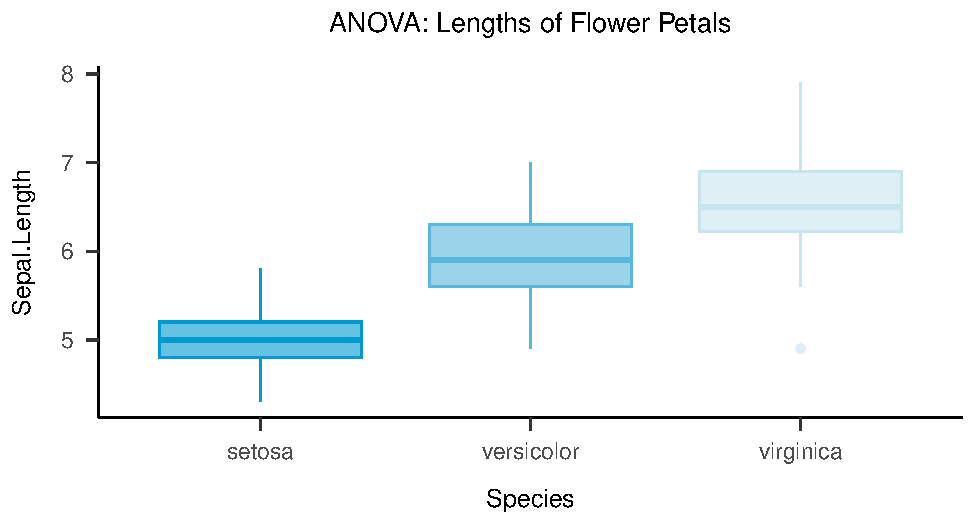
\includegraphics{_main_files/figure-html/unnamed-chunk-54-1.pdf}

\subsection{Pre-Requisites}\label{pre-requisites}

\begin{itemize}
\tightlist
\item
  Load the seminar data using \texttt{seminar\ \textless{}-\ readRDS("./data/seminar\_data.Rds")}

  \begin{itemize}
  \tightlist
  \item
    Please make sure you are using the R dataset from the
    zip folder in ILIAS, not the original csv file we first used!
  \end{itemize}
\item
  Add a ``dummy variable'' (only two possible values 0 and 1)
  for believing in a soul, where 1 means \emph{yes} and 0 means \emph{no or unsure}

  \begin{itemize}
  \tightlist
  \item
    \texttt{seminar\$soul\_dummy\ \textless{}-}
    \texttt{ifelse(seminar\$v11\_soul\ ==\ "yes",\ 1,\ 0)}
  \end{itemize}
\end{itemize}

\section{\texorpdfstring{\(\chi^2\)}{\textbackslash chi\^{}2}}\label{chi2}

\begin{itemize}
\tightlist
\item
  \(\chi^2\) Test for Independence: Determines if there is an association between \textbf{two categorical variables} in a contingency table

  \begin{itemize}
  \tightlist
  \item
    compares the observed frequencies in each category of a contingency table to the frequencies expected if the variables were independent
  \end{itemize}
\end{itemize}

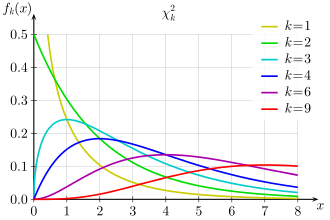
\includegraphics{./img/chidist.png}k

\subsection{Calculation:}\label{calculation}

\begin{itemize}
\item
  \[\chi^2 = \sum \frac{(O_i - E_i)^2}{E_i}\]
\item
  \(O_i\) is the observed frequency in each category
\item
  \(E_i\) is the expected frequency in each category, calculated as: \[E_i = \frac{(row \ total) \times (column \ total)}{grand \ total}\]
\item
  Example: Believing in the soul by gender
\item
\begin{verbatim}
#        
#          0  1 Sum
#   man    1  1   2
#   woman  6  5  11
#   Sum    7  6  13
\end{verbatim}
\end{itemize}

\subsection{How to in R}\label{how-to-in-r}

\begin{itemize}
\item
  The \texttt{chisq.test()} function only needs (categorical!) \emph{x, y} as input

  \begin{itemize}
  \tightlist
  \item
    Especially with a small sample, we can add the parameter \emph{simulate.p.value = T}, which bootstraps the analysis 2000 times
  \end{itemize}
\item
\begin{Shaded}
\begin{Highlighting}[]
\FunctionTok{chisq.test}\NormalTok{(seminar}\SpecialCharTok{$}\NormalTok{v01\_gender, seminar}\SpecialCharTok{$}\NormalTok{soul\_dummy, }\AttributeTok{simulate.p.value =}\NormalTok{ T)}
\CommentTok{\# }
\CommentTok{\#     Pearson\textquotesingle{}s Chi{-}squared test with simulated p{-}value (based on 2000 replicates)}
\CommentTok{\# }
\CommentTok{\# data:  seminar$v01\_gender and seminar$soul\_dummy}
\CommentTok{\# X{-}squared = 0.014069, df = NA, p{-}value = 1}
\end{Highlighting}
\end{Shaded}
\end{itemize}

\subsection{\texorpdfstring{Exercise }{Exercise  }}\label{exercise-3}

We want to explore whether \textbf{belief in the soul (dummy)} is associated with \textbf{music preference}.

Calculate a simple chisq.test and interpret the results.

\subsection{\texorpdfstring{Solution }{Solution  }}\label{solution-2}

\begin{Shaded}
\begin{Highlighting}[]
\FunctionTok{chisq.test}\NormalTok{(seminar}\SpecialCharTok{$}\NormalTok{v07\_genre, seminar}\SpecialCharTok{$}\NormalTok{soul\_dummy)}
\CommentTok{\# Warning in chisq.test(seminar$v07\_genre, seminar$soul\_dummy): Chi{-}squared approximation may be incorrect}
\CommentTok{\# }
\CommentTok{\#   Pearson\textquotesingle{}s Chi{-}squared test}
\CommentTok{\# }
\CommentTok{\# data:  seminar$v07\_genre and seminar$soul\_dummy}
\CommentTok{\# X{-}squared = 2.1357, df = 2, p{-}value = 0.3437}
\FunctionTok{addmargins}\NormalTok{(}\FunctionTok{table}\NormalTok{(seminar}\SpecialCharTok{$}\NormalTok{v07\_genre, seminar}\SpecialCharTok{$}\NormalTok{soul\_dummy))}
\CommentTok{\#         }
\CommentTok{\#           0  1 Sum}
\CommentTok{\#   pop     2  3   5}
\CommentTok{\#   rock    3  3   6}
\CommentTok{\#   techno  2  0   2}
\CommentTok{\#   Sum     7  6  13}
\end{Highlighting}
\end{Shaded}

\begin{itemize}
\tightlist
\item
  Interpretation?
\end{itemize}

\section{t-Test}\label{t-test}

\begin{itemize}
\item
  There are 3 broad categories of t-test:
\item
  \textbf{one-sample} t-test:

  \begin{itemize}
  \tightlist
  \item
    Test one sample against a known mean value
  \end{itemize}
\item
  \textbf{two-sample} t-test (independent):

  \begin{itemize}
  \tightlist
  \item
    Test two sample-means against each other (independent samples)
  \end{itemize}
\item
  \textbf{paired two-sample} t-test:

  \begin{itemize}
  \tightlist
  \item
    Test two dependent sample-means against each other (e.g.~repeated measures)
  \end{itemize}
\end{itemize}

\subsection{\texorpdfstring{Test statistic \emph{t}}{Test statistic t}}\label{test-statistic-t}

\begin{itemize}
\tightlist
\item
  Test statistic T has a known distribution that depends on the \textbf{degrees of freedom}, calculated as n-1
\item
  Most (probable) T values are around 0

  \begin{itemize}
  \tightlist
  \item
    The further away the T value is from 0, the less likely it is caused by chance alone \(\rightarrow\) \emph{significance}
  \end{itemize}
\end{itemize}

\begin{figure}
\centering
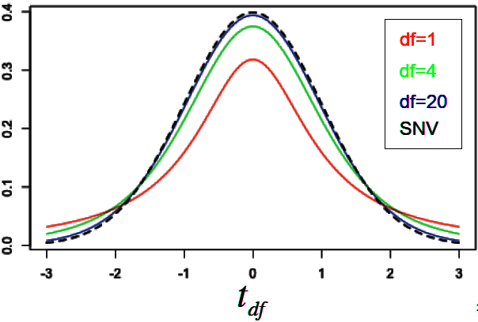
\includegraphics{./img/tdist.png}
\caption{T distribution}
\end{figure}

\subsection{\texorpdfstring{Test statistic \emph{t}}{Test statistic t}}\label{test-statistic-t-1}

\begin{itemize}
\item
  One sample: \[ t = \frac{\bar{X} - \mu}{\frac{s}{\sqrt{n}}} \]
\item
  Two sample: \[t = \frac{\bar{X}_1 - \bar{X}_2}{\sqrt{\frac{s_1^2}{n_1} + \frac{s_2^2}{n_2}}} \]
\end{itemize}

\subsection{How to in R}\label{how-to-in-r-1}

\begin{itemize}
\tightlist
\item
  The basic function is \texttt{t.test()} for any type of t.test
\item
  One sample needs inputs \emph{x, mu} (if x is from a data set you should specify \emph{data})
\item
  Two sample needs either

  \begin{itemize}
  \tightlist
  \item
    \emph{x, y} (if from data set, \emph{data}) or
  \item
    \emph{x \textasciitilde{} group} (if from data set, \emph{data})
  \end{itemize}
\item
  Paired test needs \emph{paired = T}
\item
  One-sided test needs \emph{alternative = `greater'} (assumes first group mean to be larger than second; otherwise ``less'')
\end{itemize}

\subsection{Examples}\label{examples}

\begin{Shaded}
\begin{Highlighting}[]
\CommentTok{\# One sided {-} "greater" assumes that mean(x) is larger than mean(y)}
\FunctionTok{t.test}\NormalTok{(}\AttributeTok{x =} \DecValTok{10}\SpecialCharTok{:}\DecValTok{20}\NormalTok{, }\AttributeTok{y =} \DecValTok{0}\SpecialCharTok{:}\DecValTok{10}\NormalTok{, }\AttributeTok{alternative =} \StringTok{"greater"}\NormalTok{)}
\CommentTok{\# }
\CommentTok{\#   Welch Two Sample t{-}test}
\CommentTok{\# }
\CommentTok{\# data:  10:20 and 0:10}
\CommentTok{\# t = 7.0711, df = 20, p{-}value = 3.713e{-}07}
\CommentTok{\# alternative hypothesis: true difference in means is greater than 0}
\CommentTok{\# 95 percent confidence interval:}
\CommentTok{\#  7.56088     Inf}
\CommentTok{\# sample estimates:}
\CommentTok{\# mean of x mean of y }
\CommentTok{\#        15         5}

\CommentTok{\# Two sided using formula \textasciitilde{} Does seminar motivation differ}
\CommentTok{\# depending on the soul{-}belief of students?}
\FunctionTok{t.test}\NormalTok{(v10\_motivation }\SpecialCharTok{\textasciitilde{}}\NormalTok{ soul\_dummy, }\AttributeTok{data =}\NormalTok{ seminar)}
\CommentTok{\# }
\CommentTok{\#   Welch Two Sample t{-}test}
\CommentTok{\# }
\CommentTok{\# data:  v10\_motivation by soul\_dummy}
\CommentTok{\# t = 0.1625, df = 6.833, p{-}value = 0.8756}
\CommentTok{\# alternative hypothesis: true difference in means between group 0 and group 1 is not equal to 0}
\CommentTok{\# 95 percent confidence interval:}
\CommentTok{\#  {-}31.14063  35.71206}
\CommentTok{\# sample estimates:}
\CommentTok{\# mean in group 0 mean in group 1 }
\CommentTok{\#        68.28571        66.00000}
\end{Highlighting}
\end{Shaded}

\subsection{\texorpdfstring{Exercise }{Exercise }}\label{exercise-4}

We want to test whether the \textbf{gender} stereotype that men are \textbf{more skilled with technology} appears in our seminar sample.

Perform a one-sided two-sample t-test and interpret the results.

Hint: The grouping variable ``v01\_gender'' is sorted alphabetically - so choose the ``alternative'' accordingly!

\subsection{\texorpdfstring{Solution }{Solution }}\label{solution-3}

\begin{Shaded}
\begin{Highlighting}[]
\FunctionTok{t.test}\NormalTok{(v05\_skill\_tech }\SpecialCharTok{\textasciitilde{}}\NormalTok{ v01\_gender, }\AttributeTok{data =}\NormalTok{ seminar, }\AttributeTok{alternative =} \StringTok{"greater"}\NormalTok{)}
\CommentTok{\# }
\CommentTok{\#   Welch Two Sample t{-}test}
\CommentTok{\# }
\CommentTok{\# data:  v05\_skill\_tech by v01\_gender}
\CommentTok{\# t = 0.38715, df = 1.2774, p{-}value = 0.3766}
\CommentTok{\# alternative hypothesis: true difference in means between group man and group woman is greater than 0}
\CommentTok{\# 95 percent confidence interval:}
\CommentTok{\#  {-}109.5565       Inf}
\CommentTok{\# sample estimates:}
\CommentTok{\#   mean in group man mean in group woman }
\CommentTok{\#                46.5                36.0}
\end{Highlighting}
\end{Shaded}

\begin{itemize}
\tightlist
\item
  Interpretation?

  \begin{itemize}
  \tightlist
  \item
    There are no significant gender differences in technological skill.
  \end{itemize}
\end{itemize}

\section{ANOVA}\label{anova}

\begin{figure}
\centering
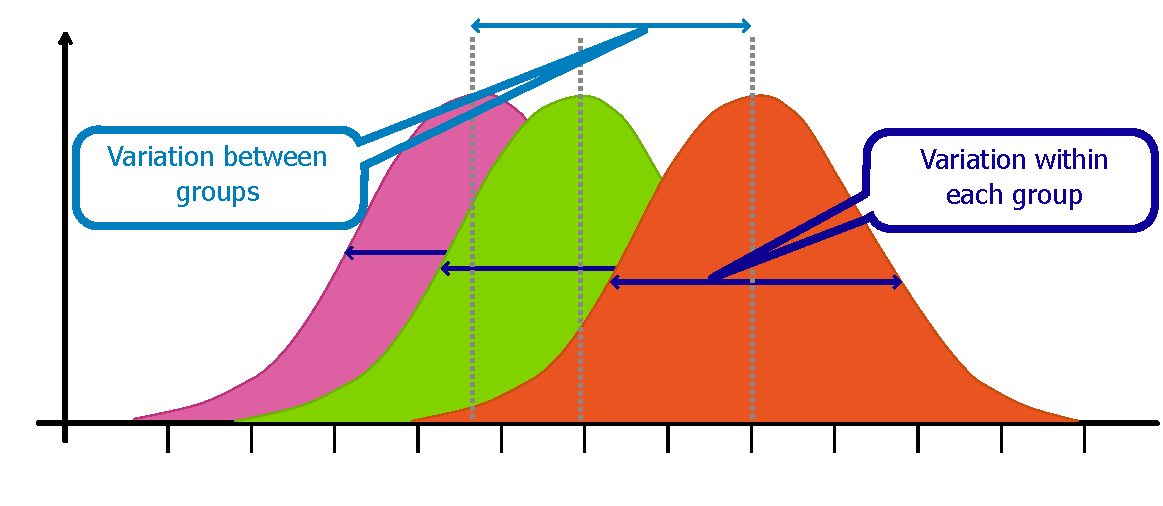
\includegraphics{./img/anova.pdf}
\caption{\label{fig:anovaprince}ANOVA principle}
\end{figure}

\begin{itemize}
\tightlist
\item
  Like a t-test for more than two groups
\item
  Why do we not just calculate several t-tests?

  \begin{itemize}
  \tightlist
  \item
    \(\alpha\) inflation!
  \item
    Significance level of 0.05 means that 1/20 tests will be significant by pure chance, so more tests makes it more likely that we hit that chance and make an alpha error (falsely reject null hypothesis)
  \end{itemize}
\end{itemize}

\subsection{How to - theoretically}\label{how-to---theoretically}

\begin{enumerate}
\def\labelenumi{\arabic{enumi}.}
\tightlist
\item
  Check Assumptions

  \begin{itemize}
  \tightlist
  \item
    Data should be normally distribution \& variance in groups should be similar (homogeneous)
  \end{itemize}
\item
  Sum of Squares: Sum of Squares total, within \& between (\emph{R does this for us})

  \begin{itemize}
  \tightlist
  \item
    F-fraction as the measure of variance explained by the grouping variable in comparison to other variability in the dependent variable
  \end{itemize}
\item
  Interpretation and post-hoc tests

  \begin{itemize}
  \tightlist
  \item
    If there are any significant differences at all, we can use pairwise t-tests (with alpha correction!)
  \end{itemize}
\end{enumerate}

\subsection*{\texorpdfstring{Example: Music genre and loudness }{Example: Music genre and loudness }}\label{example-music-genre-and-loudness}
\addcontentsline{toc}{subsection}{Example: Music genre and loudness }

\subsubsection*{1. Check assumptions}\label{check-assumptions}
\addcontentsline{toc}{subsubsection}{1. Check assumptions}

\begin{itemize}
\item
  Check for Homogeneity of Variance with the Levene Test
\item
\begin{Shaded}
\begin{Highlighting}[]
\CommentTok{\# Make sure the package "car" is installed first! If not, install.packages("car")}
\CommentTok{\# as.factor() forces R to recognize our group as such!}
\NormalTok{car}\SpecialCharTok{::}\FunctionTok{leveneTest}\NormalTok{(v08\_loudness }\SpecialCharTok{\textasciitilde{}} \FunctionTok{as.factor}\NormalTok{(v07\_genre), }\AttributeTok{data =}\NormalTok{ seminar, }\AttributeTok{center =}\NormalTok{ mean)}
\CommentTok{\# Levene\textquotesingle{}s Test for Homogeneity of Variance (center = mean)}
\CommentTok{\#       Df F value Pr(\textgreater{}F)}
\CommentTok{\# group  2  0.1729 0.8437}
\CommentTok{\#       10}
\end{Highlighting}
\end{Shaded}
\item
  Interpretation?

  \begin{itemize}
  \tightlist
  \item
    p value \textless{} 0.05 would indicate significant differences in variance between the group, so we want it to be \textgreater{} 0.05
  \item
    Assumption met!
  \end{itemize}
\end{itemize}

\subsubsection*{2. Define the overall model}\label{define-the-overall-model}
\addcontentsline{toc}{subsubsection}{2. Define the overall model}

\begin{Shaded}
\begin{Highlighting}[]
\NormalTok{model }\OtherTok{\textless{}{-}} \FunctionTok{aov}\NormalTok{(v08\_loudness }\SpecialCharTok{\textasciitilde{}} \FunctionTok{as.factor}\NormalTok{(v07\_genre), }\AttributeTok{data =}\NormalTok{ seminar)}
\FunctionTok{summary}\NormalTok{(model) }\CommentTok{\# "Pr(\textgreater{}F)" is the p{-}value}
\CommentTok{\#                      Df Sum Sq Mean Sq F value Pr(\textgreater{}F)}
\CommentTok{\# as.factor(v07\_genre)  2  618.9   309.4   2.562  0.126}
\CommentTok{\# Residuals            10 1208.0   120.8}
\end{Highlighting}
\end{Shaded}

\begin{itemize}
\tightlist
\item
  Interpretation?

  \begin{itemize}
  \tightlist
  \item
    Not significant (likely due to small sample size)
  \item
    usually we would stop here then, but we will look at the post hoc tests anyway ;)
  \end{itemize}
\end{itemize}

\subsubsection*{3. Post Hoc Test}\label{post-hoc-test}
\addcontentsline{toc}{subsubsection}{3. Post Hoc Test}

\begin{Shaded}
\begin{Highlighting}[]
\FunctionTok{TukeyHSD}\NormalTok{(model)}
\CommentTok{\#   Tukey multiple comparisons of means}
\CommentTok{\#     95\% family{-}wise confidence level}
\CommentTok{\# }
\CommentTok{\# Fit: aov(formula = v08\_loudness \textasciitilde{} as.factor(v07\_genre), data = seminar)}
\CommentTok{\# }
\CommentTok{\# $\textasciigrave{}as.factor(v07\_genre)\textasciigrave{}}
\CommentTok{\#                  diff        lwr      upr     p adj}
\CommentTok{\# rock{-}pop    12.566667  {-}5.677791 30.81112 0.1922467}
\CommentTok{\# techno{-}pop  17.400000  {-}7.808341 42.60834 0.1911143}
\CommentTok{\# techno{-}rock  4.833333 {-}19.767489 29.43416 0.8544384}
\end{Highlighting}
\end{Shaded}

\begin{itemize}
\tightlist
\item
  Interpretation?

  \begin{itemize}
  \tightlist
  \item
    There are no significant pairwise differences in our (small) sample.
  \item
    But we can simulate a larger sample (for fun)
  \end{itemize}
\end{itemize}

\subsection{Addendum for demonstration only: Bootstrapped Data for larger sample size}\label{addendum-for-demonstration-only-bootstrapped-data-for-larger-sample-size}

\begin{Shaded}
\begin{Highlighting}[]
\NormalTok{data }\OtherTok{\textless{}{-}} \FunctionTok{data.frame}\NormalTok{()}

\ControlFlowTok{for}\NormalTok{(i }\ControlFlowTok{in} \DecValTok{1}\SpecialCharTok{:}\DecValTok{10}\NormalTok{)\{}
\NormalTok{  boot }\OtherTok{\textless{}{-}}\NormalTok{ seminar[}\FunctionTok{sample}\NormalTok{(}\DecValTok{1}\SpecialCharTok{:}\FunctionTok{nrow}\NormalTok{(seminar), }\FunctionTok{nrow}\NormalTok{(seminar), }\AttributeTok{replace =}\NormalTok{ T), ]}
\NormalTok{  data }\OtherTok{\textless{}{-}} \FunctionTok{rbind}\NormalTok{(data, boot) }\CommentTok{\# create many random samples from our data }
\NormalTok{\}}

\NormalTok{bootstrapped\_model }\OtherTok{\textless{}{-}} \FunctionTok{aov}\NormalTok{(v08\_loudness }\SpecialCharTok{\textasciitilde{}} \FunctionTok{as.factor}\NormalTok{(v07\_genre), }\AttributeTok{data =}\NormalTok{ data)}
\FunctionTok{summary}\NormalTok{(bootstrapped\_model)}
\CommentTok{\#                       Df Sum Sq Mean Sq F value   Pr(\textgreater{}F)    }
\CommentTok{\# as.factor(v07\_genre)   2   7345    3672   47.76 3.42e{-}16 ***}
\CommentTok{\# Residuals            127   9766      77                     }
\CommentTok{\# {-}{-}{-}}
\CommentTok{\# Signif. codes:  0 \textquotesingle{}***\textquotesingle{} 0.001 \textquotesingle{}**\textquotesingle{} 0.01 \textquotesingle{}*\textquotesingle{} 0.05 \textquotesingle{}.\textquotesingle{} 0.1 \textquotesingle{} \textquotesingle{} 1}
\FunctionTok{TukeyHSD}\NormalTok{(bootstrapped\_model)}
\CommentTok{\#   Tukey multiple comparisons of means}
\CommentTok{\#     95\% family{-}wise confidence level}
\CommentTok{\# }
\CommentTok{\# Fit: aov(formula = v08\_loudness \textasciitilde{} as.factor(v07\_genre), data = data)}
\CommentTok{\# }
\CommentTok{\# $\textasciigrave{}as.factor(v07\_genre)\textasciigrave{}}
\CommentTok{\#                  diff       lwr       upr     p adj}
\CommentTok{\# rock{-}pop    14.238278 10.307525 18.169030 0.0000000}
\CommentTok{\# techno{-}pop  17.624242 11.977093 23.271392 0.0000000}
\CommentTok{\# techno{-}rock  3.385965 {-}2.236703  9.008633 0.3295653}
\end{Highlighting}
\end{Shaded}

\section{\texorpdfstring{Reporting with the \texttt{apa} \& \texttt{papaja} packages}{Reporting with the apa \& papaja packages}}\label{reporting-with-the-apa-papaja-packages}

\begin{itemize}
\tightlist
\item
  You know the \texttt{papaja} package already for \texttt{theme\_apa()} in data visualization
\item
  The package also has many wrapper functions to make reporting in R \& R Markdown a lot easier

  \begin{itemize}
  \tightlist
  \item
    ``apa\_print()''
  \item
    Chi\(^2\) Test reporting cannot be achieved with this, so we use apa::chisq\_apa() for that
  \end{itemize}
\end{itemize}

\subsection{Usage}\label{usage}

\begin{Shaded}
\begin{Highlighting}[]
\CommentTok{\# Chi (add format = "rmarkdown" if needed)}
\NormalTok{apa}\SpecialCharTok{::}\FunctionTok{chisq\_apa}\NormalTok{(}\FunctionTok{chisq.test}\NormalTok{(seminar}\SpecialCharTok{$}\NormalTok{v07\_genre, seminar}\SpecialCharTok{$}\NormalTok{soul\_dummy))}
\CommentTok{\# Warning in chisq.test(seminar$v07\_genre, seminar$soul\_dummy): Chi{-}squared approximation may be incorrect}
\CommentTok{\# chi\^{}2(2) = 2.14, p = .344}

\CommentTok{\# t{-}test}
\NormalTok{papaja}\SpecialCharTok{::}\FunctionTok{apa\_print}\NormalTok{(}\FunctionTok{t.test}\NormalTok{(v05\_skill\_tech }\SpecialCharTok{\textasciitilde{}}\NormalTok{ v01\_gender, }\AttributeTok{data =}\NormalTok{ seminar, }\AttributeTok{alternative =} \StringTok{"greater"}\NormalTok{))}\SpecialCharTok{$}\NormalTok{full\_result}
\CommentTok{\# [1] "$\textbackslash{}\textbackslash{}Delta M = 10.50$, 95\textbackslash{}\textbackslash{}\% CI $[{-}109.56, \textbackslash{}\textbackslash{}infty]$, $t(1.28) = 0.39$, $p = .377$"}

\CommentTok{\# ANOVA}
\NormalTok{papaja}\SpecialCharTok{::}\FunctionTok{apa\_print}\NormalTok{(model)}\SpecialCharTok{$}\NormalTok{full\_result }\SpecialCharTok{|\textgreater{}} \FunctionTok{suppressMessages}\NormalTok{()}
\CommentTok{\# $as\_factorv07\_genre}
\CommentTok{\# [1] "$F(2, 10) = 2.56$, $p = .126$, $\textbackslash{}\textbackslash{}hat\{\textbackslash{}\textbackslash{}eta\}\^{}2\_G = .339$, 90\textbackslash{}\textbackslash{}\% CI $[.000, .602]$"}
\CommentTok{\# suppressMessages() is a useful helper function that avoids any messages from the function it is used with. Here it would just tell us "For one{-}way between subjects designs, generalized eta squared is equivalent to eta squared. Returning eta squared.""}
\end{Highlighting}
\end{Shaded}

\subsection{Usage in R Markdown}\label{usage-in-r-markdown}

\begin{itemize}
\item
  This presentation is based on R Markdown, so we can make use of the pretty printing options right here
\item
  By using \texttt{apa\_print(model)\$full\_result}, we can automatically report results inside our documents:
\item
  ``In our sample, ANOVA showed no significant differences between preferred music genre and preferred volume of listening to music (\(F(2, 10) = 2.56\), \(p = .126\), \(\hat{\eta}^2_G = .339\), 90\% CI \([.000, .602]\)). However, bootstrapping with 10 repetitions suggests that this lack of evidence might be due to the small sample size (\(F(2, 127) = 47.76\), \(p < .001\)), which is also supported by the large effect size (\(\hat{\eta}^2_G = .429\), 90\% CI \([.322, .516]\)).''
\end{itemize}

\section*{Wrap-Up \& Further Resources}\label{wrap-up-further-resources-6}
\addcontentsline{toc}{section}{Wrap-Up \& Further Resources}

Chi\(^2\) test measures association between two categorical variables

t Test measures differences between mean values (one sample, two sample, paired)

ANOVA can be thought of as an augmentation of the t test while controlling alpha inflation

Functions: chisq.test(), t.test(), aov()

Always try to imagine/ keep in mind what you might expect and \emph{what the data would be like if that were true}

Read the documentation of each function for more options

\href{https://the-tave.shinyapps.io/Statistics-Picker/}{Statistics Picker}

\href{https://www.statology.org/chi-square-test-of-independence-in-r/}{Chi2-test (Statology)}

\href{https://www.statology.org/two-sample-t-test/}{t-test (Statology)}

\href{https://www.statology.org/interpret-anova-results-in-r/}{ANOVA (Statology)}

\emph{Discovering Statistics Using R} \citep{field2012}

\begin{figure}
\centering
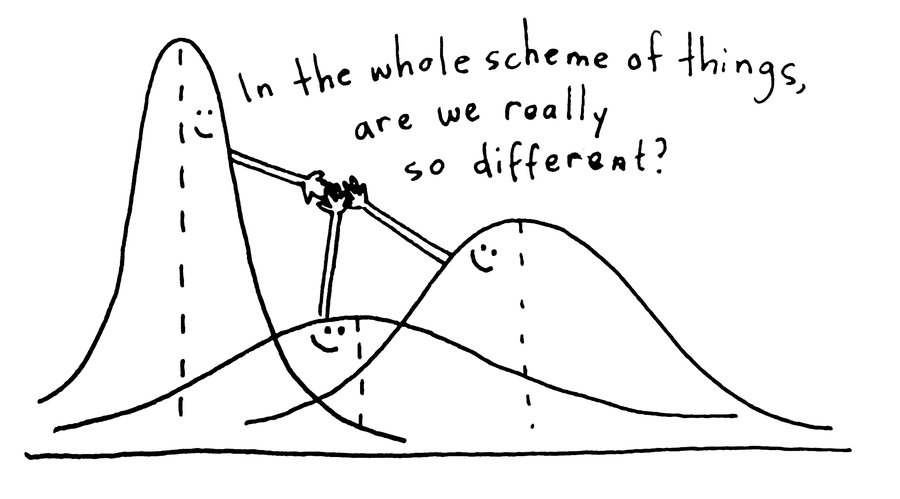
\includegraphics[width=\textwidth,height=2.08333in]{./img/sweet-anova.png}
\caption{Cute ANOVA curves}
\end{figure}

\chapter{Association Statistics}\label{association-statistics}

In this chapter we will look into the correlation and linear regression model in R.

I will assume that you have a basic understanding of what all statistics mentioned in this book are, as they are commonly used among psychologists. However, let's start with a brief statistics re-cap to be on the same page.

Both the correlation - usually reported with Pearson's \emph{r} coefficient - and the regression - also known as (general) linear model - give us measures of \textbf{association}.
The association can be positive (the larger x, the larger y) or negative (the larger x, the smaller y), which is reflected by the sign of the coefficient: \emph{r = 1} would be a perfect positive correlation and \emph{r = -1} would be a perfect negative correlation.

Hopefully, you have heard this one thousand times already, so let me tell you for the thousand and first time: \textbf{Correlation does not imply causation}.
The correlation coefficient r only tells us about the direction and strength of the association and nothing about the causal relation.
However, in the regression model we can check whether Y changes on the basis of X, so we can include assumptions of cause and effect in our model\footnote{A linear model that is ill-defined might still become significant and thus misleading, so your modeling decisions should always be made with a theoretical basis.}

\begin{figure}
\centering
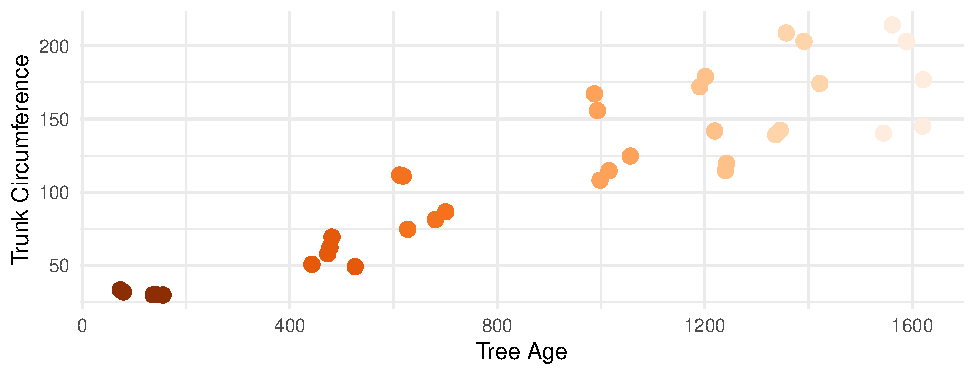
\includegraphics{_main_files/figure-html/tree-age-1.pdf}
\caption{\label{fig:tree-age}Age and circumference of orange trees shown in a scatterplot. We can see that there seems to be a positive relationship between the two measures: The older the tree, the larger the circumference.}
\end{figure}

\subsection{Pre-Requisites}\label{pre-requisites-1}

\begin{itemize}
\tightlist
\item
  Load the seminar data using

  \begin{itemize}
  \tightlist
  \item
    Please make sure you are using the R dataset from the
    zip folder in ILIAS, not the original csv file we first used!
  \end{itemize}
\end{itemize}

\begin{Shaded}
\begin{Highlighting}[]
\NormalTok{seminar }\OtherTok{\textless{}{-}} \FunctionTok{readRDS}\NormalTok{(}\StringTok{"./data/seminar\_data.Rds"}\NormalTok{) }\CommentTok{\# the filepath might need adjustment for you}
\end{Highlighting}
\end{Shaded}

\begin{itemize}
\tightlist
\item
  Some of you were having trouble loading the data - please repeat the different types of data in R and the different commands used to load them! (from week 6)
\item
  \textbf{Who is having trouble opening the slides as HTML?}
\end{itemize}

\section{Correlation}\label{correlation}

\begin{itemize}
\tightlist
\item
  The pearson correlation coefficient r measures association between two numeric variables
\item
  The variables need to

  \begin{itemize}
  \tightlist
  \item
    be \emph{continuous} \& interval-scaled
  \item
    be \emph{normally distributed} \& should have \emph{no outliers}
  \item
    have a \emph{linear relationship}
  \end{itemize}
\item
  Its range is from -1 to 1

  \begin{itemize}
  \tightlist
  \item
    The closer to 0, the weaker the correlation
  \end{itemize}
\end{itemize}

\subsection{Guess the correlation!}\label{guess-the-correlation}

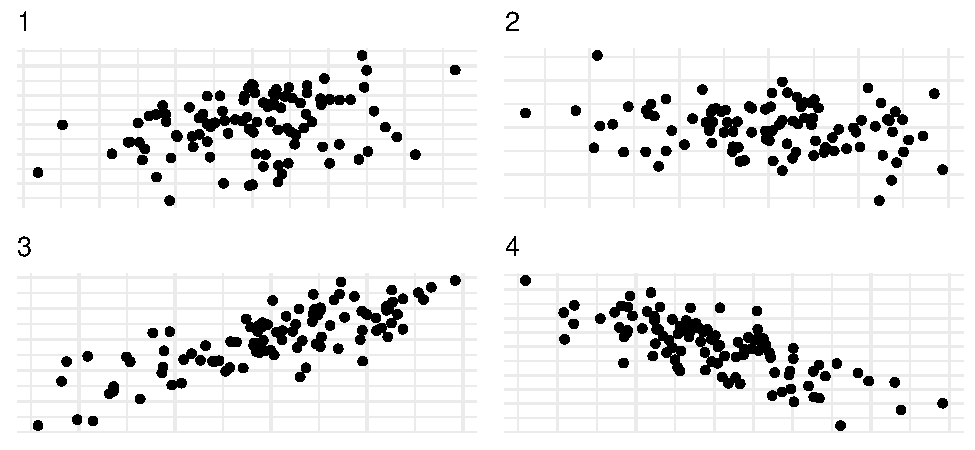
\includegraphics{_main_files/figure-html/corr1-1.pdf}

Solution

r1 = 0.3, r2 = -0.2, r3 = 0.8, r4 = -0.75

\section{Correlation in R}\label{correlation-in-r}

\begin{itemize}
\tightlist
\item
  Two main functions:

  \begin{itemize}
  \tightlist
  \item
    \texttt{cor()} calculates the correlation
  \item
    \texttt{cor.test()} calculates correlation and significance
  \end{itemize}
\item
  As input they both need only an x and a y variable

  \begin{itemize}
  \tightlist
  \item
    You can specify some other aspects of the calculation, such as statistical method (e.g.~``spearman'') or how to deal with missing data
  \end{itemize}
\end{itemize}

\begin{Shaded}
\begin{Highlighting}[]
\NormalTok{x }\OtherTok{\textless{}{-}} \DecValTok{1}\SpecialCharTok{:}\DecValTok{10} 
\NormalTok{y }\OtherTok{\textless{}{-}} \FunctionTok{sample}\NormalTok{(x, }\DecValTok{10}\NormalTok{)}
\FunctionTok{cor}\NormalTok{(x, y)}
\CommentTok{\# [1] {-}0.3333333}
\FunctionTok{cor.test}\NormalTok{(x, y)}
\CommentTok{\# }
\CommentTok{\#   Pearson\textquotesingle{}s product{-}moment correlation}
\CommentTok{\# }
\CommentTok{\# data:  x and y}
\CommentTok{\# t = {-}1, df = 8, p{-}value = 0.3466}
\CommentTok{\# alternative hypothesis: true correlation is not equal to 0}
\CommentTok{\# 95 percent confidence interval:}
\CommentTok{\#  {-}0.7959163  0.3749953}
\CommentTok{\# sample estimates:}
\CommentTok{\#        cor }
\CommentTok{\# {-}0.3333333}
\end{Highlighting}
\end{Shaded}

\subsection{Handling missing data}\label{handling-missing-data}

\begin{itemize}
\item
  Many functions have an option for missing data or \texttt{NA}s

  \begin{itemize}
  \tightlist
  \item
    You can often add the argument \texttt{na.rm\ =\ TRUE} to a function for ``NA remove''
  \end{itemize}
\item
  In the \texttt{cor()} function, we define to only use complete observations
\item
\begin{Shaded}
\begin{Highlighting}[]
\NormalTok{k }\OtherTok{\textless{}{-}} \FunctionTok{c}\NormalTok{(}\DecValTok{1}\NormalTok{, }\DecValTok{2}\NormalTok{, }\DecValTok{3}\NormalTok{, }\DecValTok{4}\NormalTok{, }\DecValTok{5}\NormalTok{)}
\NormalTok{m }\OtherTok{\textless{}{-}} \FunctionTok{c}\NormalTok{(}\DecValTok{1}\NormalTok{, }\DecValTok{3}\NormalTok{, }\DecValTok{2}\NormalTok{, }\DecValTok{5}\NormalTok{, }\ConstantTok{NA}\NormalTok{) }\CommentTok{\# same length but 1 data point is missing}
\FunctionTok{cor}\NormalTok{(k, m)}
\CommentTok{\# [1] NA}
\end{Highlighting}
\end{Shaded}
\item
  With \texttt{use\ =\ "complete.obs"} we define to only use pairs of observations that are not missing
\item
\begin{Shaded}
\begin{Highlighting}[]
\FunctionTok{cor}\NormalTok{(k, m, }\AttributeTok{use =} \StringTok{"complete.obs"}\NormalTok{)}
\CommentTok{\# [1] 0.8315218}
\end{Highlighting}
\end{Shaded}
\item
\begin{Shaded}
\begin{Highlighting}[]
\FunctionTok{cor}\NormalTok{(k[}\DecValTok{1}\SpecialCharTok{:}\DecValTok{4}\NormalTok{], m[}\DecValTok{1}\SpecialCharTok{:}\DecValTok{4}\NormalTok{])}
\CommentTok{\# [1] 0.8315218}
\end{Highlighting}
\end{Shaded}
\end{itemize}

\subsection{Exercise}\label{exercise-5}

Is technology skill associated with seminar motivation?

Calculate a correlation test using \texttt{cor.test()} to analyze the question.

Try to formulate an interpretation as you would report it in a thesis or paper!

Solution

\begin{Shaded}
\begin{Highlighting}[]
\FunctionTok{cor.test}\NormalTok{(seminar}\SpecialCharTok{$}\NormalTok{v05\_skill\_tech, seminar}\SpecialCharTok{$}\NormalTok{v10\_motivation)}
\CommentTok{\# }
\CommentTok{\#   Pearson\textquotesingle{}s product{-}moment correlation}
\CommentTok{\# }
\CommentTok{\# data:  seminar$v05\_skill\_tech and seminar$v10\_motivation}
\CommentTok{\# t = 1.386, df = 11, p{-}value = 0.1932}
\CommentTok{\# alternative hypothesis: true correlation is not equal to 0}
\CommentTok{\# 95 percent confidence interval:}
\CommentTok{\#  {-}0.2100186  0.7724602}
\CommentTok{\# sample estimates:}
\CommentTok{\#       cor }
\CommentTok{\# 0.3855856}
\end{Highlighting}
\end{Shaded}

``With r = 0.386 there is a positive association of moderate strength between previous technological skill and motivation for the seminaR. This association is not significant (p = 0.193), likely due to the small sample size.''

\subsection{Quiz}\label{quiz}

Look at our seminar dataset by entering \texttt{str(seminar)} in the console.
Which of these correlations would work?
Choose ``TRUE'' if you think the correlation would work and ``FALSE'' if you think it would not.
You can look at the explanation for those that would not work below!

\begin{enumerate}
\def\labelenumi{\arabic{enumi}.}
\tightlist
\item
  \texttt{cor(seminar\$v02\_age,\ seminar\$v04\_bodyheight} TRUE / FALSE
\item
  \texttt{cor(seminar\$v02\_age,\ seminar\$v08\_loudness)} TRUE / FALSE
\item
  \texttt{cor(seminar\$v08\_loudness,\ seminar\$v06\_loc)}TRUE / FALSE
\end{enumerate}

Explanation

\begin{enumerate}
\def\labelenumi{\arabic{enumi}.}
\tightlist
\item
  There is a closing bracket missing
\item
  The variable \emph{v06\_loc} has numbers, but they are recognized as characters!
\end{enumerate}

\section{Linear Regression}\label{linear-regression}

\begin{itemize}
\tightlist
\item
  Linear regression also works on numerical, normally distributed data
\item
  We assume an association, and regression can help to look for causation

  \begin{itemize}
  \tightlist
  \item
    There is one \textbf{dependent variable} y and one \textbf{independent variable} x
  \item
    In multiple linear regression, there can be several x
  \end{itemize}
\item
  Formula: \[ y = \beta_0 + \beta x + \epsilon \]
\item
  What we are essentially doing is building a model for our data and checking how well it actually fits!
\end{itemize}

\subsection{Build the model}\label{build-the-model}

\begin{itemize}
\tightlist
\item
  The R function for regression analysis is \texttt{lm()} for \emph{linear model}
\item
  It needs a ``formula'' as input - similar to the formula in the \texttt{t.test()}, we need the \textasciitilde{}

  \begin{itemize}
  \tightlist
  \item
    Read Y \textasciitilde{} X as ``Y on the basis of/ given X''
  \item
    Our dependent variable Y goes first and our independent variable(s) go after the \textasciitilde{}
  \end{itemize}
\item
  If the variables come from a data set, we need to specify data as well
\end{itemize}

\subsection{Visual Inspection}\label{visual-inspection}

\begin{Shaded}
\begin{Highlighting}[]
\FunctionTok{ggplot}\NormalTok{(Orange, }\FunctionTok{aes}\NormalTok{(}\AttributeTok{x =}\NormalTok{ age, }\AttributeTok{y =}\NormalTok{ circumference, }\AttributeTok{color =}\NormalTok{ age)) }\SpecialCharTok{+} \FunctionTok{geom\_jitter}\NormalTok{(}\AttributeTok{size =} \DecValTok{3}\NormalTok{) }\SpecialCharTok{+}
  \FunctionTok{geom\_smooth}\NormalTok{(}\AttributeTok{method =} \StringTok{"lm"}\NormalTok{, }\AttributeTok{se=}\ConstantTok{FALSE}\NormalTok{, }\AttributeTok{color=}\StringTok{"lightgray"}\NormalTok{, }
              \AttributeTok{linewidth =}\NormalTok{ .}\DecValTok{7}\NormalTok{, }\AttributeTok{formula =}\NormalTok{ y }\SpecialCharTok{\textasciitilde{}}\NormalTok{ x) }\SpecialCharTok{+} 
  \FunctionTok{theme\_minimal}\NormalTok{() }\SpecialCharTok{+} 
  \FunctionTok{labs}\NormalTok{(}\AttributeTok{x =} \StringTok{"Tree Age"}\NormalTok{, }\AttributeTok{y =} \StringTok{"Trunk Circumference"}\NormalTok{, }\AttributeTok{title =} \StringTok{"Do trees get thicker with age?"}\NormalTok{) }\SpecialCharTok{+} 
  \FunctionTok{scale\_color\_distiller}\NormalTok{(}\AttributeTok{palette =} \DecValTok{7}\NormalTok{) }\SpecialCharTok{+} 
  \FunctionTok{theme}\NormalTok{(}\AttributeTok{legend.position =} \StringTok{"none"}\NormalTok{)}
\end{Highlighting}
\end{Shaded}

\begin{figure}
\centering
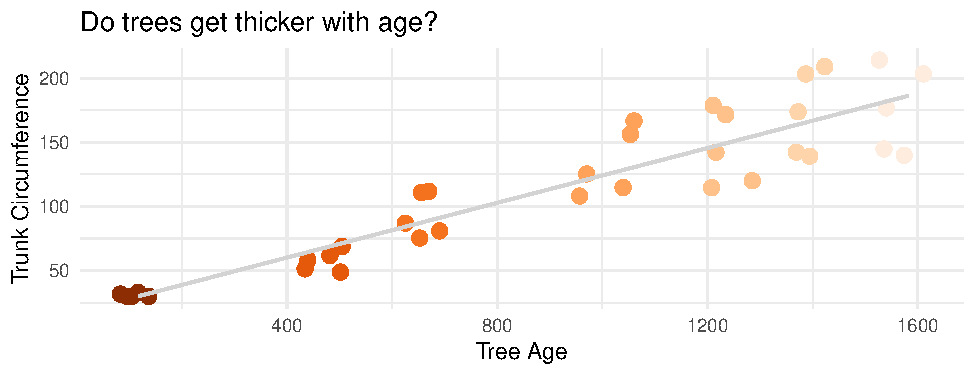
\includegraphics{_main_files/figure-html/tree-age-elaborate-1.pdf}
\caption{\label{fig:tree-age-elaborate}Scatterplot of orange tree age and cirumference from before with the regression line added. Notice that the variable which is used as the independent X (age) is plotted on the X axis for intuitive reading of the plot.}
\end{figure}

What could be problematic here?

\begin{itemize}
\tightlist
\item
  \begin{enumerate}
  \def\labelenumi{(\Alph{enumi})}
  \tightlist
  \item
    homoscedasticity\\
  \end{enumerate}
\item
  \begin{enumerate}
  \def\labelenumi{(\Alph{enumi})}
  \setcounter{enumi}{1}
  \tightlist
  \item
    multicollinearity\\
  \end{enumerate}
\item
  \begin{enumerate}
  \def\labelenumi{(\Alph{enumi})}
  \setcounter{enumi}{2}
  \tightlist
  \item
    heteroscadasticity\\
  \end{enumerate}
\item
  \begin{enumerate}
  \def\labelenumi{(\Alph{enumi})}
  \setcounter{enumi}{3}
  \tightlist
  \item
    oranges
  \end{enumerate}
\end{itemize}

\subsection{Build the model}\label{build-the-model-1}

\subsubsection{Do trees get thicker with age?}\label{do-trees-get-thicker-with-age}

\begin{Shaded}
\begin{Highlighting}[]
\NormalTok{Treelm }\OtherTok{\textless{}{-}} \FunctionTok{lm}\NormalTok{(}\AttributeTok{formula =}\NormalTok{ circumference }\SpecialCharTok{\textasciitilde{}}\NormalTok{ age, }\AttributeTok{data =}\NormalTok{ Orange)}
\NormalTok{Treelm}
\CommentTok{\# }
\CommentTok{\# Call:}
\CommentTok{\# lm(formula = circumference \textasciitilde{} age, data = Orange)}
\CommentTok{\# }
\CommentTok{\# Coefficients:}
\CommentTok{\# (Intercept)          age  }
\CommentTok{\#     17.3997       0.1068}
\end{Highlighting}
\end{Shaded}

\begin{itemize}
\tightlist
\item
  The lm alone gives us the mathematical formula
\item
  To look at the statistical results, we need to use another function such as \texttt{print()} or \texttt{summary()}
\end{itemize}

\subsection{Analyze the model}\label{analyze-the-model}

\begin{Shaded}
\begin{Highlighting}[]
\FunctionTok{summary}\NormalTok{(Treelm)}
\CommentTok{\# }
\CommentTok{\# Call:}
\CommentTok{\# lm(formula = circumference \textasciitilde{} age, data = Orange)}
\CommentTok{\# }
\CommentTok{\# Residuals:}
\CommentTok{\#     Min      1Q  Median      3Q     Max }
\CommentTok{\# {-}46.310 {-}14.946  {-}0.076  19.697  45.111 }
\CommentTok{\# }
\CommentTok{\# Coefficients:}
\CommentTok{\#              Estimate Std. Error t value Pr(\textgreater{}|t|)    }
\CommentTok{\# (Intercept) 17.399650   8.622660   2.018   0.0518 .  }
\CommentTok{\# age          0.106770   0.008277  12.900 1.93e{-}14 ***}
\CommentTok{\# {-}{-}{-}}
\CommentTok{\# Signif. codes:  0 \textquotesingle{}***\textquotesingle{} 0.001 \textquotesingle{}**\textquotesingle{} 0.01 \textquotesingle{}*\textquotesingle{} 0.05 \textquotesingle{}.\textquotesingle{} 0.1 \textquotesingle{} \textquotesingle{} 1}
\CommentTok{\# }
\CommentTok{\# Residual standard error: 23.74 on 33 degrees of freedom}
\CommentTok{\# Multiple R{-}squared:  0.8345,  Adjusted R{-}squared:  0.8295 }
\CommentTok{\# F{-}statistic: 166.4 on 1 and 33 DF,  p{-}value: 1.931e{-}14}
\end{Highlighting}
\end{Shaded}

\begin{itemize}
\tightlist
\item
  Interpretation?

  \begin{itemize}
  \tightlist
  \item
    Trees get larger circumferences the older they are, but this might be modulated by their Species, environment or other factors
  \end{itemize}
\end{itemize}

\subsection{\texorpdfstring{Exercise }{Exercise  }}\label{exercise-6}

Does the age of a person have an influence on how long they took to complete the seminar survey (session length)?

Use the \texttt{lm()} function and report the significance level of the predictor as well as the model equation.

Solution (code)

\begin{Shaded}
\begin{Highlighting}[]
\NormalTok{age\_sess }\OtherTok{\textless{}{-}} \FunctionTok{lm}\NormalTok{(session\_length }\SpecialCharTok{\textasciitilde{}}\NormalTok{ v02\_age, }\AttributeTok{data =}\NormalTok{ seminar)}
\FunctionTok{summary}\NormalTok{(age\_sess)}
\CommentTok{\# }
\CommentTok{\# Call:}
\CommentTok{\# lm(formula = session\_length \textasciitilde{} v02\_age, data = seminar)}
\CommentTok{\# }
\CommentTok{\# Residuals:}
\CommentTok{\#     Min      1Q  Median      3Q     Max }
\CommentTok{\# {-}34.978  {-}5.605   1.209  13.395  36.141 }
\CommentTok{\# }
\CommentTok{\# Coefficients:}
\CommentTok{\#             Estimate Std. Error t value Pr(\textgreater{}|t|)  }
\CommentTok{\# (Intercept)  182.706     61.517   2.970   0.0127 *}
\CommentTok{\# v02\_age       {-}4.186      2.689  {-}1.557   0.1478  }
\CommentTok{\# {-}{-}{-}}
\CommentTok{\# Signif. codes:  0 \textquotesingle{}***\textquotesingle{} 0.001 \textquotesingle{}**\textquotesingle{} 0.01 \textquotesingle{}*\textquotesingle{} 0.05 \textquotesingle{}.\textquotesingle{} 0.1 \textquotesingle{} \textquotesingle{} 1}
\CommentTok{\# }
\CommentTok{\# Residual standard error: 21.23 on 11 degrees of freedom}
\CommentTok{\# Multiple R{-}squared:  0.1805,  Adjusted R{-}squared:  0.106 }
\CommentTok{\# F{-}statistic: 2.423 on 1 and 11 DF,  p{-}value: 0.1478}
\end{Highlighting}
\end{Shaded}

Solution (interpretation)

``The age of a person does not significantly predict the time it took them to complete the survey (p = .148). The model equation is 182.7 -4.19X with age explaining about 18\% of the variance in session length for the survey.''

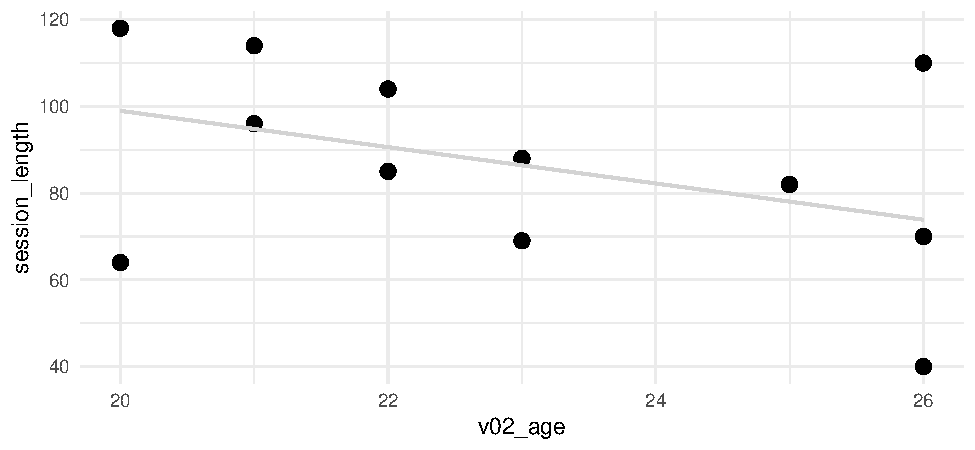
\includegraphics{_main_files/figure-html/age-sess-1.pdf}

\subsection{A word to the wise}\label{a-word-to-the-wise}

\begin{itemize}
\tightlist
\item
  There is also a function called \texttt{glm()} for general linear model
\item
  In the cases I showed you, both perform the same tasks
\item
  The \texttt{glm()} can also handle other more advanced statistical analyses, including logistic regression
\item
  However, the \texttt{lm()} function will output the coefficient of determination \(R^2\)

  \begin{itemize}
  \tightlist
  \item
    It tell us the proportion of the variation in the dependent variable that is predictable from the independent variable(s)
  \item
    We \emph{could} also calculate it by hand using the \texttt{cor()} function and squaring the result
  \end{itemize}
\end{itemize}

\section{ANOVA Exercise}\label{anova-exercise}

Reminder: There are generally 3 steps to an ANOVA

\begin{Shaded}
\begin{Highlighting}[]
\NormalTok{car}\SpecialCharTok{::}\FunctionTok{leveneTest}\NormalTok{(v08\_loudness }\SpecialCharTok{\textasciitilde{}}\NormalTok{ v11\_soul, }\AttributeTok{data =}\NormalTok{ seminar) }\CommentTok{\# 1.}
\NormalTok{model }\OtherTok{\textless{}{-}} \FunctionTok{aov}\NormalTok{(v08\_loudness }\SpecialCharTok{\textasciitilde{}}\NormalTok{ v11\_soul, }\AttributeTok{data =}\NormalTok{ seminar) }\CommentTok{\# 2.}
\FunctionTok{summary}\NormalTok{(model)}
\FunctionTok{TukeyHSD}\NormalTok{(model) }\CommentTok{\# 3.}
\end{Highlighting}
\end{Shaded}

\begin{enumerate}
\def\labelenumi{\arabic{enumi}.}
\tightlist
\item
  Check assumptions with Levene Test
\item
  Build the model to perform an omnibus ANOVA
\item
  Perform post-hoc tests to check pairwise differences (usually only if the omnibus ANOVA is significant)
\end{enumerate}

\subsection{Exercise}\label{exercise-7}

\textbf{Does the preferred music volume depend on someone's soul philosophy?}

Perform an ANOVA on our seminar data to explore the question (v08 \& v12).

Solution omnibus ANOVA

\begin{Shaded}
\begin{Highlighting}[]
\NormalTok{car}\SpecialCharTok{::}\FunctionTok{leveneTest}\NormalTok{(v08\_loudness }\SpecialCharTok{\textasciitilde{}}\NormalTok{ v12\_soul\_phil, }\AttributeTok{data =}\NormalTok{ seminar)}
\CommentTok{\# Warning in leveneTest.default(y = y, group = group, ...): group coerced to factor.}
\CommentTok{\# Levene\textquotesingle{}s Test for Homogeneity of Variance (center = median)}
\CommentTok{\#       Df F value Pr(\textgreater{}F)}
\CommentTok{\# group  2  0.3112 0.7394}
\CommentTok{\#       10}
\NormalTok{model }\OtherTok{\textless{}{-}} \FunctionTok{aov}\NormalTok{(v08\_loudness }\SpecialCharTok{\textasciitilde{}}\NormalTok{ v12\_soul\_phil, }\AttributeTok{data =}\NormalTok{ seminar)}
\FunctionTok{summary}\NormalTok{(model)}
\CommentTok{\#               Df Sum Sq Mean Sq F value  Pr(\textgreater{}F)   }
\CommentTok{\# v12\_soul\_phil  2 1164.8   582.4   8.797 0.00625 **}
\CommentTok{\# Residuals     10  662.1    66.2                   }
\CommentTok{\# {-}{-}{-}}
\CommentTok{\# Signif. codes:  0 \textquotesingle{}***\textquotesingle{} 0.001 \textquotesingle{}**\textquotesingle{} 0.01 \textquotesingle{}*\textquotesingle{} 0.05 \textquotesingle{}.\textquotesingle{} 0.1 \textquotesingle{} \textquotesingle{} 1}
\end{Highlighting}
\end{Shaded}

Look for pairwise differences even if the overall ANOVA does not reach significance.

Solution pairwise comparison

\begin{Shaded}
\begin{Highlighting}[]
\FunctionTok{TukeyHSD}\NormalTok{(model)}
\CommentTok{\#   Tukey multiple comparisons of means}
\CommentTok{\#     95\% family{-}wise confidence level}
\CommentTok{\# }
\CommentTok{\# Fit: aov(formula = v08\_loudness \textasciitilde{} v12\_soul\_phil, data = seminar)}
\CommentTok{\# }
\CommentTok{\# $v12\_soul\_phil}
\CommentTok{\#                      diff        lwr       upr     p adj}
\CommentTok{\# dunno{-}dualism    9.714286  {-}5.678116 25.106687 0.2419042}
\CommentTok{\# monism{-}dualism {-}13.666667 {-}31.879202  4.545868 0.1490289}
\CommentTok{\# monism{-}dunno   {-}23.380952 {-}38.773354 {-}7.988551 0.0049965}
\end{Highlighting}
\end{Shaded}

Choose and create an appropriate visualization for this data!

Solution Data Viz

\begin{Shaded}
\begin{Highlighting}[]
\FunctionTok{ggplot}\NormalTok{(seminar, }\FunctionTok{aes}\NormalTok{(}\AttributeTok{x =}\NormalTok{ v12\_soul\_phil, }\AttributeTok{y =}\NormalTok{ v08\_loudness, }
                    \AttributeTok{color =}\NormalTok{ v12\_soul\_phil, }\AttributeTok{fill =}\NormalTok{ v12\_soul\_phil)) }\SpecialCharTok{+}
  \FunctionTok{geom\_boxplot}\NormalTok{(}\AttributeTok{alpha =}\NormalTok{ .}\DecValTok{7}\NormalTok{) }\SpecialCharTok{+} 
  \FunctionTok{theme\_minimal}\NormalTok{() }\SpecialCharTok{+} 
  \FunctionTok{theme}\NormalTok{(}\AttributeTok{legend.position =} \StringTok{"none"}\NormalTok{) }\SpecialCharTok{+}
  \FunctionTok{labs}\NormalTok{(}\AttributeTok{x =} \StringTok{"Soul Philosophy"}\NormalTok{, }\AttributeTok{y =} \StringTok{"Preferred Volume (arbitrary units)"}\NormalTok{) }\SpecialCharTok{+}
  \FunctionTok{scale\_color\_brewer}\NormalTok{(}\AttributeTok{palette =} \DecValTok{4}\NormalTok{) }\SpecialCharTok{+} \FunctionTok{scale\_fill\_brewer}\NormalTok{(}\AttributeTok{palette =} \DecValTok{4}\NormalTok{)}
\end{Highlighting}
\end{Shaded}

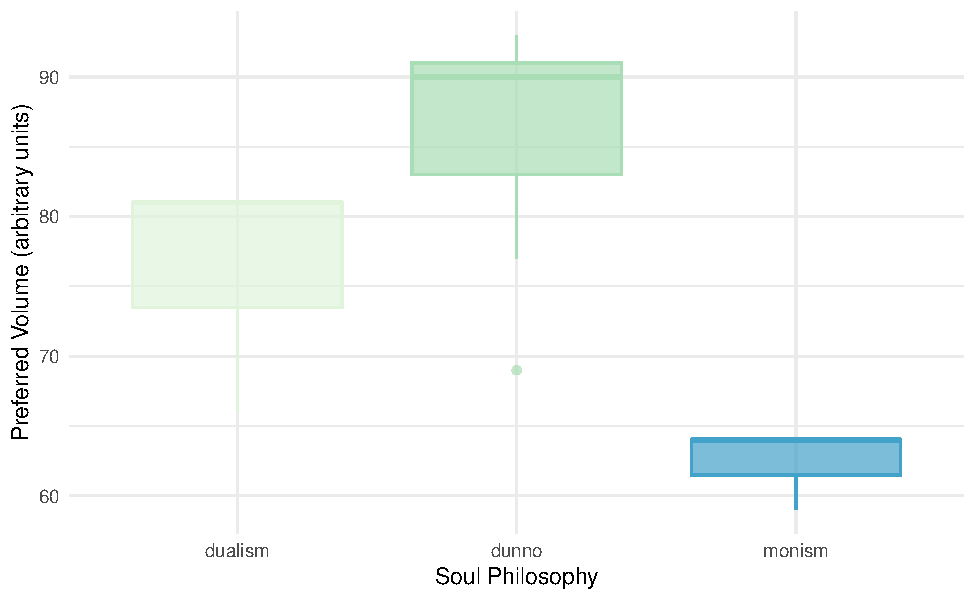
\includegraphics{_main_files/figure-html/unnamed-chunk-71-1.pdf}

\section*{Wrap-Up \& Further Resources}\label{wrap-up-further-resources-7}
\addcontentsline{toc}{section}{Wrap-Up \& Further Resources}

Correlation coefficient \emph{r} can be determined using \texttt{cor(x,y)}

\(R^2\) is the coefficient of determination in a linear model (calculate by hand or in the model formula)

The linear model function \texttt{lm()} is used to build models for linear regression

Problems such as overfitting or heteroscedasticity reduce the interpretability of the model results

\href{https://www.guessthecorrelation.com/}{Guess the Correlation}

\href{https://statisticsbyjim.com/basics/correlation-coefficient-formula/}{Explanation: Correlation}

\href{https://www.datacamp.com/tutorial/linear-regression-R}{Linear Regression in R}

\href{https://www.codecademy.com/learn/learn-linear-regression-in-r/modules/linear-regression-in-r/cheatsheet/}{lm() cheatsheet}

\begin{Shaded}
\begin{Highlighting}[]
\FunctionTok{ggplot}\NormalTok{(Orange, }\FunctionTok{aes}\NormalTok{(}\AttributeTok{x =}\NormalTok{ age, }\AttributeTok{y =}\NormalTok{ circumference, }\AttributeTok{color =}\NormalTok{ Tree)) }\SpecialCharTok{+}
  \FunctionTok{geom\_point}\NormalTok{(}\AttributeTok{size =} \DecValTok{3}\NormalTok{) }\SpecialCharTok{+} \FunctionTok{labs}\NormalTok{(}\AttributeTok{x =} \StringTok{"Tree Age"}\NormalTok{, }\AttributeTok{y =} \StringTok{"Trunk Circumference"}\NormalTok{) }\SpecialCharTok{+}
  \FunctionTok{geom\_line}\NormalTok{(}\FunctionTok{aes}\NormalTok{(}\AttributeTok{color =}\NormalTok{ Tree)) }\SpecialCharTok{+} \FunctionTok{theme\_minimal}\NormalTok{() }\SpecialCharTok{+} \FunctionTok{theme}\NormalTok{(}\AttributeTok{legend.position =} \StringTok{"none"}\NormalTok{)}
\end{Highlighting}
\end{Shaded}

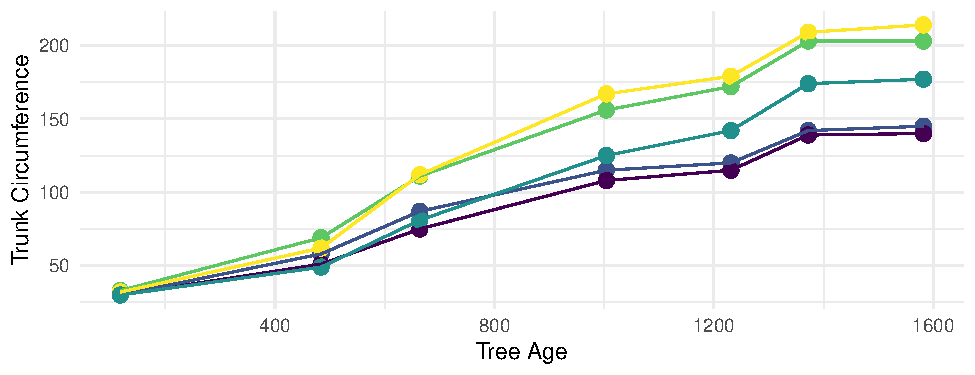
\includegraphics{_main_files/figure-html/orange-pretty-1.pdf}

\part{Reporting in R}\label{part-reporting-in-r}

\chapter{R Markdown}\label{r-markdown}


\includegraphics[width=\textwidth,height=1.04167in]{./img/rmd.png}

In this last part we will learn one of the most nifty features of R, which is being able to create whole documents from the comfort of your R Studio.
Because creating visualizations and statistics in R is great, but we need to able to show and report our work.
Of course, results can be copied and plots can be exported, but the more steps one needs to take, the more prone to error the work becomes. When you write a report with this feature, analyses and plots can be embedded directly into the document.
Basically, R Markdown is a text engine based on \LaTeX that allows you to create documents, presentations, reports and much more.
As I mentioned before, it can be used to write whole theses - an example of which you can see in the screenshot below!

\begin{figure}
\centering
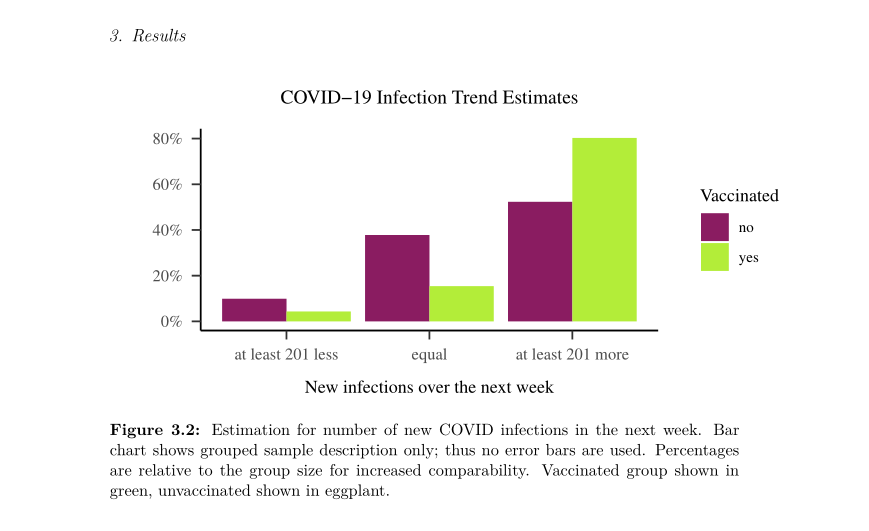
\includegraphics[width=\textwidth,height=2.60417in]{./img/MArmdex.png}
\caption{\emph{\textbf{Example Screenshot of a Thesis written in R Markdown}}}
\end{figure}

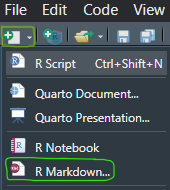
\includegraphics[width=\textwidth,height=1.77083in]{./img/rmd-click.png}

There are many possibilities and luckily, there are also usually templates and guidelines to go along with them.
For your first R Markdown document, you can create a demo Rmd with the ``New File'' menu as shown, or go to File \textgreater{} New File \textgreater{} R Markdown to create a new Rmd document.
Give it a name or keep all the defaults for now.
It will create a document with some demo content.
When you click the ``knit''-button below the main menu, you will need to save the file and it will create the output.
Try to play around with the text and read the demo content - it explains the basic functions!
You can use the document you create now as a sort of cheatsheet and template for what you can do later.

RMarkdown has some basics that need to be learned and might take some getting used to.
It also has many features and powerful tools for layout and styling, so spending the time it takes to learn is a good investment.
By default, RMarkdown can create HTML\footnote{HTML is used in most if not all websites and stands for \emph{hypertext markup language}.} documents.
Don't worry if that sounds like more programming to you - while it is possible to use special \emph{HTML tags} in R Markdown, it is by no means necessary.

You can also create other types of documents, such as a pdf for which you need a special package to render \LaTeX.
The most efficient is usually \texttt{tinytex}, which first needs to be installed as the package itself and afterwards it can run its own installation of everything you need for your reporting:

\begin{Shaded}
\begin{Highlighting}[]
\FunctionTok{install.packages}\NormalTok{(}\StringTok{"tinytex"}\NormalTok{)}
\NormalTok{tinytex}\SpecialCharTok{::}\FunctionTok{install\_tinytex}\NormalTok{()}
\end{Highlighting}
\end{Shaded}

\section{\texorpdfstring{YAML header (\emph{Yet Another Markdown Language})}{YAML header (Yet Another Markdown Language)}}\label{yaml-header-yet-another-markdown-language}

Apart from the document processors that are necessary, R Markdown files also follow a specific structure in order to be recognized as the right type of file.
Every R Markdown document starts with the so-called YAML header, which stands for \emph{Yet Another Markdown Language}.
This defines most of the ``hard facts'' concerning our document, such the output format, e.g.~\texttt{html\_document}, title, subtitle, author, date\ldots{}
We can also define further characteristics, e.g.~\texttt{toc} (table of content) or \texttt{self-contained} (this should be set to true, otherwise R will not copy images etc. and the document will not work properly on other devices).

\begin{quote}
The YAML header needs to be indented in a certain way, otheriwse the commands are not recognized!
\end{quote}

\begin{Shaded}
\begin{Highlighting}[]
\SpecialCharTok{{-}{-}{-}}
\NormalTok{title}\SpecialCharTok{:} \StringTok{"My Title"}
\NormalTok{subtitle}\SpecialCharTok{:} \ErrorTok{|}
    \ErrorTok{|}\NormalTok{ A Super, Very,}
    \SpecialCharTok{|}\NormalTok{ Insanely Long}
    \SpecialCharTok{|}\NormalTok{ Awesome Subtitle}
    \SpecialCharTok{|}\NormalTok{ In Four Lines}
\NormalTok{author}\SpecialCharTok{:} \StringTok{"A Great Author"}
\NormalTok{date}\SpecialCharTok{:} \StringTok{"\textasciigrave{}r Sys.Date()\textasciigrave{}"}
\NormalTok{output}\SpecialCharTok{:} 
\NormalTok{  pdf\_document}\SpecialCharTok{:}
\NormalTok{    toc}\SpecialCharTok{:}\NormalTok{ true}
\NormalTok{    self}\SpecialCharTok{{-}}\NormalTok{containted}\SpecialCharTok{:}\NormalTok{ true}
\SpecialCharTok{{-}{-}{-}}

\CommentTok{\# First Chapter}

\NormalTok{Start text after a blank line}\SpecialCharTok{!} 
\end{Highlighting}
\end{Shaded}

As you can see above, the YAML header is surrounded by three minus signs --- and has quite specific formatting.
Setting values like title and author are similar to assigning strings to variables - they have to be put in quotes.
One exception to this rule can be seen in the subtitle, which starts with a vertical rule \textbar{} - if that is the case, you can define very long text without the quotes and even control the exact format and line break.
Another nifty feature is being able to use inline R Code, to e.g.~insert today's date automatically with ` r Sys.Date()`.

For the output, it is important to stick with this type of indentation, where every setting belonging to the document command is indented further than the document definition.

\begin{quote}
In the YAML header, \texttt{true} and \texttt{false} are not capitalized, unlike in the rest of R!
\end{quote}

\section{Markdown Basics}\label{markdown-basics}

When you have defined the document basics to your liking, it is time to get started on the actual text.
While other text processors offer buttons for text formatting, R Markdown requires this formatting to be included in the text.
Think of Markdown as the back-end of your document and the output as the front-end!

Here is an overview of the most important formatting features:

\begin{itemize}
\tightlist
\item
  \emph{italics} with \_italics\_
\item
  \textbf{bold} with **bold**
\item
  \textbf{\emph{bold and cursive}} with **\_bold and cursive\_**
\item
  Unordered lists are created with -
\item
  Ordered lists with 1., 2. \ldots{}
\end{itemize}

To structure your text, you can set headings with the \# pound sign.
The more pound signs, the smaller the heading (sub-levels).

\# First Heading
\#\# Sub Header 2. level
\#\#\# Sub Header 3. level
\#\#\#\# 4th level
\#\#\#\#\# 5th level
\#\#\#\#\#\# 6th level

Realistically, we \emph{may} want to go down to the 4th level heading, but usually no further.

\subsection*{Tables}\label{tables}
\addcontentsline{toc}{subsection}{Tables}

To create tables, we also need to specify rows and columns with symbols right in the text.
Anything above the line of minus signs is identified as the header and anything below as the table content.
This is a fairly simple way to create automatically formatted, clean tables.

Header 1 \textbar{} Header 2
-----\textbar-----
Great content \textbar{} Fantastic content

Becomes:

\begin{longtable}[]{@{}ll@{}}
\toprule\noalign{}
Header 1 & Header 2 \\
\midrule\noalign{}
\endhead
\bottomrule\noalign{}
\endlastfoot
Great content & Fantastic content \\
\end{longtable}

It is also possible to use inline Code to report statistics, although it may be more efficient for reporting to create tables with \texttt{kable}, which you can read more about \href{https://cran.r-project.org/web/packages/kableExtra/vignettes/awesome_table_in_html.html}{here}.

\section{Special Features}\label{special-features}

\begin{itemize}
\tightlist
\item
  Print mathematical equations
\item
  Show code and its output
\item
  Easily use automatic formatting
\item
  Profit from existing templates
\item
  General rule of thumb: Rmd documents are rendered depending on their output format

  \begin{itemize}
  \tightlist
  \item
    If you plan on creating an html, you can use plain html to make adjustments and use special features.
  \item
    If you create a pdf, they will most likely not work and you should use \LaTeX notation.
  \end{itemize}
\end{itemize}

\subsection{\texorpdfstring{\LaTeX}{}}\label{section}

Especially useful for writing equations:

\begin{itemize}
\tightlist
\item
  \$ \textbackslash{} alpha \$ \(\rightarrow\) \(\alpha\)
\item
  \$ \textbackslash{} beta \$ \(\rightarrow\) \(\beta\)
\item
  \$ R\^{}2 \$ \(\rightarrow\) \(R^2\)
\item
  and, by the way, \$ \textbackslash{} rightarrow \$ becomes \(\rightarrow\)
\item
  and \$ \textbackslash{} LaTeX \$ becomes \LaTeX
\item
  \textbackslash{} newline creates a new line and \textbackslash{} newpage creates a new page
\end{itemize}

\subsection{HTML}\label{html}

Remember these tags should only be used when creating a html document!

\begin{itemize}
\tightlist
\item
  \textless{} br \textgreater{} creates a new line (stands for ``line break'')
\item
  \textless span style=``color: purple;''\textgreater{} This text will appear purple. \textless/span\textgreater{}

  \begin{itemize}
  \tightlist
  \item
    { This text will appear purple. }
  \end{itemize}
\item
  Simple tables can be created with html notation in most documents

  \begin{itemize}
  \tightlist
  \item
    Header 1 \textbar{} Header 2
  \item
    \emph{then a row of - - - \textbar{} - - - to represent the lines}
  \item
    And the content separated \textbar{} into as many columns as defined
  \end{itemize}
\end{itemize}

\section{Including R}\label{including-r}

\begin{itemize}
\tightlist
\item
  Including R code can be achieved by either inserting so-called code chunks or using inline code
\item
  Code chunks are useful if several lines of code need to be evaluated and/ or shown

  \begin{itemize}
  \tightlist
  \item
    There are many options for code chunks
  \end{itemize}
\item
  Inline code is useful if single outputs are to be shown

  \begin{itemize}
  \tightlist
  \item
    E.g. with functions you already know such as \texttt{apa\_print()}
  \end{itemize}
\end{itemize}

\subsection{Code Chunks}\label{code-chunks}

\begin{itemize}
\item
  Code chunks are inserted via the menu Code \textgreater{} Insert Chunk and should look like this:
\item
  ```\{r\}
  \# \emph{code goes here}
  ```
\item
\begin{Shaded}
\begin{Highlighting}[]
\CommentTok{\# code goes here}
\end{Highlighting}
\end{Shaded}
\item
  Or you can use the keyboard shortcut ctrl + alt + i / command + option + i
\end{itemize}

\subsubsection*{Chunk Options}\label{chunk-options}
\addcontentsline{toc}{subsubsection}{Chunk Options}

\begin{itemize}
\item
  Inside the curly brackets, you can specify many different options, for example:

  \begin{itemize}
  \tightlist
  \item
    \texttt{fig.height\ =\ 3} will output a plot to a certain height (3 inches)
  \item
    \texttt{echo\ =\ F} will show code output, but not the code
  \item
    \texttt{eval\ =\ F} will show the code, but not its' output\ldots{}
  \end{itemize}
\item
  eval = F:

\begin{Shaded}
\begin{Highlighting}[]
\FunctionTok{head}\NormalTok{(iris, }\DecValTok{1}\NormalTok{) }
\end{Highlighting}
\end{Shaded}
\item
  echo = F:

\begin{verbatim}
#   Sepal.Length Sepal.Width Petal.Length Petal.Width Species
# 1          5.1         3.5          1.4         0.2  setosa
\end{verbatim}
\end{itemize}

\paragraph*{\texorpdfstring{\texttt{error\ =\ TRUE}}{error = TRUE}}\label{error-true}
\addcontentsline{toc}{paragraph}{\texttt{error\ =\ TRUE}}

\begin{itemize}
\tightlist
\item
  This option allows us to include erroneous code in our script
\item
  It will output the error message just like you would see in your R Studio console
\item
  By default, \texttt{error\ =\ FALSE} which means that your script cannot be rendered with errors in code chunks
\end{itemize}

\begin{Shaded}
\begin{Highlighting}[]
\FunctionTok{mean}\NormalTok{(y)}
\CommentTok{\# [1] 5.5}
\end{Highlighting}
\end{Shaded}

\section*{Wrap-Up \& Further Resources}\label{wrap-up-further-resources-8}
\addcontentsline{toc}{section}{Wrap-Up \& Further Resources}

RMarkdown allows you to create professional documents

You can use it like other text-generating programs (e.g.~MS Word)

Embed plots, code and statistical results directly in your document

Show equations and use other special features

\href{https://www.youtube.com/watch?v=asHhuHRxhvo&ab_channel=EquitableEquations/}{YouTube: What is R Markdown?}

\href{https://wch.github.io/latexsheet/}{LaTeX Cheatsheet}

\href{https://web.stanford.edu/group/csp/cs21/htmlcheatsheet.pdf}{HTML Cheatsheet}

\href{https://bookdown.org/yihui/rmarkdown-cookbook/}{RMarkdown Cookbook}

\href{https://yihui.org/knitr/options/}{RMarkdown Chunk Options}

\href{https://www.youtube.com/watch?v=01KifhHDkFk&ab_channel=EquitableEquations}{YouTube: Presentations with Quarto}

\begin{figure}
\centering

\includegraphics[width=\textwidth,height=5.72917in]{img/shakespeare.jpg}
\caption{Shakespeare writing RMarkdown (AI generated using the \href{https://www.bing.com/images/create}{bing image creator})}
\end{figure}

\chapter{The Power of R \& R Markdown}\label{the-power-of-r-r-markdown}

\begin{figure}
\centering

\includegraphics{./img/papaja.png}
\caption{Happy Papaya Logo}
\end{figure}

\section{Quiz - Rmd specific}\label{quiz---rmd-specific}

\begin{enumerate}
\def\labelenumi{\arabic{enumi}.}
\tightlist
\item
  What do I need to do to make my text \textbf{\emph{look like this}}?

  \begin{itemize}
  \tightlist
  \item
    **\_look like this\_**
  \end{itemize}
\item
  I want to add a subtitle to my document, where might I do that?

  \begin{itemize}
  \tightlist
  \item
    Add `subtitle: ``A great subtitle''\,' to the \textbf{YAML header}
  \end{itemize}
\item
  How do I generate a section header in my document?

  \begin{itemize}
  \tightlist
  \item
    With the pound sign \# Header
  \end{itemize}
\item
  Oh no, my header isn't showing up right! What could have happened?

  \begin{itemize}
  \tightlist
  \item
    There needs to be a space between the \# and the header
  \end{itemize}
\end{enumerate}

\subsection{Quiz - general R}\label{quiz---general-r}

\begin{enumerate}
\def\labelenumi{\arabic{enumi}.}
\item
  What package contains the functions \texttt{select,\ filter\ \&\ mutate}?

  \begin{itemize}
  \tightlist
  \item
    \texttt{dplyr} (or \texttt{tidyverse})
  \end{itemize}
\item
  Assume I have created some R project and I read a file with the following command - what does this tell you about the folder on my computer?

\begin{Shaded}
\begin{Highlighting}[]
\NormalTok{greatdata }\OtherTok{\textless{}{-}}\NormalTok{ readr}\SpecialCharTok{::}\FunctionTok{read\_csv}\NormalTok{(}\AttributeTok{file =} \StringTok{"./data/somefile.CSV"}\NormalTok{)}
\end{Highlighting}
\end{Shaded}

  \begin{itemize}
  \tightlist
  \item
    The folder containing the R project contains a subfolder called ``data'' and in there is a CSV file called ``somefile.csv''.
  \end{itemize}
\end{enumerate}

\subsection{Quiz - general R}\label{quiz---general-r-1}

\begin{enumerate}
\def\labelenumi{\arabic{enumi}.}
\setcounter{enumi}{2}
\tightlist
\item
  I want to load a csv file into R with \texttt{readRDS()}. Why isn't it working?

  \begin{itemize}
  \tightlist
  \item
    The read commands are specific to the file format. readRDS() is for R files, read.csv() or readr::read\_csv() are needed for csv files
  \end{itemize}
\item
  What do you know when you look at the command \texttt{bigfive\$extraversion}?

  \begin{itemize}
  \tightlist
  \item
    There is a data set called \texttt{bigfive} and we're accessing a variable called \texttt{extraversion}
  \end{itemize}
\end{enumerate}

\subsection{Quiz - general R}\label{quiz---general-r-2}

\begin{enumerate}
\def\labelenumi{\arabic{enumi}.}
\setcounter{enumi}{4}
\item
  What keywords for loops and conditionals do you remember?

  \begin{itemize}
  \tightlist
  \item
    \emph{for, while, if, else, ifelse}\ldots{}
  \end{itemize}
\item
  I want to calculate a t-test on soul-belief (yes or no) and age in our seminar data. Why won't this command work?

\begin{Shaded}
\begin{Highlighting}[]
\FunctionTok{t.test}\NormalTok{(v02\_age, soul\_dummy, }\AttributeTok{data =}\NormalTok{ seminar)}
\end{Highlighting}
\end{Shaded}

  \begin{itemize}
  \tightlist
  \item
    When we have a grouping variable like soul\_dummy, we need to use formula notation: \texttt{v02\_age\ \textasciitilde{}\ soul\_dummy}
  \end{itemize}
\end{enumerate}

\section{Back to Rmd: Last session}\label{back-to-rmd-last-session}

\begin{itemize}
\tightlist
\item
  First off: the option of formatting the table of contents to float in html is \textbf{toc\_float: true}
\item
  Create Rmd: 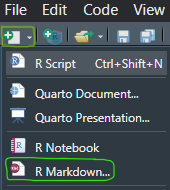
\includegraphics[width=\textwidth,height=1.04167in]{./img/rmd-click.png} or File \textgreater{} New File \textgreater{} R Markdown
\item
  \textbf{YAML header} defines format of the document as well as key info such as title, date, etc.
\item
  Text formatting:

  \begin{itemize}
  \tightlist
  \item
    \emph{italics} with \_italics\_
  \item
    \textbf{bold} with **bold**
  \item
    Unordered lists are created with -
  \item
    Ordered lists with 1., 2. \ldots{}
  \end{itemize}
\end{itemize}

\subsection{Last session}\label{last-session}

\begin{itemize}
\tightlist
\item
  Code chunks are inserted via the menu Code \textgreater{} Insert Chunk and should look like this:
\item
  ```\{r\}
  \# \emph{code goes here}
  ```

  \begin{itemize}
  \tightlist
  \item
    keyboard shortcut ctrl + alt + i / command + option + i
  \item
    Chunk options can specify how to treat code, e.g.~\texttt{echo\ =\ FALSE} only shows output but does not ``echo'' the actual code
  \end{itemize}
\item
  Indentation and spacing is very important! In the text, it is better to add more. In the YAML header, it may not be recognized properly with improper spacing
\end{itemize}

\subsection{Including Links \& Images}\label{including-links-images}

\begin{itemize}
\item
  An image to R Markdown is essentially a \textbf{link to an image file on your computer}

  \begin{itemize}
  \tightlist
  \item
    That's why they share similar notation
  \end{itemize}
\item
  \begin{longtable}[]{@{}l@{}}
  \toprule\noalign{}
  Web Link:** \\
  \midrule\noalign{}
  \endhead
  \bottomrule\noalign{}
  \endlastfoot
  ``\href{www.google.com}{Google Link}'' \\
  \end{longtable}

  \begin{itemize}
  \tightlist
  \item
    Becomes: \href{https://www.google.com/}{Google Link} (clickable Link)
  \end{itemize}
\item
  \textbf{Image:}
\end{itemize}

\begin{Shaded}
\begin{Highlighting}[]
\SpecialCharTok{!}\NormalTok{[image description](C}\SpecialCharTok{:}\ErrorTok{/}\NormalTok{path}\SpecialCharTok{/}\NormalTok{to}\SpecialCharTok{/}\NormalTok{your}\SpecialCharTok{/}\NormalTok{image.png)}
\end{Highlighting}
\end{Shaded}

\begin{itemize}
\item
  Different file formats, such as JPG, PNG, SVG or GIF
\item
  When including an image, make sure you are using the right file path, image name \& file extension! So that\ldots{}
\item
  ``
\includegraphics{"./img/rmd.png"}''
\item
  \ldots becomes\ldots{}
\item
  \begin{figure}
  \centering
  \includegraphics{./img/rmd.png}
  \caption{RMarkdown Logo}
  \end{figure}
\end{itemize}

\subsection{Inline Code}\label{inline-code}

\begin{itemize}
\tightlist
\item
  To simply include variables or values in text, we can use inline code `\emph{r code} `
\item
  Simply type one back tick ` and r - the program will auto complete the command
\item
  Examples:

  \begin{itemize}
  \tightlist
  \item
    The average sepal length of iris flowers is
    `\emph{r mean(iris\$Sepal.Length)}` \(\rightarrow\) 5.843
  \end{itemize}
\end{itemize}

\section{Taking full advantage of R}\label{taking-full-advantage-of-r}

\begin{enumerate}
\def\labelenumi{\arabic{enumi}.}
\tightlist
\item
  Conduct Analysis, e.g.~an ANOVA
\item
  Write about your analysis \& report results (with proper statistics)
\item
  Choose and create an appropriate visualization, e.g.~a boxplot
\end{enumerate}

\subsection{Walkthrough}\label{walkthrough}

We will use the package \texttt{palmerpenguins} (\texttt{install.packages("palmerpenguins")}) and see whether penguins from different islands have different body mass.

\begin{Shaded}
\begin{Highlighting}[]
\FunctionTok{library}\NormalTok{(palmerpenguins)}

\CommentTok{\# Test assumption of homoscedasticity}
\NormalTok{car}\SpecialCharTok{::}\FunctionTok{leveneTest}\NormalTok{(}\FunctionTok{aov}\NormalTok{(bill\_length\_mm }\SpecialCharTok{\textasciitilde{}}\NormalTok{ species, }\AttributeTok{data =}\NormalTok{ penguins)) }\CommentTok{\# yay}
\CommentTok{\# Levene\textquotesingle{}s Test for Homogeneity of Variance (center = median)}
\CommentTok{\#        Df F value Pr(\textgreater{}F)}
\CommentTok{\# group   2  2.2425 0.1078}
\CommentTok{\#       339}
\end{Highlighting}
\end{Shaded}

\begin{Shaded}
\begin{Highlighting}[]
\CommentTok{\# Run \& save ANOVA}
\NormalTok{penguinmodel }\OtherTok{\textless{}{-}} \FunctionTok{aov}\NormalTok{(bill\_length\_mm }\SpecialCharTok{\textasciitilde{}}\NormalTok{ species, }\AttributeTok{data =}\NormalTok{ penguins)}
\end{Highlighting}
\end{Shaded}

\subsection{Walkthrough}\label{walkthrough-1}

\begin{Shaded}
\begin{Highlighting}[]
\CommentTok{\# Run \& save post{-}hoc Tests}
\FunctionTok{TukeyHSD}\NormalTok{(penguinmodel)}
\CommentTok{\#   Tukey multiple comparisons of means}
\CommentTok{\#     95\% family{-}wise confidence level}
\CommentTok{\# }
\CommentTok{\# Fit: aov(formula = bill\_length\_mm \textasciitilde{} species, data = penguins)}
\CommentTok{\# }
\CommentTok{\# $species}
\CommentTok{\#                       diff       lwr        upr     p adj}
\CommentTok{\# Chinstrap{-}Adelie 10.042433  9.024859 11.0600064 0.0000000}
\CommentTok{\# Gentoo{-}Adelie     8.713487  7.867194  9.5597807 0.0000000}
\CommentTok{\# Gentoo{-}Chinstrap {-}1.328945 {-}2.381868 {-}0.2760231 0.0088993}
\end{Highlighting}
\end{Shaded}

\begin{itemize}
\item
  For anova, we want to report the full statistics, a.k.a ``full\_result'' from \texttt{papaja::apa\_print()}
\item
\begin{Shaded}
\begin{Highlighting}[]
\FunctionTok{library}\NormalTok{(papaja)}
\NormalTok{apa\_result }\OtherTok{\textless{}{-}} \FunctionTok{apa\_print}\NormalTok{(penguinmodel)}\SpecialCharTok{$}\NormalTok{full\_result}
\end{Highlighting}
\end{Shaded}
\end{itemize}

\subsection{Walkthrough}\label{walkthrough-2}

Create a boxplot and add results right in the caption!

\begin{Shaded}
\begin{Highlighting}[]
\FunctionTok{library}\NormalTok{(ggplot2)}
\FunctionTok{ggplot}\NormalTok{(penguins, }\FunctionTok{aes}\NormalTok{(}\AttributeTok{x=}\NormalTok{species, }\AttributeTok{y=}\NormalTok{bill\_length\_mm, }\AttributeTok{color=}\NormalTok{species, }\AttributeTok{fill=}\NormalTok{species), }\AttributeTok{na.rm=}\NormalTok{T) }\SpecialCharTok{+}
  \FunctionTok{geom\_boxplot}\NormalTok{(}\AttributeTok{alpha =}\NormalTok{ .}\DecValTok{7}\NormalTok{) }\SpecialCharTok{+} \FunctionTok{theme\_apa}\NormalTok{() }\SpecialCharTok{+} \FunctionTok{theme}\NormalTok{(}\AttributeTok{legend.position =} \StringTok{"none"}\NormalTok{) }\SpecialCharTok{+}
  \FunctionTok{labs}\NormalTok{(}\AttributeTok{x =} \StringTok{"Penguin Species"}\NormalTok{, }\AttributeTok{y =} \StringTok{"Bill Length (mm)"}\NormalTok{, }
       \AttributeTok{caption =}\NormalTok{ latex2exp}\SpecialCharTok{::}\FunctionTok{TeX}\NormalTok{(}\FunctionTok{unlist}\NormalTok{(apa\_result))) }\SpecialCharTok{+}
  \FunctionTok{scale\_color\_brewer}\NormalTok{(}\AttributeTok{palette =} \DecValTok{5}\NormalTok{) }\SpecialCharTok{+}
  \FunctionTok{scale\_fill\_brewer}\NormalTok{(}\AttributeTok{palette =} \DecValTok{5}\NormalTok{)}
\end{Highlighting}
\end{Shaded}

\includegraphics{_main_files/figure-html/unnamed-chunk-85-1.pdf}

\subsection{Walkthrough}\label{walkthrough-3}

\begin{itemize}
\tightlist
\item
  Note that it is a little complex to include the result right in the caption

  \begin{itemize}
  \tightlist
  \item
    ggplot2 cannot handle \LaTeX notation so we need to use package latex2exp
  \item
    the TeX function from that package cannot handle the list-output from apa\_print()\$full\_result so we need to ``unlist'' that
  \end{itemize}
\item
  Using RMarkdown, it is much easier to include the statistic right in the text with inline code:

  \begin{itemize}
  \tightlist
  \item
    `\emph{r apa\_print(penguinmodel)\$full\_result}`
  \item
    \(\rightarrow\) { \(F(2, 339) = 410.60\), \(p < .001\), \(\hat{\eta}^2_G = .708\), 90\% CI \([.669, .740]\) }
  \end{itemize}
\end{itemize}

\section*{Exercise}\label{exercise-8}
\addcontentsline{toc}{section}{Exercise}

Create an R Markdown Document that includes the same type of analyses of variance with all steps that we have conducted before.
Please use the \texttt{penguins} dataset from the \texttt{palmerpenguins} package and take ``species'' as the independent variable and ``flipper\_length\_mm'' as the dependent variable.

Solution

\begin{Shaded}
\begin{Highlighting}[]
\FunctionTok{leveneTest}\NormalTok{(}\FunctionTok{aov}\NormalTok{(flipper\_length\_mm }\SpecialCharTok{\textasciitilde{}}\NormalTok{ species, }\AttributeTok{data =}\NormalTok{ penguins))}
\NormalTok{penguinmodel2 }\OtherTok{\textless{}{-}} \FunctionTok{aov}\NormalTok{(bill\_length\_mm }\SpecialCharTok{\textasciitilde{}}\NormalTok{ species, }\AttributeTok{data =}\NormalTok{ penguins)}
\NormalTok{posthoc }\OtherTok{\textless{}{-}} \FunctionTok{TukeyHSD}\NormalTok{(penguinmodel2)}
\NormalTok{apa\_result }\OtherTok{\textless{}{-}} \FunctionTok{apa\_print}\NormalTok{(penguinmodel2)}\SpecialCharTok{$}\NormalTok{full\_result}

\FunctionTok{ggplot}\NormalTok{(penguins) }\SpecialCharTok{+}
  \FunctionTok{geom\_boxplot}\NormalTok{(}\FunctionTok{aes}\NormalTok{(}\AttributeTok{x =}\NormalTok{ species, }\AttributeTok{y =}\NormalTok{ flipper\_length\_mm, }\AttributeTok{color =}\NormalTok{ species, }\AttributeTok{fill =}\NormalTok{ species), }
               \AttributeTok{alpha =}\NormalTok{ .}\DecValTok{7}\NormalTok{, }\AttributeTok{na.rm =} \ConstantTok{TRUE}\NormalTok{) }\SpecialCharTok{+}
  \FunctionTok{theme\_apa}\NormalTok{() }\SpecialCharTok{+} 
  \FunctionTok{theme}\NormalTok{(}\AttributeTok{legend.position =} \StringTok{"none"}\NormalTok{) }\SpecialCharTok{+}
  \FunctionTok{labs}\NormalTok{(}\AttributeTok{x =} \StringTok{"Penguin Species"}\NormalTok{, }\AttributeTok{y =} \StringTok{"Flipper Length (mm)"}\NormalTok{) }\SpecialCharTok{+}
  \FunctionTok{scale\_color\_brewer}\NormalTok{(}\AttributeTok{palette =} \DecValTok{5}\NormalTok{) }\SpecialCharTok{+}
  \FunctionTok{scale\_fill\_brewer}\NormalTok{(}\AttributeTok{palette =} \DecValTok{5}\NormalTok{)}
\end{Highlighting}
\end{Shaded}

\section*{Wrap-Up \& Further Resources}\label{wrap-up-further-resources-9}
\addcontentsline{toc}{section}{Wrap-Up \& Further Resources}

Rmd offers many options for customization

Analyses can be conducted and reported in the same document

We can profit from many automatizations, e.g.~chapter numbering

Single values/ results can be reported with inline code

\href{https://www.markdownguide.org/basic-syntax/}{MarkdownGuide}

\href{https://www.markdownguide.org/cheat-sheet/}{Another Markdown Cheatsheet}

\href{https://statisticsglobe.com/ggsignif-package-r}{ggsignif package example}

\href{https://bookdown.org/yihui/rmarkdown-cookbook/bibliography.html}{Bibliography and Citation}

\begin{figure}
\centering
\includegraphics[width=\textwidth,height=4.6875in]{./img/palmer_penguins.png}
\caption{Palmer Penguins}
\end{figure}

\chapter*{Wrap Up}\label{wrap-up}
\addcontentsline{toc}{chapter}{Wrap Up}

If you have made it this far in the book, you should now posses the tools necessary to tackle most R tasks and more importantly, you should be able to teach yourself new skills.

In these last two Chapters I will share some last pieces of wisdom that may inspire you to keep learning R.
you will also find a collection of exercises and quiz questions to review your knowledge and hopefully have fun remembering it!
Personally, I got started because I had super talented people to learn from that I am glad to call my friends still today (Tobi, Lukas, Kilian - looking at you guys ).

If you found this book helpful and want to thank me or you have some suggestions or wishes for the future, please write me an email!
I hope to keep improving this intro and possibly adding to it, so I would also love to get some contributions!

So, here are my last pieces of wisdom inspired by things I learned and people I met at the \href{https://events.linuxfoundation.org/user/}{useR! conference 2024}:

\section*{Many people are working on many great projects.}\label{many-people-are-working-on-many-great-projects.}
\addcontentsline{toc}{section}{Many people are working on many great projects.}

\begin{Shaded}
\begin{Highlighting}[]
\NormalTok{ohwhaley}\SpecialCharTok{::}\FunctionTok{say}\NormalTok{(}\StringTok{"Thanks to Fonti Kar for this sweet whale package!"}\NormalTok{)}
\end{Highlighting}
\end{Shaded}

\section*{R can be hard.}\label{r-can-be-hard.}
\addcontentsline{toc}{section}{R can be hard.}

Which is why it's important to know a couple of tools to make your life easier.
Generally, I am hesitant to recommend using AI such as ChatGPT to help with coding, as it can be even more frustrating when this artificial companion suggests code that cannot work, cannot solve your problem, or simply confuses you even more.
Therefore, I suggest you have a look at \url{cs50.ai}, an AI developed to help with coding troubles by the Harvard university.

\begin{figure}
\centering
\includegraphics[width=\textwidth,height=3.125in]{./img/cs50ai.png}
\caption{CS50.ai example chat}
\end{figure}

\section*{\ldots{} but it's worth it.}\label{but-its-worth-it.}
\addcontentsline{toc}{section}{\ldots{} but it's worth it.}

R has a steep learning curve at the beginning, which can be frustrating but also means that it will keep getting easier to expand your skills.
For everyday use, i.e.~calculating statistics and creating visualizations, R is already great.
But it is possible to go much further: R has integrations for word processors (you've heard of LaTeX in R Markdown), building websites and apps (\href{https://shiny.posit.co/r/getstarted/shiny-basics/lesson1/index.html}{Shiny}), creating presentations (\href{https://quarto.org/docs/get-started/hello/rstudio.html}{Quarto}) and of course anyone can contribute to the community with new packages.
Try to stay curious and see if any of these features might be of use to you at some point!
Maybe you need to report a lot of your code and show visualizations in your thesis - why not write it in R Markdown?

\section*{R is really fun!}\label{r-is-really-fun}
\addcontentsline{toc}{section}{R is really fun!}

There are many reasons why so many people in so many fields of expertise choose this weird language\footnote{I highly recommend this lovely talk on \href{https://youtu.be/KOQBfC1WPwM?si=M_eStpWXBf56UGy7}{keeping R weird} by Kelly Bodwin.} as their primary means of communication.
One of them is definitely the powerful yet sometimes completely silly and useless things you can do with it (Thanks to Scott Chamberlain and Amanda Dobbyn for the package!):

\begin{Shaded}
\begin{Highlighting}[]
\NormalTok{cowsay}\SpecialCharTok{::}\FunctionTok{say}\NormalTok{(}\StringTok{"What the duck is this?"}\NormalTok{, }\AttributeTok{by =} \StringTok{"duck"}\NormalTok{)}
\end{Highlighting}
\end{Shaded}

\section*{Outlook}\label{outlook}
\addcontentsline{toc}{section}{Outlook}

Keep teaching yourself R - you have a lot of great resources!
And keep an open mind to keep finding cool features, such as the \texttt{emphatic} package, which lets you color rows in tables very easily.

\begin{Shaded}
\begin{Highlighting}[]
\NormalTok{iris }\SpecialCharTok{|\textgreater{}} 
  \FunctionTok{group\_by}\NormalTok{(Species) }\SpecialCharTok{|\textgreater{}} 
  \FunctionTok{summarize}\NormalTok{(}\AttributeTok{Mean\_Sepal\_Length =} \FunctionTok{mean}\NormalTok{(Sepal.Length)) }\SpecialCharTok{|\textgreater{}} 
\NormalTok{  emphatic}\SpecialCharTok{::}\FunctionTok{hl}\NormalTok{(}\FunctionTok{c}\NormalTok{(}\StringTok{"purple"}\NormalTok{, }\StringTok{"violet"}\NormalTok{, }\StringTok{"hotpink"}\NormalTok{))}
\end{Highlighting}
\end{Shaded}

Wrap-Up

R helps you to get an overview of your data

R gives your tools for data analysis \& visualization

R lets you create reports, presentations, app dashboards\ldots{}

Keep R weird! Do silly things in R!

Use the slides from this course as templates to learn from.

Further Resources

\href{https://solo-fsw.shinyapps.io/NewStatLearning/}{StatLearning Shiny App (Uni Leiden)}

\href{https://github.com/fontikar/ohwhaley}{GitHub: Ohwhaley package}

\href{https://www.youtube.com/@useRConference_global}{YouTube: useR! conference}

\chapter*{Practice}\label{practice}
\addcontentsline{toc}{chapter}{Practice}

\section{Loops: Write a for-loop that outputs the first X numbers of the Fibonacci sequence (``golden ratio'')}\label{loops-write-a-for-loop-that-outputs-the-first-x-numbers-of-the-fibonacci-sequence-golden-ratio}

\begin{figure}
\centering
\includegraphics[width=\textwidth,height=2.08333in]{./img/fibonacci.jpg}
\caption{Fibonacci Spiral}
\end{figure}

The Fibonacci sequence is defined as a sequence in which each number is the sum of the two proceeding ones.
That means, starting at 1 the sequence is: 1, 1, 2, 3, 5, 8, 13\ldots{}
Please create it for the first 15 numbers in the Fibonacci sequence and save the numbers to a variable called \emph{fibonacci}.

More info: \url{https://en.wikipedia.org/wiki/Fibonacci_sequence}.

Solution

\begin{Shaded}
\begin{Highlighting}[]
\NormalTok{n }\OtherTok{\textless{}{-}} \DecValTok{15}

\CommentTok{\# Simple and clear}
\NormalTok{fibonacci }\OtherTok{\textless{}{-}} \FunctionTok{c}\NormalTok{(}\DecValTok{1}\NormalTok{, }\DecValTok{1}\NormalTok{, }\FunctionTok{rep}\NormalTok{(}\ConstantTok{NA}\NormalTok{, n}\DecValTok{{-}2}\NormalTok{))}

\ControlFlowTok{for}\NormalTok{(i }\ControlFlowTok{in} \DecValTok{3}\SpecialCharTok{:}\NormalTok{n)\{}
\NormalTok{  fibonacci[i] }\OtherTok{\textless{}{-}}\NormalTok{ fibonacci[i}\DecValTok{{-}1}\NormalTok{] }\SpecialCharTok{+}\NormalTok{ fibonacci[i}\DecValTok{{-}2}\NormalTok{]}
\NormalTok{\}}
\NormalTok{fibonacci}
\CommentTok{\#  [1]   1   1   2   3   5   8  13  21  34  55  89 144 233 377 610}

\CommentTok{\# Alternative with while loop}
\NormalTok{fibonacci }\OtherTok{=} \FunctionTok{c}\NormalTok{(}\DecValTok{1}\NormalTok{, }\DecValTok{1}\NormalTok{)}

\ControlFlowTok{while}\NormalTok{(}\FunctionTok{length}\NormalTok{(fibonacci) }\SpecialCharTok{\textless{}}\NormalTok{ n)\{}
\NormalTok{  new\_num }\OtherTok{\textless{}{-}}\NormalTok{ fibonacci[}\FunctionTok{length}\NormalTok{(fibonacci)] }\SpecialCharTok{+}\NormalTok{ fibonacci[}\FunctionTok{length}\NormalTok{(fibonacci) }\SpecialCharTok{{-}} \DecValTok{1}\NormalTok{]}
\NormalTok{  fibonacci }\OtherTok{\textless{}{-}} \FunctionTok{c}\NormalTok{(fibonacci, new\_num)}
\NormalTok{\}}
\NormalTok{fibonacci}
\CommentTok{\#  [1]   1   1   2   3   5   8  13  21  34  55  89 144 233 377 610}
\end{Highlighting}
\end{Shaded}

\section{RMarkdown: Start your document in a certain way that matches the template!}\label{rmarkdown-start-your-document-in-a-certain-way-that-matches-the-template}

Look at the example document shown below and try to re-create it!
Be mindful of which elements need to be defined in the YAML header and which need to be modified in the text.

\begin{figure}
\centering
\includegraphics[width=\textwidth,height=5.72917in]{./img/Rmd-exc1.png}
\caption{Rmd Example Template}
\end{figure}

Solution

\begin{Shaded}
\begin{Highlighting}[]
\SpecialCharTok{{-}{-}{-}}
\NormalTok{title}\SpecialCharTok{:} \StringTok{"Exercise 1"}
\NormalTok{author}\SpecialCharTok{:} \StringTok{"A great author"}
\NormalTok{date}\SpecialCharTok{:} \StringTok{"2024{-}07{-}02"}
\NormalTok{output}\SpecialCharTok{:} 
\NormalTok{  pdf\_document}\SpecialCharTok{:}
\NormalTok{    toc}\SpecialCharTok{:}\NormalTok{ true}
\SpecialCharTok{{-}{-}{-}}

\CommentTok{\# First Chapter}

\NormalTok{Some text }\ControlFlowTok{in} \SpecialCharTok{**}\NormalTok{bold}\SpecialCharTok{**}\NormalTok{.}

\DocumentationTok{\#\# A subchapter}

\NormalTok{Some text }\ControlFlowTok{in}\NormalTok{ \_cursive\_.}

\CommentTok{\# Second Chapter}

\NormalTok{Here is an overview of the iris dataset}\SpecialCharTok{:}

\StringTok{\textasciigrave{}\textasciigrave{}}\NormalTok{\{r\} }\CommentTok{\# make sure to include three \textasciigrave{} here!}
\FunctionTok{head}\NormalTok{(iris, }\DecValTok{3}\NormalTok{)}
\StringTok{\textasciigrave{}\textasciigrave{}}
\end{Highlighting}
\end{Shaded}

Hadley Wickham GIFfrom Hadley GIFs

\chapter*{Toolbox}\label{toolbox}
\addcontentsline{toc}{chapter}{Toolbox}

The toolbox contains a collection of nifty tips, tricks and hacks for anything R.

\section*{Keyboard shortcuts to make your life easier}\label{shortcuts}
\addcontentsline{toc}{section}{Keyboard shortcuts to make your life easier}

\begin{longtable}[]{@{}ll@{}}
\toprule\noalign{}
Function & Shortcut PC / Mac \\
\midrule\noalign{}
\endhead
\bottomrule\noalign{}
\endlastfoot
Run current line & Ctrl + Enter / Cmd + Return \\
Add \textless- & Alt + - / Option + - \\
Add \%\textgreater\% & Ctrl + Shift + M / Cmd + Shift + M \\
Show help & F1 \\
Options for auto-fill & Tab \\
Create New Script & Ctrl + Shift + N / Cmd + Shift + N \\
Comment out line & Ctrl + Shift + C / Cmd + Shift + C \\
Save your script & Ctrl + S / Cmd + S \\
\end{longtable}

\section*{Reading in Data}\label{reading-in-data}
\addcontentsline{toc}{section}{Reading in Data}

\begin{longtable}[]{@{}ll@{}}
\toprule\noalign{}
Data Source & R command \\
\midrule\noalign{}
\endhead
\bottomrule\noalign{}
\endlastfoot
WEXTOR (CSV) & \texttt{readr::read\_delim("data.csv",\ delim\ =\ ";")} \\
Excel (XLSX) & \texttt{xlsx::read.xlsx("data.xlsx",\ sheetIndex\ =\ 1)} \\
R Data Source (RDS) & \texttt{readRDS("data.Rds")} \\
SPSS (SAV) & \texttt{foreign::read.spss("data.sav")} \\
\end{longtable}

\section*{Logic}\label{logic-1}
\addcontentsline{toc}{section}{Logic}

\begin{longtable}[]{@{}
  >{\raggedright\arraybackslash}p{(\columnwidth - 2\tabcolsep) * \real{0.4667}}
  >{\raggedright\arraybackslash}p{(\columnwidth - 2\tabcolsep) * \real{0.5333}}@{}}
\toprule\noalign{}
\begin{minipage}[b]{\linewidth}\raggedright
Symbol
\end{minipage} & \begin{minipage}[b]{\linewidth}\raggedright
Meaning
\end{minipage} \\
\midrule\noalign{}
\endhead
\bottomrule\noalign{}
\endlastfoot
\textless{} & smaller than \\
\textless= & smaller or equal \\
\textgreater{} & greater than \\
\textgreater= & greater or equal \\
== & equal to \\
!= & unequal to \\
TRUE & true (also written T) \\
FALSE & false (also written F) \\
\texttt{tidyselect::between(x,\ left,\ right)} & is x between the left and right value? \\
\texttt{tidyselect::contains(match)} & selects columns whose names contain a word (to be used with \texttt{dplyr::select()}) \\
\& & AND (both must be TRUE) \\
\textbar{} & OR (just one must be TRUE) \\
! & NOT (as in != NOT equal) \\
\end{longtable}

\section*{\texorpdfstring{Most important \texttt{dplyr} functions}{Most important dplyr functions}}\label{mif}
\addcontentsline{toc}{section}{Most important \texttt{dplyr} functions}

\begin{itemize}
\tightlist
\item
  \texttt{select()}: select certain columns by name
\item
  \texttt{filter()}: filter values from a column/variable
\item
  \texttt{rename()}: rename a variable
\item
  \texttt{mutate()}: change values of a column (new or existing)
\item
  \texttt{\%\textgreater{}\%}: ``pipe'' brings data from previous operation to the next (Shortcut: Strg + Shift + M)
\end{itemize}

\section*{Incomplete List of Useful Packages}\label{lop}
\addcontentsline{toc}{section}{Incomplete List of Useful Packages}

\begin{longtable}[]{@{}ll@{}}
\toprule\noalign{}
Package Name & General Purpose \\
\midrule\noalign{}
\endhead
\bottomrule\noalign{}
\endlastfoot
psych & Advanced statistical testing / modeling e.g.~factor analysis \\
tibble & Alternative for creating data frames \\
tidyr & Clean up daata \& simple reshaping \\
dropR & Dropout analysis (by experimental condition) \\
foreign & Handling data from SPSS \\
corrplot & Create correlation plots/ matrices \\
\end{longtable}

  \bibliography{book.bib,packages.bib}

\end{document}
